\documentclass{rgn}
\usetikzlibrary{arrows,decorations.markings}
\usetikzlibrary{shapes, arrows, positioning}
\usetikzlibrary{patterns}
\usetikzlibrary{decorations.pathmorphing,patterns}
\usetikzlibrary{math}
\usepackage{xpatch}
\pgfplotsset{width=15cm, compat=1.15}

\usetikzlibrary{external}
\tikzexternalize[prefix=figures/]
%\tikzset{external/system call={pdflatex \tikzexternalcheckshellescape -halt-on-error -interaction=batchmode}}

%strelice
\tikzset{strelica1/.style={decoration={markings,mark=at position 1 with %
    {\arrow[scale=2,>=latex']{>}}},postaction={decorate}}}

\tikzset{strelica0/.style={decoration={markings,mark=at position 0 with %
    {\arrow[scale=2,>=latex']{<}}},postaction={decorate}}}

%naredbe
\newcommand{\ltr}{\mathcal{L}}	%operator laplaceove transformacije
\newcommand\ffrac[2]{\frac{\displaystyle #1}{\displaystyle #2}}
\newcommand\vtor[2]{
    \IfEqCase{#2}{%
        {}{\{#1\}}%
        {.}{\{\dot{#1}\}}%
        {:}{\{\ddot{#1}\}}%
    }%
}
\newcommand\mm{\mathbf{m}}
\newcommand\kk{\mathbf{k}}
\newcommand\cc{\mathbf{c}}
\newcommand\ppsi{\mathbf{\Psi}}
\newcommand\oomega{\mathbf{\Omega}}
\newcommand\K{\mathbf{K}}
\newcommand\M{\mathbf{M}}
\newcommand\C{\mathbf{C}}

%argumenti #1 - x_0 #2 - y_0 \dx - x_1 #4 - y_1
\newcommand{\prigusivac}[4]{%
    \tikzmath{\dx = #3 - #1;}
    \tikzmath{\dy = #4 - #2;}
    \draw[thick](#1, #2) -- ({\dx/2-0.5}, {\dy/2+#2});
    \draw[thick]({\dx/2-0.5}, {(\dy/2+#2}) -- ({\dx/2-0.1}, {\dy/2+#2});
    \draw[thick]({\dx/2+0.1}, {\dy/2+#2}) -- ({\dx/2+0.5}, {\dy/2+#2});
    \draw[thick]({\dx/2+0.5}, {\dy/2+#2}) -- (#3, #4);

    \draw[thick]({\dx/2-0.1}, {\dy/2+#2-0.3}) -- ({\dx/2-0.1}, {\dy/2+#2+0.3});
    \draw[thick]({\dx/2-0.1}, {\dy/2+#2-0.3}) -- ({\dx/2+0.25}, {\dy/2+#2-0.3});
    \draw[thick]({\dx/2-0.1}, {\dy/2+#2+0.3}) -- ({\dx/2+0.25}, {\dy/2+#2+0.3});

    \draw[thick]({\dx/2+0.1}, {\dy/2+#2+0.2}) -- ({\dx/2+0.1}, {\dy/2+#2-0.2});
}
\author{Ivan Bakula} 
\rad{Diplomski rad}
\studij{Diplomski studij rudarstva}
\indeks{R-262}
\title{Odziv dinamičkog sistema na harmonijsku pobudu}
\godina{2021}

\begin{document}

\maketitle
%\includepdf[pages={1}]{../rjesenje.pdf}
%titlepage zato da ne numerira karticu (prljav trik)
\begin{titlepage}
    \input{kartica_hr}
\end{titlepage}
\begin{titlepage}
    {\large \fontsize{10}{13}\selectfont{%
% @{} - znaci: poravnaj prvi stupac s okolnim tekstom (ne uvlaci za 6pt)
\begin{tabularx}{\textwidth} {@{} X r}
    University of Zagreb & Master's Thesis\\
    Faculty of Mining, Geology and Petroleum Engineering & 
\end{tabularx}

\vskip 6mm

\begin{center}
    DYNAMIC SYSTEM RESPONSE TO HARMONIC EXCITATION\\[6pt]
    IVAN BAKULA
\end{center}

\begin{tabular}{@{}l l}
    Thesis completed at:      & University of Zagreb\\
                              & Faculty of Mining, Geology and Petroleum Engineering\\
                              & Department of Mining Engineering and Geotechnics\\
                              & Pierottijeva 6, 10 000 Zagreb
\end{tabular}
\par

Abstract:
\par
This paper examines system response to harmonic excitation, first discussing the
single degree of freedom (sdof) system response, followed by analyzing the multiple
degree of freedom (mdof) system response. It discusses response characteristics,
frequency response functions, as well as the concept of resonance, and analyzes the
theory's experimental application. The mdof system analysis starts with a discussion
on the steady state response, for which modal analysis is not necessary, and
continues with the application of the modal analysis.
\vskip 5mm

Keywords: harmonic excitation, single degree of freedom system, multiple degree of
freedom system, frequency response function, resonancce, modal analysis 
\vskip 5mm

Diplomski rad sadrži: \totalpages{} pages, \totaltables{} table, \totalfigures{} figures, 6 references.

\vskip 5mm

Original in: Croatian 

\vskip 5mm

\begin{tabular}{@{}l l}
    Archived in:             & Library of Faculty of Mining, Geology and Petroleum Engineering\\
                             & Pierottijeva 6, Zagreb
\end{tabular}
\par

\vskip 6mm
Supervisor: Associate professor Antonia Jaguljnjak Lazarević, PhD 
\vskip 5mm

\begin{tabular}{@{}l l}
    Reviewers:   & 1. Associate professor Antonia Jaguljnjak Lazarević, PhD\\
                 & 2. Associate professor Petar Hrženjak, PhD\\
                 & 3. Tenured professor Željko Andreić, PhD
\end{tabular}

\vfill

Defence date: February 12, 2021, Faculty of Mining, Geology and Petroleum
Engineering, University of Zagreb
}}
\newpage

\end{titlepage}

\frontmatter
\tableofcontents
\newpage
\listoftables
\newpage
\listoffigures
\newpage
\chapter*{Popis korištenih oznaka i pripadajućih SI jedinica}
\begin{tabularx}{\textwidth}{X l l}
    Oznaka                      & Opis                                      & Jedinica\\
    $m$                         & masa                                      & $kg$\\
    $k$                         & krutost                                   & $Nm^{-1}$\\
    $c$                         & koeficijent viskoznog prigušenja          & $kgs^{-1}$\\
    $c_kr$                      & kritično prigušenje                       & $kgs^{-1}$\\
    $F_S$                       & unutarnja sila                            & $N$\\
    $F_D$                       & sila prigušenja                           & $N$\\
    $u$                         & pomak                                     & $m$\\
    $\dot{u},\, v$              & brzina                                    & $m{s^-1}$\\
    $\ddot{u}$                  & ubrzanje                                  & $ms^{-2}$\\
    $p_0$                       & amplituda                                 & $m$\\
    $\sigma$                    & stupanj prigušenja                        & $s^{-1}$\\
    $\omega_D$                  & vlastita frekvencija prigušenog titranja  & $s^{-1}$\\
    $\omega_n$                  & prirodna frekvencija                      & $s^{-1}$\\
    $i$                         & imaginarna jedinica                       & \\
    $R_d$                       & dinamički faktor pomaka                   & \\
    $R_v$                       & dinamički faktor brzine                   & \\
    $R_a$                       & dinamički faktor ubrzanja                 & \\
    $\vtor{\psi}{}_n$           & vlastiti vektori (oblici titranja)        & \\
    $\omega$                    & vlastite vrijednosti (prirodne frekvencije) & $s^{-1}$\\
    $\ppsi$                     & modalna matrica                           & \\
    $\oomega$                   & spektralna matrica                        & $[s^{-1}]$\\
    $\mm$                       & matrica masa                              & $[kg]$\\
    $\kk$                       & matrica krutosti                          & $[Nm^{-1}]$\\
    $M_{n,n}$                   & modalna masa                              & $kg$\\
    $K_{n,n}$                   & modalna krutost                           & $Nm^{-1}$\\
    $\M$                        & matrica modalnih masa                     & $[kg]$\\
    $\K$                        & matrica modalnih krutosti                 & $[Nm^{-1}]$\\
    $\C$                        & matrica modalnih prigušenja               & $[kgs^{-1}]$ 
\end{tabularx}

\mainmatter
\chapter{Uvod}
    Dinamičke pobude izuzetno su česta pojava u tehnologiji. Primjerice, u
graditeljstvu, strojarstvu i sl. dinamičkom pobudom smatramo djelovanje sile
čiji se intenzitet mijenja tijekom vremena. Takva sila može biti zadana funkcijom
$p(t) = p_0 \sin(\omega t)$. Dinamički sustav je svaki sustav pod utjecajem dinamičke pobude, a 
rezultat djelovanja pobude je odziv. 

\begin{figure}[H]
    \begin{subfigure}{0.3\textwidth}
        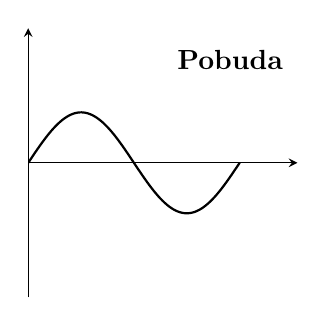
\begin{tikzpicture}
    \begin{axis} [
        title style={at={(0.75,0.75)},anchor=south,yshift=-0.1},
        title = \bfseries{Pobuda},
        ticks = none,
        width = 5cm, height = 5cm,
        xmin = 0, xmax = 8,
        ymin = -2, ymax = 2,
        axis x line = center,
        axis y line = center
    ]
        \addplot [
            domain  = 0:6.283185307179586,
            samples = 100,
            color   = black,
            thick,
        ]{0.75 * sin(deg(x))};
    \end{axis}

\end{tikzpicture}

    \end{subfigure}
    \hskip 1pt
    \begin{subfigure}{0.3\textwidth}
        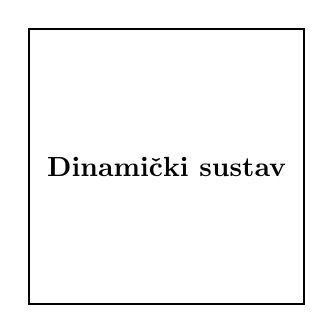
\begin{tikzpicture}
    %sustav
    \draw[thick] (0, 0) rectangle (3.5, 3.5); 
    \node at (1.75, 1.75) {\bfseries{Dinamički sustav}};
\end{tikzpicture}

    \end{subfigure}
    \hskip 1pt
    \begin{subfigure}{0.3\textwidth}
        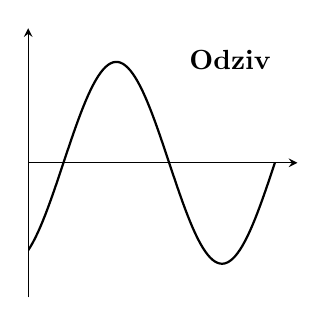
\begin{tikzpicture}
    \begin{axis} [
        title style={at={(0.75,0.75)},anchor=south,yshift=-0.1},
        title = \bfseries{Odziv},
        ticks = none,
        width = 5cm, height = 5cm,
        xmin = 0, xmax = 8,
        ymin = -2, ymax = 2,
        axis x line = center,
        axis y line = center
    ]
        \addplot [
            domain  = 0:7.330382858376184,
            samples = 100,
            color   = black,
            thick,
        ]{1.5* sin(deg(x) - deg(1.047197))};
    \end{axis}

\end{tikzpicture}

    \end{subfigure}
    \caption{Shematski prikaz dinamičkog sustava}
    \label{fig:shematski_prikaz_sustava}
\end{figure}

Sa shematskoga prikaza \ref{fig:shematski_prikaz_sustava} može se naslutiti da su pobuda 
i odziv u međusobnoj sprezi. Navedenom spregom "upravlja" dinamički sustav. U slučaju da 
dinamički sustav pripada razredu linearnih sustava, sprega između pobude i odziva zadana 
je konvolucijom pobude s prijenosnom funkcije sustava. Sama prijenosna funkcija određena 
je diferencijalnom jednadžbom sustava. 
\par

%Većina dinamičkih sustava iz tehnologije zaista spada u kategoriju linearnih sustava. 
%Da bi određeni dinamički sustav bio i linearni sustav mora zadovoljiti slijedeća 
%svojstva: 
%\begin{enumerate}
%    \item aditivnost
%    \item homogenost
%    \item fazni pomak u pobudi rezultira identičnim faznim pomakom u odzivu
%    \item statička linearnost - nije nužan uvjet, ali je poslijedica prethodna tri
%\end{enumerate}
%
%\par
%Objasni svojstva
%\par

U ovome se radu razmatra mehanički linearni sustav najprije s jednim, a
zatim i s više stupnjeva slobode pod utjecajem harmonijske sile $p(t) = p_0 \sin(\omega t)$. 
Teorijski koncepti izvedeni za linearni sustav s jednim stupnjem slobode koriste se  
u razvoju eksperimentalnih metoda za određivanje perioda stupnja prigušenja realnih 
konstrukcija. 
\par

Cilj ovog rada jest upoznavanje s osnovnim teorijskim i praktičnim znanjima iz
dinamike konstrukcija. 


\chapter{Sustavi s jednim stupnjem slobode}
    \section{Model sustava s jednim stupnjem slobode}
Modeli sustava s jednim stupnjem slobode su posmični okviri, a možemo ih shvatiti
kao idealizaciju jednokatnice. Posmični okviri se sastoje od štapova, koncentrirane
mase i viskoznog prigušivača, pri čemu je ukupna krutost sustava sadržana u krutosti
štapova, ukupna masa sustava u koncentriranoj masi i ukupno prigušenje u viskoznom
prigušivaču. Nadalje, vrijedi pretpostavaka o vertikalnoj i horizontalnoj
nestišljivosti štapova, tj. štapovi su nepromjenjive dužine.
\par
\begin{figure}[H]
    \begin{subfigure}[b]{0.5\textwidth}\label{fig:priguseni-sustav-sdf}
        \centering
        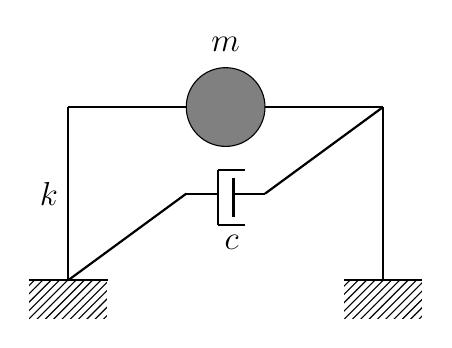
\begin{tikzpicture}
%štapovi
	\draw[thick] (0,0) -- (0,2.2)
		node[pos=0.5,left]{\textbf{\large{$k$}}};
	\draw[thick] (0,2.2) -- (4,2.2);
	\draw[thick] (4,0) -- (4,2.2);
	
%masa
	\filldraw[color=black, fill=gray] (2,2.2) circle (0.5);
	\node[draw=none, fill=none]  at(2, 3)
		{\textbf{\large{$m$}}};

%viskozni prigusivac
	\draw[thick] (0, 0) -- (1.5, 1.1);
	\draw[thick] (1.5, 1.1) -- (1.9, 1.1);
	\draw[thick] (2.1, 1.1) -- (2.5, 1.1);
	\draw[thick] (2.5, 1.1) -- (4, 2.2);

	\draw[thick] (1.9, 0.7) -- (1.9, 1.4);
	\draw[thick] (1.9, 1.4) -- (2.25, 1.4);
	\draw[thick] (1.9, 0.7) -- (2.25, 0.7)
		node[pos=0.5, below]{\textbf{\large{$c$}}};

	\draw[thick] (2.1, 1.3) -- (2.1, 0.8);


%podloga
	\draw[white, pattern=north east lines, pattern color=black] (-0.5, 0) rectangle (0.5, -0.5);
	\draw[thick] (-0.5, 0) -- (0.5, 0);

	\draw[white, pattern=north east lines, pattern color=black] (3.5, 0) rectangle (4.5, -0.5);
	\draw[thick] (3.5, 0) -- (4.5, 0);
\end{tikzpicture}

        \caption{Posmični okvir s prigušenjem}
    \end{subfigure}
    \hfill
    \begin{subfigure}[b]{0.5\textwidth}\label{fig:priguseni-ekvivalentni-sustav-sdf}
        \centering
        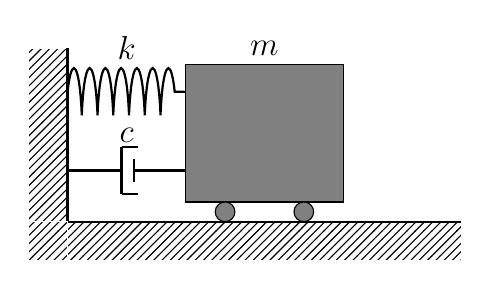
\begin{tikzpicture}
	%podloga
	\draw[white, pattern=north east lines, pattern color=black] (0, 0)
	rectangle (-0.5, 2.2);
	\draw[thick] (0,0) -- (0, 2.2);

	\draw[white, pattern=north east lines, pattern color=black] (0, 0) 
	rectangle (5, -0.5);
	\draw[thick] (0,0) -- (5,0);
	
	\draw[white, pattern=north east lines, pattern color=black] (0, 0)
	rectangle (-0.5, -0.5);

	%uteg
	\filldraw[fill=gray] (1.5, 2) rectangle (3.5, 0.25);

	%kotaci
	\filldraw[fill=gray] (2, 0.125) circle (0.125);
	\filldraw[fill=gray] (3, 0.125) circle (0.125);

	%opruga
	\draw[thick, decoration={aspect=0.1, segment length=2mm,amplitude=3mm,coil},decorate] (0,1.65) -- (1.5, 1.65);

	%prigusivac
	\draw[thick] (0, 0.65) -- (0.685, 0.65);
	\draw[thick] (0.84, 0.65) -- (1.5, 0.65);

	\draw[thick] (0.685, 0.35) -- (0.685, 0.95);
	\draw[thick] (0.685, 0.95) -- (0.9, 0.95);
	\draw[thick] (0.685, 0.35) -- (0.9, 0.35);

	\draw[thick] (0.84, 0.5) -- (0.84, 0.8);

        \node[draw=none, fill=none] at (0.75, 2.2) {\textbf{\large{$k$}}}; 
        \node[draw=none, fill=none] at (2.5,   2.2) {\textbf{\large{$m$}}};
        \node[draw=none, fill=none] at (0.75, 1.1) {\textbf{\large{$c$}}};

\end{tikzpicture}

        \caption{Ekvivalentni model s prigušenjem}
    \end{subfigure}
    \vfill
    \begin{subfigure}[b]{0.5\textwidth}\label{fig:nepriguseni-sustav-sdf}
        \centering
        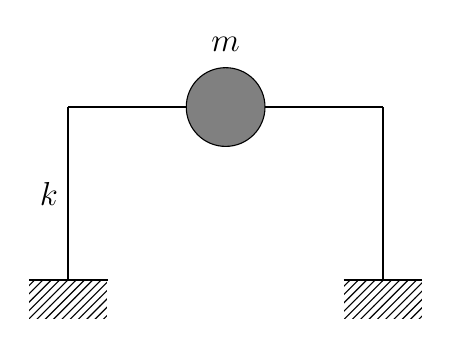
\begin{tikzpicture}
%štapovi
	\draw[thick] (0,0) -- (0,2.2)
		node[pos=0.5,left]{\textbf{\large{$k$}}};
	\draw[thick] (0,2.2) -- (4,2.2);
	\draw[thick] (4,0) -- (4,2.2);
	
%masa
	\filldraw[color=black, fill=gray] (2,2.2) circle (0.5);
	\node[draw=none, fill=none] at(2,3) 
	{\textbf{\large{$m$}}};

%podloga
	\draw[white, pattern=north east lines, pattern color=black] (-0.5, 0) 
	rectangle (0.5, -0.5);
	\draw[thick] (-0.5, 0) -- (0.5, 0);

	\draw[white, pattern=north east lines, pattern color=black] (3.5, 0)
	rectangle (4.5, -0.5);
	\draw[thick] (3.5, 0) -- (4.5, 0);
\end{tikzpicture}

        \caption{Posmični okvir bez prigušenja}
    \end{subfigure}
    \hfill
    \begin{subfigure}[b]{0.5\textwidth}\label{fig:nepriguseni-ekvivalentni-sustav-sdf}
        \centering
        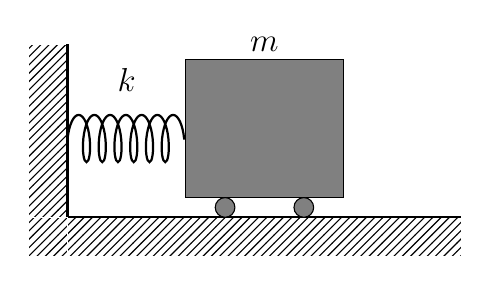
\begin{tikzpicture}
	%podloga
	\draw[white, pattern=north east lines, pattern color=black] (0, 0)
	rectangle (-0.5, 2.2);
	\draw[thick] (0,0) -- (0, 2.2);

	\draw[white, pattern=north east lines, pattern color=black] (0, 0) 
	rectangle (5, -0.5);
	\draw[thick] (0,0) -- (5,0);
	
	\draw[white, pattern=north east lines, pattern color=black] (0, 0)
	rectangle (-0.5, -0.5);

	%uteg
	\filldraw[fill=gray] (1.5, 2) rectangle (3.5, 0.25);

	%kotaci
	\filldraw[fill=gray] (2, 0.125) circle (0.125);
	\filldraw[fill=gray] (3, 0.125) circle (0.125);

	%opruga
	\draw[thick, decoration={aspect=0.3, segment length=2mm,amplitude=3mm,coil},decorate] (0,1) -- (1.5, 1);

	\node[draw=none, fill=none] at (0.75, 1.75) {\textbf{\large{$k$}}}; 
	\node[draw=none, fill=none] at (2.5,   2.2) {\textbf{\large{$m$}}};

\end{tikzpicture}

        \caption{Ekvivalentni model bez prigušenja}
    \end{subfigure}
    \caption{Idealizirani sustav s jednim stupnjem slobode}
\end{figure}

Primjetimo da navedeni sustav s pogleda statike predstavlja ravninski problem s tri
stupnja slobode (dvije rotacije u zglobovima te translacija), stoga ga je potrebno
svesti na sustav s jednim stupnjem slobode za potrebe dinamičkog proračuna. Drugim
riječima, potrebno je ukupnu krutost sustava izraziti kao lateralnu krutost.
Postupak svođenja sustava s tri stupnja slobode na sustav s jednim stupnjem slobode
naziva se \textit{statička kondenzacija} koju u ovom radu nećemo razmatrati.
\newpage


    \newpage
    \section{Jednadžba gibanja modela pri sinusnoj pobudi}
Dijagram sila za sustav s prigušenjem na koji djeluje sila pobude $p(t)$ prikazan je
na slijedećoj slici:

\begin{figure}[H]
    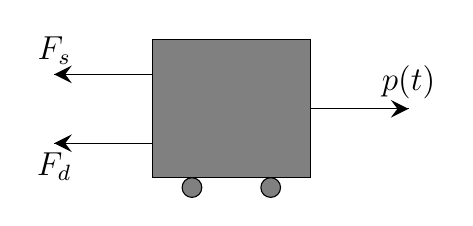
\begin{tikzpicture}
%povecaj strelice
\tikzset{myptr/.style={decoration={markings,mark=at position 1 with %
    {\arrow[scale=2,>=stealth]{>}}},postaction={decorate}}}

	%podloga
%	\draw[white, pattern=north east lines, pattern color=gray] (0, 0)
%	rectangle (-0.5, 2.2);
%	\draw[thick] (0,0) -- (0, 2.2);

%	\draw[white, pattern=north east lines, pattern color=gray] (0, 0) 
%	rectangle (5, -0.5);
%	\draw[thick] (0,0) -- (5,0);
	
%	\draw[white, pattern=north east lines, pattern color=gray] (0, 0)
%	rectangle (-0.5, -0.5);

	%uteg
	\filldraw[fill=gray] (1.5, 2) rectangle (3.5, 0.25);

	%kotaci
	\filldraw[fill=gray] (2, 0.125) circle (0.125);
	\filldraw[fill=gray] (3, 0.125) circle (0.125);

	%sile
	\draw[myptr] (1.5, 1.5625) -- (0.25, 1.5625) 
		node[pos=1, above]{\textbf{\large{$F_s$}}};
	\draw[myptr] (1.5, 0.6875) -- (0.25, 0.6875)
		node[pos=1, below]{\textbf{\large{$F_d$}}};
	\draw[myptr] (3.5, 1.125) -- ( 4.75, 1.125) 
		node[pos=1, above]{\textbf{\large{$p(t)$}}};

\end{tikzpicture}

    \label{fig:sile-priguseni-ekvivalentni-sustav-sdf}
    \caption{Dijagram sila ekvivalentnog modela prigušenog linearnog sustava s jednim stupnjem slobode}
\end{figure}

Prema drugom Newtonovom aksiomu vrijedi:
\begin{align}
    \Sigma F = ma = m\ddot{u}\notag\\
        p(t) - F_S - F_D = m\ddot{u} \notag\\
        m\ddot{u} + F_S + F_D = p(t) \label{eq:newton}
\end{align}

Gdje je:\\
\begin{table}[H]
\begin{tabular}{c l}
	$F_S$ & unutarnja sila \\
	$F_D$ & sila prigušenja \\
	$m$   & masa \\
        $a,\ddot{u}$   & ubrzanje\\
\end{tabular}
\end{table}

Unutarnju silu možemo zapisati kao:
\begin{equation}
	F_S = k \cdot u \label{eq:hooke}
\end{equation}

A silu prigušenja kao:
\begin{equation}
	F_D = c \cdot v = c \cdot \dot{u} \label{eq:prigusenje}
\end{equation}

Gdje je:\\
\begin{table}[H]
\begin{tabular}{c l}
	$k$ & krutost \\
	$c$ & koeficijent viskoznog prigušenja \\
	$u$ & pomak \\
	$\dot{u},v$ & brzina \\
\end{tabular}
\end{table}

Uvrštavanjem \eqref{eq:hooke} i \eqref{eq:prigusenje} u \eqref{eq:newton} dobijemo:
\begin{equation}
	m\ddot{u} + c\dot{u} + ku = p(t) \label{eq:jednadzba_opcenita_pobuda}
\end{equation}

Sila pobude $p(t)$ je sinusna sila $p_0sin(\omega t)$, pri čemu je $p_0$ amplituda, a
$\omega$ frekvencija, stoga jednadžba pod \eqref{eq:jednadzba_opcenita_pobuda}
postaje:
\begin{equation}
	m\ddot{u} + c\dot{u} + ku = p_0sin(\omega t)
\label{eq:jednadzba_sinusna_pobuda}
\end{equation} 


Jednadžba pod \eqref{eq:jednadzba_sinusna_pobuda} jest nehomogena linearna
diferencijalna jednadžba drugog reda, a riještiti ćemo ju primjenom Laplaceove
transformacije\footnote{Iako postupkom dugotrajnija (u ovom
slučaju), metoda Laplaceove transformacije nam pruža jedinstven uvid u međudjelovanje sustava
i pobude.}.
\par

Transformiranjem jednadžbe \eqref{eq:jednadzba_sinusna_pobuda} dobijemo 
slijedeću algebarsku jednadžbu u frekvencijskoj domeni:
\begin{equation}\label{eq:transformat_diferencijalna}
        m(s^2U(s)-su(0)-\dot{u}(0))+
	c(sU(s)-u(0))+
	kU(s) = 
        P(s)
\end{equation}
Gdje je $P(s)$ transformat funkcije $p(t)=p_0\sin(\omega t)$.
Sređivanjem \eqref{eq:transformat_diferencijalna} dobijemo: 
\begin{equation}\label{eq:transformat_diferencijalna_sredjeno}
    U(s)\left(ms^2+cs+k\right)-msu(0)-m\dot{u}-cu(0) = P(s)
\end{equation}

Jednadžbu \eqref{eq:transformat_diferencijalna_sredjeno} možemo rastaviti na više logičnih
cijelina:
\begin{alignat}{2}
    &\text{Dinamička krutost} & Z(s)&=ms^2+cs+k\label{eq:din_krutost}\\
    &\text{Prijenosna funkcija sustava}\quad & H(s)&=\frac{1}{Z(s)}=\frac{1}{ms^2+cs+k}\label{eq:prijenosna}\\
    &\text{Pobuda početnim uvjetima}\quad & W(s)&=(ms+c)u(0)+m\dot{u}\label{eq:pobuda_pocetni}\\
    &\text{Pobuda sinusnom silom} & P(s)&=p_0\frac{\omega}{s^2+\omega^2}\label{eq:pobuda_sinusna}
\end{alignat}

Uvrštavanjem \eqref{eq:prijenosna},\eqref{eq:pobuda_pocetnim_uvjetima} u 
\eqref{eq:transformat_diferencijalna_sredjeno} dobijemo:
\begin{equation*}
	\frac{U(s)}{H(s)}=W(s)+P(s)
\end{equation*}

Množenjem prijenosnom funkcijom sustava ($H(s)$) dobijemo:
\begin{equation}
	U(s)=\underbrace{H(s)W(s)}_{\substack{\text{konvolucija u}\\\text{vremenskoj
	domeni}}}
	+ 
	\underbrace{H(s)P(s)}_{\substack{\text{konvolucija u}\\\text{vremenskoj domeni}}}
\end{equation}

Pri čemu je:
\begin{table}[H]
\begin{tabular}{c l}
	$H(s)\cdot W(s)$ & odziv na pobudu početnim uvjetima u frekvencijskoj domeni\\
	$H(s)\cdot P(s)$ & odziv na pobudu sinusnom silom u frekvencijskoj domeni\\
\end{tabular}
\end{table}

\newpage
Da bi bilo lakše naći inverze odziva u frekvencijskoj domeni potrebno je funkciju  
$H(s)$ prikazati u tabličnom obliku\footnote{postupak svođenja prijenosne funkcije
sustava na tablični oblik prikazan je u slijedećem pogavlju}.

\begin{equation}\label{eq:pfs_tablicni_oblik}
    H(s) = \frac{\omega_n^2}{\omega_D}
           \frac{1}{k}
           \frac{\omega_D}{(s+\sigma)^2+\omega_D^2}
\end{equation}

Gdje je:\\
\begin{table}[H]
    \begin{tabular}{r l}
        $\sigma=\zeta\omega_n$ & stupanj prigušenja\\
        $\omega_D=\omega_n\sqrt{1-\zeta^2}$ & vlastita frekvencija prigušenog titranja\\
        $\omega_n=\sqrt{k/m}$ & prirodna frekvencija oscilatora\\
        $\zeta=c/c_{kr}$ & koeficijent relativnog prigušenja\\
        $c_{kr}=2m\omega_n$ & kritično prigušenje
    \end{tabular}
\end{table}

Pobuda početnim uvjetima zadana je preko jednadžbe:
\begin{equation}
    \begin{split}
        H(s)W(s)=\frac{u_0}{\omega_D}&\left(
        \frac{s+\sigma}{(s+\sigma)^2+\omega_D^2} +
	\sigma\frac{\omega_D}{(s+\sigma)^2+\omega_D^2}\right)\\
        &+ \frac{\dot{u}(0)}{\omega_D}\frac{\omega_D}{(s+\sigma)^2+\omega_D}
    \end{split}
\end{equation}

Odziv u vremenskoj domeni se određuje pronalaskom inversa $\ltr$ transformacije
funkcije odziva u frekvencijskoj domeni.
\begin{equation}
	u(t)=\ltr^{-1}\{U(s)\}=\ltr^{-1}\{W(s)H(s)\}+\frac{p_0}{k}\ltr^{-1}\{H(s)P(s)\}
	\label{eq:inverz_prvi_korak}
\end{equation}

Funkcija $H(s)W(s)$ svedena je na tablični oblik stoga je moguće izravno naći inverz
Laplaceove transformacije koji glasi:
\begin{equation}
	\ltr^{-1}\{H(s)W(s)\} = e^{-\sigma t}\left[
		u(0)cos(\omega_Dt)+\left(
			\sigma\frac{u(0)}{\omega_D}+\frac{\dot{u}(0)}{\omega_D}
			\right)sin(\omega_Dt)\right] \label{eq:pobuda_pocetnim_uvjetima}
\end{equation}

Funkciju $H(s)P(s)$ nije moguće svesti na tablični oblik, pa je potrebno odrediti
konvoluciju funkcija $h(t)$ i $p(t)$. Funkcija funkcija $H(s)$ odgovara funkciji 
$h(t)$ u vremenskoj domeni, a funkcija $P(s)$ funkciji $p(t)$, stoga:
\begin{align}
        h(t)&=\ltr^{-1}\{H(s)\}=\frac{1}{k}\frac{\omega_n^2}{\omega}e^{-\sigma t}sin(\omega_Dt)\label{eq:pfs_vremenska_domena}\\
	p(t)&=\ltr^{-1}\{P(s)\}=p_0\sin(\omega t) \label{eq:pobuda_vremenska_domena}
\end{align}

Konvoluciju funkcija određujemo preko konvolucijskog integrala:
\begin{align}\label{eq:konvolucijski_integral}
	(h*p)(t)&=\int_0^th(\tau)p(t-\tau)d\tau \notag\\
		&=\frac{p_0}{k}\frac{\omega_n^2}{\omega}
		\int_0^te^{-\sigma\tau}sin(\tau)sin(t-\tau)d\tau
\end{align}

Ukupni odziv je suma odziva na pobudu početnim uvjetima i odziva na pobudu
harmonijskom silom odnosno:
\begin{equation}
    \begin{split}
    u(t)&=\underbrace{e^{-\sigma t}\left[
		u(0)cos(\omega_Dt)+\left(
                        \sigma\frac{u(0)}{\omega_D}+\frac{\dot{u}(0)}{\omega_D}
                        \right)sin(\omega_Dt) \right]}_{\text{\textbf{pobuda
                    početnim uvjetima (prolazni dio odziva)}}}\\
                    &+\underbrace{
                        \frac{p_0}{k}
                        \frac{\omega_n^2}{\omega_D}
                        \int_0^te^{-\sigma\tau}\sin(\tau)\sin(t-\tau)d\tau
                    }_{\text{\textbf{pobuda sinusnom silom}}}
    \end{split}
    \label{eq:inverz_drugi_korak}
\end{equation}

Postupak određivanja i sređivanja rješenja konvolucijskog integrala iz
\eqref{eq:konvolucijski_integral} je dugotrajan pa je u nastavku prikazano samo konačno 
rješenje.
\begin{equation}
	\begin{split}
	(p*h)(t)&=\underbrace{
			Csin(\omega t)+Dcos(\omega t)
		}_{\text{\textbf{prisilni dio odziva}}}\\
		&-
		\underbrace{
			e^{-\sigma t}
				\left(
				Dcos(\omega_D t) +
					\left(
						\frac{D\sigma}{\omega_D}+\frac{C\omega}{\omega_D}
					\right)
				sin(\omega_Dt)
				\right)
		}_{\text{\textbf{prolazni dio odziva}}}
	\end{split}
    \label{eq:konvolucijski_integral_rjesenje}
\end{equation}

Gdje je:
\begin{align}
    C &= \frac{p_0}{k}\frac{1-(\omega/\omega_n)^2}
            {[1-(\omega/\omega_n)^2]^2+[2\zeta\omega/\omega_n]^2}\label{eq:koef_C}\\
    D &= \frac{p_0}{k}\frac{-2\zeta\omega/\omega_n}
            {[1-(\omega/\omega_n)^2]^2+[2\zeta\omega/\omega_n]^2]}\label{eq:koef_D}
\end{align}

Iz \eqref{eq:konvolucijski_integral_rjesenje} i \eqref{eq:inverz_drugi_korak} možemo
zaključiti da će se prolazni dio odziva pojaviti i u slučaju homogenih i u slučaju
nehomogenih početnih uvjeta (prisutan i kod pobude početnim uvjetima i kod pobude
silom), a ovisi o karakteristikama sustava,
te se smanjuje eksponencijalno u ovisnosti o vremenu. Nakon
što prolazni dio odziva isčezne preostaje samo prisilni dio odziva, a pojavljuje se
neovisno o početnim uvjetima. Karakteristike prisilnog dijela odziva ponajviše ovise
o frekvenciji i amplitudi pobude, a zatim i o karakteristikama sustava (o prigušenju
te prirodnoj frekvenciji sustava). Karakteristike prisilnog dijela odziva detaljnije će se
razmatrati u slijedećim poglavljima.
\par

Uvrštavanjem \eqref{eq:konvolucijski_integral_rjesenje} u
\eqref{eq:inverz_drugi_korak}, te sređivanjem dobijemo ukupno rješenje
diferencijalne jednadžbe \eqref{eq:jednadzba_sinusna_pobuda} koje glasi:
\begin{equation}\label{eq:inverz_treci_korak}
	u(t)=\underbrace{
		e^{-\sigma t}(Acos(\omega_D t)+Bsin(\omega_Dt)
		}_{\text{\textbf{prolazni dio odziva}}}
		+
	     \underbrace{
		Csin(\omega t) + Dcos(\omega t)
		     }_{\text{\textbf{prisilni dio odziva}}}
\end{equation}
\newpage

Gdje je:
\begin{align}
    A &= u(0)-D\label{eq:koef_A}\\
    B &= \frac{u(0)\sigma}{\omega_D}+
         \frac{\dot{u}(0)}{\omega_D}-
         \frac{D\sigma}{\omega_D}-
         \frac{C\omega}{\omega_D}\label{eq:koef_B}
\end{align}

Graf odziva prigušenog sustava s jednim stupnjem slobode za homogene početne
uvjete $u(0)=0$ i $\dot{u}(0)=0$ prikazan je na slijedećoj slici.
\begin{figure}[H]
    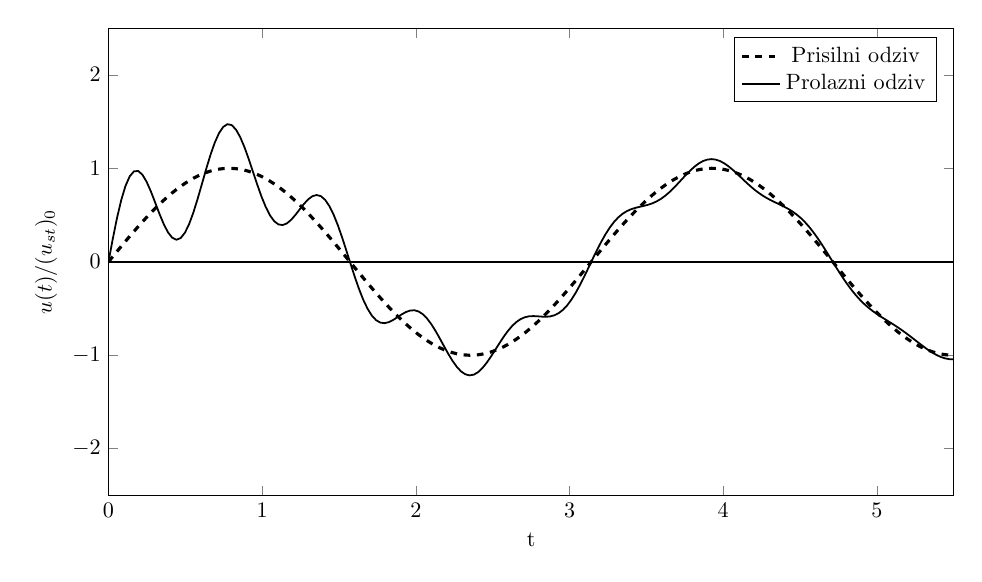
\begin{tikzpicture}[scale=0.8]
    \begin{axis} [
        height=9cm,
%        axis lines = center,
        xlabel=t,ylabel=$u(t)/(u_{st})_0$,
        ylabel near ticks, ylabel style={anchor=south},
        xmin = 0, xmax = 5.5,
        ymin = -2.5, ymax = 2.5,
        xtick = {0, 1, 2, 3, 4, 5},
        ytick = {-2,-1, 0, 1, 2},
     ]
        \addplot [
            domain=0:5.5,
            samples=200,
            color=black,
            dashed,line width=0.5mm,
        ] {sin(2*deg(x))};
        \addlegendentry{Prisilni odziv}
        \addplot [
            domain=0:5.5,
            samples=200,
            color=black,
            thick,
        ] {sin(2*deg(x))+0.7*exp(-0.05*10*x)*sin(10*deg(x))};
        \addlegendentry{Prolazni odziv}
    \draw[thick] (0,0)--(5.5,0);
    \end{axis}
\end{tikzpicture}

    \label{fig:odziv-priguseno}
    \caption{Odziv prigušenog sustava na pobudu sinusnom silom za
    $\omega/\omega_n=0.2$ i $\zeta=0.05$}
\end{figure}

Neprigušeni sustav možemo shvatiti kao poseban slučaj prigušenog sustava za slučaj
$c=0$ odnosno $\zeta=0$, pa diferencijalna jednadžba sustava postaje:
\begin{equation}\label{eq:jednadzba_gibanja_nepriguseni_nesredjeno}
	m\ddot{u}+ku=p(t)
\end{equation}
\begin{figure}[H]
    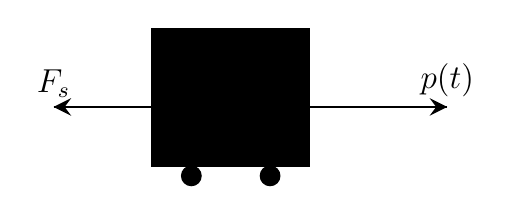
\begin{tikzpicture}
%povecaj strelice
\tikzset{myptr/.style={decoration={markings,mark=at position 1 with %
    {\arrow[scale=2,>=stealth]{>}}},postaction={decorate}}}

	%podloga
%	\draw[white, pattern=north east lines, pattern color=black] (0, 0)
%	rectangle (-0.5, 2.2);
%	\draw[thick] (0,0) -- (0, 2.2);

%	\draw[white, pattern=north east lines, pattern color=black] (0, 0) 
%	rectangle (5, -0.5);
%	\draw[thick] (0,0) -- (5,0);
	
%	\draw[white, pattern=north east lines, pattern color=black] (0, 0)
%	rectangle (-0.5, -0.5);

	%uteg
	\filldraw[fill=black] (1.5, 2) rectangle (3.5, 0.25);

	%kotaci
	\filldraw[fill=black] (2, 0.125) circle (0.125);
	\filldraw[fill=black] (3, 0.125) circle (0.125);

	%sile
	\draw[myptr] (1.5, 1) -- (0.25, 1) 
		node[pos=1, above]{\textbf{\large{$F_s$}}};
	\draw[myptr] (3, 1) -- ( 5.25, 1) 
		node[pos=1, above]{\textbf{\large{$p(t)$}}};

\end{tikzpicture}

    \label{sile-nepriguseni-ekvivalentni-sustav-sdf}
    \caption{Dijagram sila linearnog neprigušenog sustava s jednim stupnjem slobode}
\end{figure}

Rješenje jednadžbe gibanja možemo odrediti iz \eqref{eq:inverz_treci_korak}
određivanjem koeficijenata $A$, $B$, $C$ i $D$ za $\zeta = 0$.
\begin{align}
    A &= u(0) \label{eq:np_koef_A}\\
    B &= \frac{\dot{u}(0)}{\omega_n}-\frac{\omega/\omega_n}{1-(\omega/\omega_n)^2}\label{eq:np_koef_B}\\
    C &= \frac{p_0}{k}\frac{1}{1-(\omega/\omega_n)^2}\label{eq:np_koef_C}\\
    D &= 0\label{eq:np_koef_D}\\
    \sigma &= \omega_n\zeta=\omega_n\cdot 0=0\label{eq:np_sigma}\\
    \omega_D &= \omega_n\sqrt{1-\zeta^2}=\omega_n\sqrt{1-0}=\omega_n\label{eq:np_omega_D}
\end{align}

Uvrštavanjem \eqref{eq:np_koef_A}, \eqref{eq:np_koef_B}, \eqref{eq:np_koef_C},
\eqref{eq:np_koef_D}, \eqref{eq:np_sigma} i \eqref{eq:np_omega_D} u  \eqref{eq:inverz_treci_korak}
dobijemo rješenje diferencijalne jednadžbe pod
\eqref{eq:jednadzba_gibanja_nepriguseni_nesredjeno} 
koje glasi:
\begin{equation}
	u(t)=\underbrace{
            u(0)cos(\omega_n t)
	\left[
		\frac{\dot{u}(0)}{\omega_n}-\frac{\omega/\omega_n}{1-(\omega/\omega_n)^2}
        \right]sin(\omega_n t)\\
	}_{\text{\textbf{prolazni dio odziva}}}
        +
	\underbrace{
		\frac{1}{1-(\omega/\omega_n)^2} sin(\omega t)
	}_{\text{\textbf{prisilni dio odziva}}}
\end{equation}

\begin{figure}[H]
    \input{./grafovi/sdf/odziv-nepriguseno}
    \label{fig:odziv-nepriguseno}
    \caption{Odziv neprigusenog sustava za homogene početne uvjete i
    $\omega/\omega_n=0.2$}
\end{figure}
\newpage



    \newpage
    \section{Statički pomak}
Zanemarivanjem ubrzanja u diferencijalnoj jednadžbi pod
\eqref{eq:jednadzba_gibanja_nepriguseni_nesredjeno} dobijemo:
\begin{equation}\label{eq:vremenska_funkcija_statickog_pomaka}
	u(t)=\frac{p_0}{k}sin(\omega t)
\end{equation}

Navedena jednadžba predstavlja \textit{vremensku funkciju statičkog pomaka}. Pomak
nazivamo statičkim jer se zanemaruje dinamički utjecaj sile pobude (pretpostavlja se
spora promjena opterećenja).
Vremenska funkcija statičkog pomaka, preko Hookeovog zakona, stavlja u odnos silu 
pobude ($p_0sin(\omega t)$) i pomak sustava $u(t)$. Zanemarivanjem funkcije sinus, dobijemo
amplitudu statičkog pomaka koja je definirana slijedećom jednadžbom:
\begin{equation}
	(u_{st})_0 = \frac{p_0}{k}
\end{equation}



%    \newpage
    \section{Frekvencijske funkcije odziva}\label{sec:frf}
\subsection{Izvod}
Ponašanje sustava opisano je diferencijalnom jednadžbom drugog reda (u vremenskoj
domeni) koja nakon $\ltr$-transformacija postaje algebarska jednadžba u $s$ domeni (~\cite{sisbabic}).
Transformat odziva na sinusnu silu uz homogene početne uvjete glasi:
\begin{equation}
    U(s) = P(s)\cdot H(s) 
\end{equation}

Funkcija $H(s)$ naziva se prijenosnom funkcijom sustava, a definirana je kao
kvocjent odziva i pobude u $s$ domeni.
\begin{equation} \label{eq:PrijenosnaFunkcijaSustava}
    H(s)=\frac{U(s)}{P(s)} = \frac{1}{ms^2+cs+k}%\frac{\omega_n^2}{s^2+2\zeta\omega_ns+\omega_n^2}
\end{equation}

Prijenosna funkcija sustava obično sadrži dvije skupine karakterističnih točaka:
\begin{enumerate}
    \item polovi - nultočke nazivniku
    \item nule - nultočke brojnika
\end{enumerate}

Polovi predstavljaju točke u kojima prijenosna funkcija sustava divergira tj
($H(s)\to\infty$), a nule su točke u kojima vrijednost prijenosne funkcije iznosi
nula. Polovi i nule za polinom drugog stupnja mogu biti:
\begin{enumerate}
    \item dva različita realna broja
    \item jedan dvostruki realni broj
    \item jedan par kompleksno konjugiranih brojeva
\end{enumerate}

Uočimo da za slučaj prijenosne funkcije sustava pod
\eqref{eq:PrijenosnaFunkcijaSustava} nema nula, a polovi su jedan par kompleksno
konjugiranih brojeva (polovi su dobiveni izjednačavanjem polinoma u nazivniku s
nulom):
\begin{equation}
    p_{1,2} = -\sigma\pm\omega_Di
\end{equation}

Realni dio pola prikazuje stupanj prigušenja, a imaginarni dio prirodnu frekvenciju 
prigušenog titranja. Prijenosna funkcija zapisana preko polova glasi:
\begin{equation}
    H(s)=\frac{1}{(s-p_1)(s-p_2)}
%         \frac{\omega_n}{(s+\sigma+\omega_Di)(s+\sigma-\omega_Di)}=
%         \frac{\omega_n}{(s+\sigma)^2+\omega_D^2}
\end{equation}

Raspisivanjem dobijemo:
\begin{equation}
    H(s)=\frac{1}{(s+\sigma+\omega_Di)(s+\sigma-\omega_Di)}\frac{\omega_n^2}{k}
\end{equation}

I konačno tablični oblik dobijemo množenjem s $\omega_D/\omega_D$
\begin{equation}
    H(s)=\frac{1}{k}\frac{\omega_n^2}{\omega_D}\frac{\omega_D}{(s+\sigma^2)+\omega_D^2}
\end{equation}

Poseban slučaj prijenosne funkcije sustava, za slučaj $s=\omega i$, naziva se
\textit{frekvencijska funkcija odziva} (~\cite{sisbabic}) i glasi:
\begin{equation} \label{eq:frf_nesredjeno}
    H(\omega i) = \frac{H(\omega i)}{P(\omega i)}
                = \frac{1}{-\omega^2 m + i\omega c + k}\frac{1/k}{1/k}
                = \frac{1}{k}\frac{1}{1-(\omega/\omega_n)^2+2\zeta(\omega/\omega_n)i}
\end{equation}

Član $1/k$ možemo zanemariti jer je uračunat u amplitudu statičkog pomaka $(u_{st})_0=p_0/k$,
pa je konačni oblik frekvencijske funkcije odziva:
\begin{equation}\label{eq:frf_sredjeno}
    H(\omega) = \frac{1}{\left(1-(\omega/\omega_n)^2\right)+\left(2\zeta\omega/\omega_n\right)i}
\end{equation}

Frekvencijska funkcija odziva $H(\omega)$ je funkcija argumenta $\omega$, odnosno promjenom
frekvencije pobude, mjenja se i njezina vrijednost, te je redovito je kompleksna (~\cite{sisbabic}).
Jednadžbu pod \eqref{eq:frf_sredjeno} možemo rastaviti na realni i imaginarni dio.
Rastav na realni i imaginarni dio prikazan je u nastavku.
\begin{alignat}{2}
    &\text{Realni dio} & H_r &= \frac{1-(\omega/\omega_n)^2}{(1-(\omega/\omega_n)^2)^2+(2\zeta\omega/\omega_n)^2}
        \label{eq:realni_dio_frf}\\
    &\text{Imaginarni dio}\quad & H_i &=\frac{2\zeta(\omega/\omega_n)}{(1-(\omega/\omega_n)^2)^2+(2\zeta\omega/\omega_n)^2}
        \label{eq:imaginarni_dio_frf}
\end{alignat}

Jednadžba pod \eqref{eq:frf_sredjeno} zapisana preko realnog i imaginarnog dijela
glasi:
\begin{equation}\label{eq:frf_pravokutni}
    \begin{split}
        H(\omega) &= H_r - H_ii  \\
              &= \frac{1-(\omega/\omega_n)^2}{(1-(\omega/\omega_n)^2)^2+(2\zeta\omega/\omega_n)^2}
              -\frac{2\zeta(\omega/\omega_n)}{(1-(\omega/\omega_n)^2)^2+(2\zeta\omega/\omega_n)^2}i
    \end{split}
\end{equation}

Funkciju \eqref{eq:frf_sredjeno} se može prikazati i u trigonometrijskom obliku.
Općenito, kompleksni broj se prikazuje u trigonometrijskom obliku na slijedeći
način:
\begin{equation}\label{eq:trig_zapis_kompleksni_br}
    R=|R|e^{i\phi} = |R|(\cos(\phi)+i\sin(\phi))
\end{equation}
gdje je $|R|$ apsolutna vrijednost ili norma kompleksnog broja, a $\phi$ kut kojega 
kompleksni vektor zatvara s realnom osi.
Stoga je očito da je za navedeni prikaz potrebno je odrediti normu kompleksnog
broja frekvencijske funkcije odziva te kut koji zatvara s realnom osi. Norma je 
zadana Pitagorinim poučkom, dakle:
\begin{equation}\label{eq:magnitudniSpektar}
    |H(\omega)|=\sqrt{(H_r^2+H_i^2)}
               =\frac{1}{\sqrt{(1-(\omega/\omega_n)^2)^2+(2\zeta(\omega/\omega_n))^2}}
\end{equation}

Kut koji kompleksni vektor zatvara s realnom osi moguće je odrediti slijedećom
jednadžbom:
\begin{equation}\label{eq:fazniSpektar}
    \phi(\omega)= \left|\arctan\left(\frac{H_i}{H_r}\right)\right| 
                = \left|\arctan\left(\frac{2\zeta(\omega/\omega_n)}
                        {1-(\omega/\omega_n)^2}\right)\right|
\end{equation}

Prikazana u trigonometrijskom obliku, frekvencijsku funkciju odziva potrebno je
rastaviti na normu koja je definirana jednadžbom \eqref{eq:magnitudniSpektar} i
na fazni kut koji je definiran jednadžbom \eqref{eq:fazniSpektar}.
\textbf{Napomena:} jednadžba \eqref{eq:fazniSpektar} stavljena je u apsolutnu
vrijednost zato što će se negativni predzak (kašnjenje) ili pozitivni predznak
uračunati naknadno, no više o tome u slijedećem poglavlju.

    \newpage
    \subsection{Zapis prisilnog dijela odziva}
Prisilni dio odziva definiran definiran je jednadžbom prikazanom u nastavku:
\begin{equation}\label{eq:samo_prisilni}
    u(t)=C\sin(\omega t) + D\cos(\omega t)
\end{equation}

Prisilni odziv pod \eqref{eq:samo_prisilni} možemo zapisati u obliku $u_0\sin(\omega t
- \phi)$ 
korištenjem slijedećeg trigonometrijskog identiteta:
\begin{equation}\label{eq:prisilni_dio_odziva}
    u_0\sin(\omega t - \phi) = C\sin(\omega t) + D\cos(\omega t)
\end{equation}

Gdje je:
\begin{alignat}{2}
    &\text{Amplituda dinamičkog pomaka} & u_0 &= \sqrt{C^2+D^2}\label{eq:u_0-izvod-prvo}\\
    &\text{Kašnjenje u fazi} & \phi &= \arctan{-\frac{D}{C}}\label{eq:fi-izvod}
\end{alignat}

Raspisivanjem formule pod \eqref{eq:u_0-izvod-prvo} dobijemo:
\begin{equation}\label{eq:u_0-izvod-raspisano}
    u_0 = \frac{p_0}{k}\frac{1}{\sqrt{(1-(\omega/\omega_n)^2)^2+(2\zeta\omega/\omega_n)^2}}
        = \frac{(u_{st})_0}{\sqrt{(1-(\omega/\omega_n)^2)^2+(2\zeta\omega/\omega_n)^2}}
\end{equation}

Definiramo dinamički koeficijent pomaka ili koeficijent povećanja pomaka ($R_d$) kao omjer
amplitude dinamičkog i statičkog pomaka.
\begin{equation}\label{eq:R_d-izvod-konacno}
    R_d = \frac{u_0}{(u_{st})_0}=\frac{1}{\sqrt{(1-(\omega/\omega_n)^2)^2+(2\zeta\omega/\omega_n)^2}}
\end{equation}

Fazni kut $\phi$ dobijemo raspisivanjem izraza pod \eqref{eq:fi-izvod} te dobijemo:
\begin{equation}\label{eq:fi-izvod-konacno}
    \phi = \arctan{\frac{2\zeta(\omega/\omega_n)}{1-(\omega/\omega_n)^2}}
\end{equation}

Uvrštavanjem \eqref{eq:R_d-izvod-konacno} i \eqref{eq:fi-izvod-konacno} u
\eqref{eq:prisilni_dio_odziva} dobijemo:
\begin{equation}
    u(t) = \frac{p_0}{k}R_d\sin(\omega t - \phi) = (u_{st})_0R_d\sin(\omega t - \phi)
\end{equation}

Uočimo da je jednadžba pod \eqref{eq:R_d-izvod-konacno} ista kao i jednadžba
magnitudnog spektra frekvencijske funkcije odziva. Isto tako, uočimo i da je jednadžba
pod \eqref{eq:fi-izvod-konacno} ista kao i jednadžba faznog spektra frekvencijske
funkcije odziva. Nadalje, prisilni dio odziva je sinusoida isto kao i pobuda.
\par
 
Stoga možemo reći da frekvencijska funkcija odziva definira odnos između pobude i
odziva. Taj odnos je kompleksan jer je opisan magnitudnim i faznim spektrom
kompleksne funkcije definirane u $s$ domeni. Drugim riječima, frekvencijska funkcija
odziva nas upućuje na slijedeća svojstva (prisilnog) odziva:
\begin{enumerate}
    \item Frekvencija odziva biti će jednaka frekvenciji pobude.
    \item Amplituda odziva biti će skalirana amplituda statičkog pomaka. Prisjetimo
        se da je amplituda statičkog pomaka u izravnoj vezi sa amplitudom sile pobude.
    \item Odziv će zaostajati u fazi za pobudom. 
\end{enumerate}

Skaliranje amplitude statičkog pomaka $(u_{st})_0$ definirano je \textit{dinamičkim
koeficijentom} $R_d$. Navedeni koeficijent je konkretna vrijednost magnitudnog
spektra frekvencijske funkcije odziva za određenu frekvenciju $\omega$. Analogno
tome, kašnjenje u fazi definirano je faznim kutom koji je konkretna vrijednost
faznog spektra frekvencijske funkcije odziva.

\subsubsection{Alternativno zapis prisilnog dijela odziva(Za ovo i nisam baš
siguran)}
Odziv na pobudu sinusnom silom može se odrediti konvolucijom prijenosne funkcije i
funkcije pobude u vremenskoj domeni. Zadana je pobuda sinusnom silom oblika:
\begin{equation}\label{eq:pobuda_sinusnom_silom}
    p(t)=p_0e^{\alpha t} \sin(\omega t)
\end{equation}

Jednadžbu \eqref{eq:pobuda_sinusnom_silom} možemo zapisati u eksponencijalnom
obliku:
\begin{equation}\label{eq:pobuda_sinusnom_silom_eksponencijalni}
    p(t)=-\frac{1}{2}p_0i(e^{(\alpha+i\omega)t}-e^{(\alpha-i\omega)t})
\end{equation}

Uvodimo:
\begin{align}
    s  &= \alpha + i\omega \label{eq:s_normalno}\\
    s^* &= \alpha - i\omega \label{eq:s_konjugirano}
\end{align}
Uvrštavanjem \eqref{eq:s_normalno} i \eqref{eq:s_konjugirano} u
\eqref{eq:pobuda_sinusnom_silom_eksponencijalni} dobijemo:
\begin{equation}\label{eq:pobuda_sinusnom_silom_konacno}
    p(t) = -\frac{1}{2}p_0(e^{st}-e^{s^*t})
\end{equation}

Prijenosna funkcija sustava (s izlučenim članom $1/k$) zadana je u obliku $1/k
h(t)$. Izračun odziva je prikazan u nastavku:
\[
    u(t) = \frac{1}{k}(h*p)(t) 
         = \frac{1}{k}\int_0^\infty h(t-\tau)p(\tau)d\tau
\]

Uvodi se supstitucija $\lambda=t-\tau$.
\[
    u(t) = \frac{1}{k}\int_0^\infty h(\lambda)p(t-\lambda)d\lambda
         = \frac{1}{k}\int_0^\infty h(\lambda)\left[
             -\frac{1}{2}p_0i\left(e^{st-s\lambda}-e^{s^*t-s^*\lambda}\right)
             \right]d\lambda
\]
Raspisivanjem i sređivanjem dobijemo:
\begin{equation}\label{eq:prisilni_transformacija_prijenosne}
    u(t) = -\frac{1}{2}\frac{p_0}{k}i \left[
                e^{st}
                \underbrace{
                    \int_0^\infty h(\lambda)e^{-s\lambda}d\lambda
                }_{\text{\textbf{$I)$}}}
                -e^{s^*t}
                \underbrace{
                    \int_0^\infty h(\lambda)e^{-s^*\lambda}d\lambda
                }_{\text{\textbf{$II)$}}}
        \right]
\end{equation}
Uočimo da integrali označeni s $I)\text{ i } II)$ predstavljaju Laplaceovu
transformaciju prijenosne funkcije sustava pa izraz pod \eqref{eq:prisilni_transformacija_prijenosne}
postaje:
\begin{equation}\label{eq:prisilni_transformacija_prijenosne_kk}
    u(t)=-\frac{1}{2}\frac{p_0}{k}i(e^{st}H(s)-e^{s^*t}H(s))
\end{equation}

Varijabla $s^*$ je kompleksno konjugirana varijabla $s$, pa je funkcija
$H(s^*)$ kompleksno konjugirana funkcija $H(s)$. odnosno:
\begin{equation}\label{eq:prijenosne_odnos}
    H(s^*)=H^*(s) 
\end{equation}

Korištenjem \eqref{eq:prijenosne_odnos} jednadžba \eqref{eq:prisilni_transformacija_prijenosne_kk}
postaje:
\begin{equation}\label{eq:prisilni_transformacija_prijenosne_hk}
    u(t)=-\frac{1}{2}\frac{p_0}{k}i (e^{st}H(s)-e^{s^*t}H^*(s))
\end{equation}

Poseban slučaj je za $\alpha = 0$ odnoso $s=i\omega \text{ i } s^*=-i\omega$. Tada
prijenosne funckije sustava postaju frekvencijske funkcije odziva, a izraz pod
\eqref{eq:prisilni_transformacija_prijenosne_hk} glasi:

\begin{equation}\label{eq:prisilni_transformacija_frf}
    u(t) = -\frac{1}{2}\frac{p_0}{k}i(e^{i\omega t}H(\omega i) - e^{-i\omega t}H^*(i\omega))
\end{equation}

Frekvencijska funkcija odziva $H(\omega i)$ zadana je jednadžbom \eqref{eq:frf_pravokutni}.
Možemo uočiti da je njezin imaginarni dio negativan, što znači da je imaginarni dio
funkcije $H^*(\omega i)$ pozitivan.
\begin{figure}[H]
    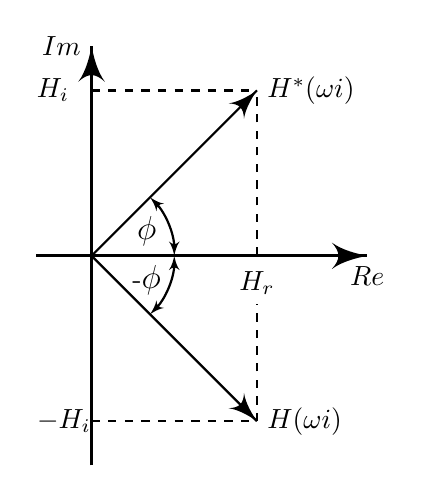
\begin{tikzpicture}[scale=0.7,>=latex']
\tikzset{strelica/.style={decoration={markings,mark=at position 1 with %
    {\arrow[scale=2,>=latex']{>}}},postaction={decorate}}}

    \draw[strelica,very thick] (0,-3.8) -- (0,3.8)
        node[pos=1,left]{$Im$};
    \draw[strelica,very thick] (-1,0) -- (5,0)
        node[pos=1,below]{$Re$};

    %H(w)
    \draw[strelica,thick] (0, 0) -- (3,-3)
        node[pos=1,right]{$H(\omega i)$};

    \draw[strelica,thick] (0,0) -- (3,3)
        node[pos=1,right]{$H^*(\omega i)$};

    \draw[dashed,thick] (3,-3) -- (3,3);
    \draw[dashed,thick] (0, 3) -- (3,3);
    \draw[dashed,thick] (0,-3) -- (3,-3);

    \node[rectangle,fill=white] at (3,-0.5) {$H_r$};
    \node at (-0.5,-3) {$-H_i$};
    \node at (-0.7, 3) {$H_i$};

    %-fi
    \draw [<->,thick] (1.5,0) arc [start angle=0, end angle=-45, radius=1.5];
    \node at (1,-0.45) {-\large{$\phi$}};

    %fi
    \draw [<->,thick] (1.5,0) arc [start angle=0, end angle= 45, radius=1.5];
    \node at (1,0.45) {\large{$\phi$}};

\end{tikzpicture}

    \caption{Shematski prikaz funkcija $H(\omega i) \text{ i }H^*(\omega i)$ u
    Gaussovoj ravnini}
    \label{fig:frf-gauss}
\end{figure}

Modul funkija $H(\omega)$ i $H^*(\omega)$ je isti a definiran je jednadžbom
\eqref{eq:magnitudniSpektar} a fazni kut jednadžbom \eqref{eq:fazniSpektar}. Sa
slike \ref{fig:frf-gauss} vidljivo je da je kut $\phi$ što ga zatvara $H(\omega)$ s
realnom osi negativan, a kut što ga zatvara $H^*(\omega)$ s realnom osi pozitivan.
Trigonometrijski zapisi funkcija $H(\omega) \text{ i } H^*(\omega)$ dati su u
nastavku.
\begin{align}
    H(\omega) &= |H(\omega)|e^{-i\phi} \label{eq:trig_zapis}\\
    H^*(\omega) &= |H(\omega)|e^{i\phi} \label{eq:trik_zapis_hk}\\ %hk- h-kompleksno konjugiran
\end{align}

Uvrštavanjem \eqref{eq:trig_zapis} i \eqref{eq:trig_zapis_kk} u \eqref{eq:prisilni_transformacija_prijenosne_hk}
dobijemo:
\begin{equation}
    u(t)=-\frac{1}{2}\frac{p_0}{k}i|H(\omega)|(e^{i\omega t}e^{-i\phi}-e^{-i\omega t}e^{i\phi})
        =-\frac{1}{2}\frac{p_0}{k}i|H(\omega)|(2i\sin(\omega t -\phi))
\end{equation}

Te konačno:
\begin{equation}\label{eq:prisilni_alternativno_rjesenje}
    u(t)=\frac{p_0}{k}|H(\omega)|\sin(\omega t - \phi)
\end{equation}
Jednadžba \eqref{eq:prisilni_alternativno_rjesenje} predstavlja prisilni dio odziva.

Definiramo dinamički koeficijent pomaka ili koeficijent povećanja pomaka ($R_d$) kao omjer
amplitude dinamičkog i statičkog pomaka.
\begin{equation}\label{eq:R_d-izvod-konacno}
    R_d = \frac{u_0}{(u_{st})_0}=\frac{1}{\sqrt{(1-(\omega/\omega_n)^2)^2+(2\zeta\omega/\omega_n)^2}}
\end{equation}

Uočimo da su jednadžbe \eqref{eq:R_d-izvod-konacno} i \eqref{eq:frf_sredjeno} iste,
odnosno funkcija ovisnost dinamičkog faktora $R_d$ o omjeru frekvencija
$\omega/\omega_n$ odgovara magnitudnom spektru frekvencijske funkcije odziva. Stoga
jednadžbu pod \eqref{eq:prisilni_alternativno_rjesenje} možemo zapisati kao:
\begin{equation}\label{eq:prisilni_alternativno_rjesenje_Rd}
    u(t)=\frac{p_0}{k}R_d\sin(\omega t - \phi)
\end{equation}

Iz \eqref{eq:prisilni_alternativno_rjesenje} i \eqref{eq:prisilni_alternativno_rjesenje_Rd}
možemo definirati fizikalnu interpretaciju frekvencijske funkcije odziva.
Dakle, frekvencijska funkcija odziva definira odnos između pobude i
odziva. Taj odnos je kompleksan jer je opisan magnitudnim i faznim spektrom
kompleksne funkcije definirane u $s$ domeni. Drugim riječima, frekvencijska funkcija
odziva nas upućuje na slijedeća svojstva (prisilnog) odziva:
\begin{enumerate}
    \item Frekvencija odziva biti će jednaka frekvenciji pobude ($\omega$).
    \item Amplituda odziva biti će skalirana amplituda statičkog pomaka. Prisjetimo
        se da je amplituda statičkog pomaka u izravnoj vezi sa amplitudom sile pobude.
    \item Odziv će zaostajati u fazi za pobudom. 
\end{enumerate}

Skaliranje amplitude statičkog pomaka $(u_{st})_0$ definirano je \textit{dinamičkim
koeficijentom} $R_d$. Navedeni koeficijent je konkretna vrijednost magnitudnog
spektra frekvencijske funkcije odziva za određenu frekvenciju $\omega$. Analogno
tome, kašnjenje u fazi definirano je faznim kutom koji je konkretna vrijednost
faznog spektra frekvencijske funkcije odziva.


    \newpage
    \subsection{Grafički prikaz frekvencijske funkcije odziva}
Zbog toga što frekvencijska funkcija pomaka definira uvećanje amplitude statičkog
pomaka (dinamički koeficijent pomaka) i fazno zaostajanje odziva za pobudom od posebnog 
su nam interesa kut i intenzitet frekvencijske funkcije odziva (polarni zapis).
\par

Za konstantan $\omega_n$ vrijednosti funkcija definiranih jednadžbama 
\eqref{eq:magnitudniSpektar} i \eqref{eq:fazniSpektar} biti će za omjer
$\omega/\omega_n$, stoga taj omjer možemo postaviti i kao argument navedenih
funkcija. 
\begin{equation}\label{eq:magnitudniSpektarZaOmjer}
    R_d = \left|H\left(\frac{\omega}{\omega_n}\right)\right|=
        \frac{1}{\sqrt{((1-(\omega/\omega_n)^2)^2+(2\zeta(\omega/\omega_n))^2}}
\end{equation}

\begin{equation}\label{eq:fazniSpektarZaOmjer}
    \phi\left(\frac{\omega}{\omega_n}\right)=
        \arctan\left(\frac{2\zeta(\omega/\omega_n)}{1-(\omega/\omega_n)}\right)
\end{equation}

\begin{figure}[H]
    \begin{subfigure}{1\textwidth}
        \input{./grafovi/sdf/rd-priguseno}
    \end{subfigure}
    \vfill
    \begin{subfigure}{1\textwidth}
        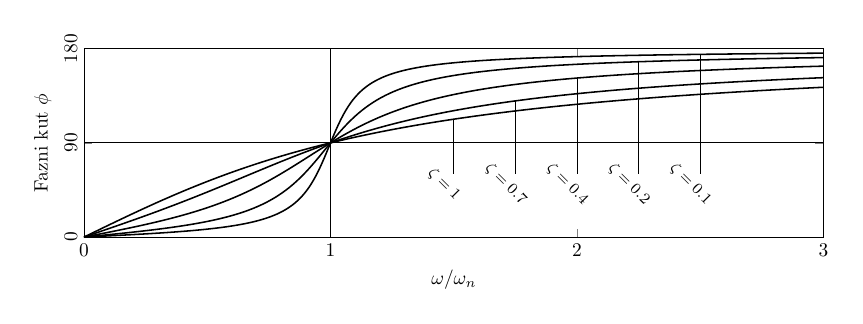
\begin{tikzpicture}[scale=0.7]
	\begin{axis} [
		height=5cm,
		ylabel = Fazni kut $\phi$, 
		xlabel = $\omega/\omega_n$,
		xmin = 0,
		xmax = 3,
		ymin = 0,
		ymax = 180,
		xtick = {0,1,2,3}, 
		ytick = {0,90,180}, yticklabel style={rotate=90},
	]

            \foreach \i in {1, 0.7, 0.4, 0.2, 0.1}
            {
                \addplot [
                    domain=0:1,
                    samples=200,
                    color=black,
                    thick
                ]{atan((2*x*\i)/(1-x^2))};
            }

            \foreach \i in {1, 0.7, 0.4, 0.2, 0.1}
            {
                \addplot [
                    domain=1.001:3,
                    samples=200,
                    color=black,
                    thick
                ]{180+atan((2*x*\i)/(1-x^2))};
            }
            \draw[thin](1.5,{180+atan((2*1.5*1)/(1-1.5^2))}) -- (1.5, 60)
                node[pos=1,rotate=-45,below] {\footnotesize{$\zeta=1$}};
            \draw[thin](1.75,{180+atan((2*1.75*0.7)/(1-1.75^2))}) -- (1.75, 60)
                node[pos=1,rotate=-45,below] {\footnotesize{$\zeta=0.7$}};
            \draw[thin](2,{180+atan((2*2*0.4)/(1-2^2))}) -- (2, 60)
                node[pos=1,rotate=-45,below] {\footnotesize{$\zeta=0.4$}};
            \draw[thin](2.25,{180+atan((2*2.25*0.2)/(1-2.25^2))}) -- (2.25, 60)
                node[pos=1,rotate=-45,below] {\footnotesize{$\zeta=0.2$}};
            \draw[thin](2.5,{180+atan((2*2.5*0.1)/(1-2.5^2))}) -- (2.5, 60)
                node[pos=1,rotate=-45,below] {\footnotesize{$\zeta=0.1$}};



        \draw[thin](1,0)--(1,180);
        \draw[thin](0,90) -- (3,90);
        \end{axis}
\end{tikzpicture}

    \end{subfigure}
    \caption{Dinamički koeficijent i fazni kut za prigušeni sustav pri harmonijskoj
    pobudi}
    \label{fig:frf-priguseno}
\end{figure}

Intenzitet frekvencijske funkcije odziva prikazuje funkcijsku ovisnost
dinamičkog koeficijenta $R_d$ o omjeru frekvencije pobude i prirodne frekvencije za
određeno prigušenje. Analogno tome fazni kut frekvencijske funkcije odziva
prikazuje kašnjenje u fazi za pobudom u ovisnosti o omjeru frekvencija 
$\omega/\omega_n$ za određeni faktor relativnog prigušenja.
\par

Za neprigušeno titranje, funkcije faznoga kuta i dinamičkog koeficijenta pomaka prikazane 
su u nastavku.
\begin{equation}\label{eq:fazniSpektarNepriguseno}
    \phi\left(\frac{\omega}{\omega_n}\right)=
        \arctan\left(\frac{0}{1-(\omega/\omega_n)}\right)
\end{equation}
\begin{equation}\label{eq:magnitudniSpektarNepriguseno}
    R_d=\left|H\left(\frac{\omega}{\omega_n}\right)\right|=
        \frac{1}{\sqrt{((1-(\omega/\omega_n)^2)^2+(2\cdot 0(\omega/\omega_n))^2}} =
        \frac{1}{|1-(\omega/\omega_n)^2|}
\end{equation}

Iz formule \eqref{eq:fazniSpektarNepriguseno} očito je da za neprigušeno titranje
postoje tri vrijednosti faznog kuta koje ovise o izrazu u nazivniku. Vrijednosti
faznog kuta prikazane su u nastavku:
\[
    \phi = \begin{dcases*}
            0\degree   & za $1-(\omega/\omega_n)^2 > 0$\\ % & $\omega < \omega_n$\\
            90\degree  & za $1-(\omega/\omega_n)^2 = 0$\\ % & $\omega = \omega_n$\\
            180\degree & za $1-(\omega/\omega_n)^2 < 0$\\ % & $\omega > \omega_n$\\
        \end{dcases*}
\]

\begin{figure}[H]
    \begin{subfigure}{1\textwidth}
        \begin{tikzpicture}[scale=0.7]
    \begin{axis} [
        ylabel = Dinamički koeficijent $R_d$,
        xlabel = $\omega/\omega_n$,
        xmin = 0, xmax = 3,
        ymin = 0, ymax = 6,
        xtick = {0, 1, 2, 3},
        ytick = {1, 2, 3, 4, 5, 6},
     ]

        \draw[thin] (1,0) -- (1,6);
        \draw[thin] (0,1) -- (3,1);
    \foreach \i in {1, 0.7, 0.4, 0.2, 0.1}
        {
            \addplot [
                domain=0:3,
                samples=200,
                color=black,
                thin,
            ]{1/abs(1-x^2)};
        }
    \end{axis}
\end{tikzpicture}

    \end{subfigure}
    \vfill
    \begin{subfigure}{1\textwidth}
        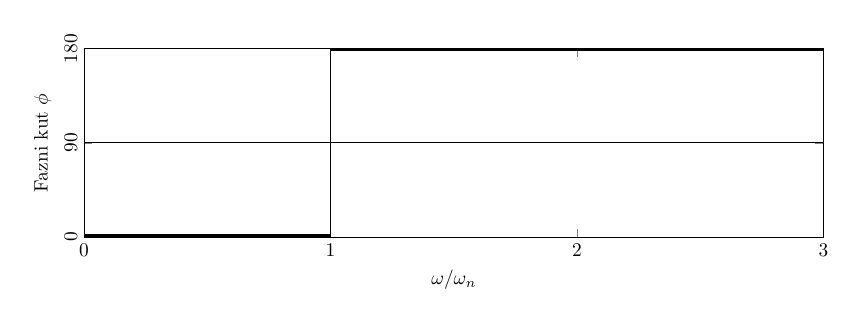
\begin{tikzpicture}[scale=0.7]
	\begin{axis} [
		height=5cm,
		ylabel = Fazni kut $\phi$, 
		xlabel = $\omega/\omega_n$,
		xmin = 0, xmax = 3,
		ymin = 0, ymax = 180,
		xtick = {0,1,2,3}, 
		ytick = {0,90,180}, yticklabel style={rotate=90},
	]
            \draw[thin] (0,90) -- (3,90);
            \draw[thin] (1,0)  -- (1,180);

        \addplot [
            domain=0:1,
            samples=200,
            color=black,
            line width=1mm,
        ]{atan((2*x*0)/(1-x^2))};
        \addplot [
                    domain=1.001:3,
                    samples=200,
                    color=black,
                    line width=1mm, 
       ]{180+atan((2*x*0)/(1-x^2))};
        \end{axis} 
\end{tikzpicture}

    \end{subfigure}
    \caption{Dinamički koeficijent i fazni pomak za neprigušeni sustav pri
    harmonijskoj pobudi}
    \label{fig:frf-nepriguseno}
\end{figure}
\newpage

Analizirajući krivulje sa \eqref{fig:frf-priguseno} i \eqref{fig:frf-nepriguseno} 
navedene grafove možemo podijeliti na tri područja (~\cite{chopra2011}):
\begin{enumerate}
    \item Područje kontrolirano krustošću - za slučaj spore promjene opterećenja
        ($\omega/\omega_n<<1$ - lijevo na grafu) utjecaj prigušenja je neznatan
        (krivulje za različita prigušenja su jako bliske) a dinamički utjecaj je mali, 
        tj. $R_d \approx 1$ što znači da je amplituda prisilnog odziva približno jednaka
        amplitudi statičkog pomaka, pa amplitudu prisilnog odziva možemo
        aproksimirati slijedećom jednadžbom:
        \begin{equation}\label{eq:frf_prvi_sektor}
            u_0\simeq(u_{st})_0=\frac{p_0}{k}
        \end{equation}
        Fazni kut je približno $0\degree$ pa su pobuda i odziv u fazi.

    \item Područje kontrolirano prigušenjem - Za slučaj $\omega/\omega_n\simeq 1$,
        izražen razmak između krivulja nalaže najeveći utjecaj prigušenja na
        vrijednost dinamičkog faktora, a samim time i na ukupnu amplitudu prisilnog
        odziva. Dinamički faktor $R_d$, u navedenom intervalu, postiže najveće
        vrijednosti a u slučaju $\zeta=0$ $R_d$ je neograničen (teži u beskonačno). 
        Dominantni član izraza \eqref{eq:magnitudniSpektarZaOmjer} je
        $2\zeta(\frac{\omega}{\omega_n})$, a aproksimacija amplitude prisilnog
        odziva glasi: 
        \begin{equation}\label{eq:frf_rezonanca}
            u_0=\frac{(u_{st})_0}{2\zeta}=\frac{p_0}{c\omega_n}
        \end{equation}

        Fazni kut za sva prigušenja iznosi 90\degree. 

    \item Područje kontrolirano masom - Za slučaj brze promjene opterećenja
        $\omega/\omega_n>>1$ utjecaj prigušenja je zanemariv jer su krivulje vrlo
        bliske. Dinamički faktor $R_d$ teži u nulu, što znači da je ukupna amplituda
        prisilnog odziva manja od amplitude statičkog pomaka. Dominantni član jednadžbe 
        \eqref{eq:magnitudniSpektar} jest $(\omega/\omega_n)^4$ što znači
        da jednadžbu pod \eqref{eq:magnitudniSpektarZaOmjer} možemo aproksimirati na 
        slijedeći način:
        \[
            H(\omega/\omega_n)\simeq \frac{\omega_n^2}{\omega^2}
        \]

        Prema tome, amplituda prisilnog odziva glasi:
        \begin{equation}\label{eq:frf_treci_sektor}
            u_0=(u_{st})_0\left(\frac{\omega_n}{\omega}\right)^2=\frac{p_0}{m\omega^2}
        \end{equation}
        
        U ovom slučaju ($\omega/\omega_n >> 1$), fazni kut je približno 180\degree,
        što znači da su pobuda i odziv izvan faze
\end{enumerate}




    \newpage
    \subsection{Dinamički koeficijenti odziva (pomaka, brzine i ubrzanja)}
U prethodnim poglavljima, prisilni dio odziva je prikazan kao vremenska funkcija pomaka
pri čemu je njegova amplituda jednaka statičkom pomaku skaliranom dinamičkim
koeficijentom pomaka $R_d$. Osim vremenskom funkcijom pomaka, odziv sustava potrebno
je opisati i vremenskim funkcijama brzine i ubrzanja.

Deriviranjem vremenske funkcije pomaka po vremenu dobijemo vremensku funkciju brzine (~\cite{chopra2011}):
    \begin{align}
        \frac{\dot{u}(t)}{(u_{st})_0} &= 
            \omega R_d\cos(\omega t - \phi)\frac{\omega_n}{\omega_n}\notag\\
        \frac{\dot{u}(t)}{\omega_n p_0/k} &= 
            \frac{\omega}{\omega_n}R_d\cos(\omega t-\phi)\label{eq:derivacijaFaktorPomaka}\\
        \frac{\dot{u}(t)}{p_0/\sqrt{km}} &=
            R_v\cos(\omega t-\phi)\label{eq:dinamickiFaktorBrzine}
    \end{align}
Gdje je:
\begin{table}[H]
    \begin{tabular}{r l}
        $R_v$ & Dinamički koeficijent brzine\\
    \end{tabular}
\end{table}

Iz jednadžbi pod \eqref{eq:derivacijaFaktorPomaka} i \eqref{eq:dinamickiFaktorBrzine}
slijedi relacija:
\begin{equation}\label{eq:R_v}
    \frac{\dot{u}(0)}{p_0/\sqrt{km}}=R_v=\left(\frac{\omega}{\omega_n}\right)R_d
\end{equation}

Analogno tome, dobije se i dinamički faktor ubrzanja koji glasi:
\begin{equation}\label{eq:R_a}
    \frac{\ddot{u}(t)}{p_0/m}=-R_a=-\frac{\omega}{\omega_n}R_v
        =-\left(\frac{\omega}{\omega_n}\right)^2R_d
\end{equation}

Gdje je:
\begin{table}[H]
    \begin{tabular}{r l}
        $R_a$ & Dinamički koeficijent ubrzanja\\
    \end{tabular}
\end{table}

\begin{figure}[H]
    \begin{subfigure}{1\textwidth}
    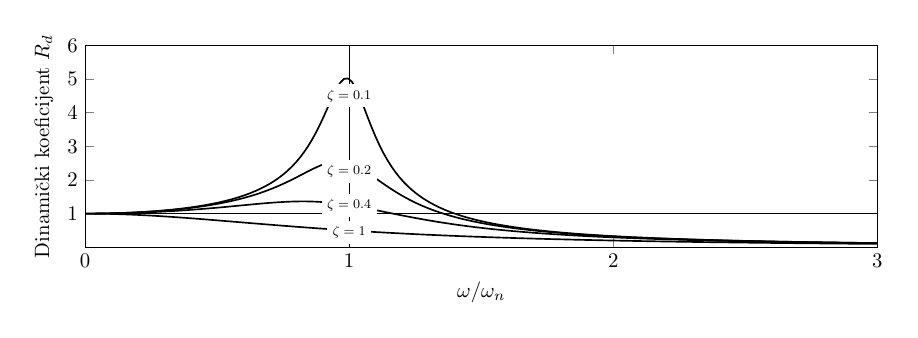
\begin{tikzpicture}[scale=0.75]
    \begin{axis} [
        height=5cm,
        ylabel = Dinamički koeficijent $R_d$,
        xlabel = $\omega/\omega_n$,
        xmin = 0, xmax = 3,
        ymin = 0, ymax = 6,
        xtick = {0, 1, 2, 3},
        ytick = {1, 2, 3, 4, 5, 6},
     ]

        \draw[thin] (1,0) -- (1,6);
        \draw[thin] (0,1) -- (3,1);
    \foreach \i in {1, 0.4, 0.2, 0.1}
        {
            \addplot [
                domain=0:3,
                samples=200,
                color=black,
                thick,
            ]{1/((1-x^2)^2+(2*\i*x)^2)^0.5};
        }
    \pgfplotsinvokeforeach{1, 0.2, 0.1}
        {
            \node[rectangle,fill=white,scale=0.8] at 
                (1,{(1-0.1)/(2*#1)}) {\footnotesize{$\zeta=#1$}};
        }
    \pgfplotsinvokeforeach{0.4}
        {
            \node[rectangle,fill=white,scale=0.8] at 
                (1,{1/(2*#1)}) {\footnotesize{$\zeta=#1$}};
        }

    \end{axis}
\end{tikzpicture}
\end{subfigure}
\vfill
\begin{subfigure}{1\textwidth}
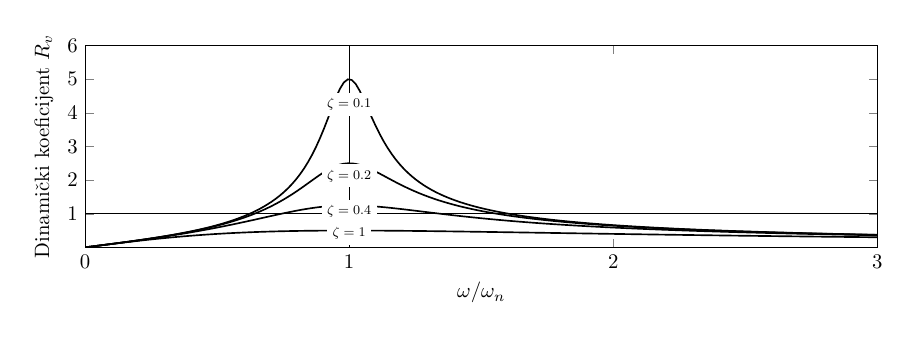
\begin{tikzpicture}[scale=0.75]
    \begin{axis} [
        height=5cm,
        ylabel = Dinamički koeficijent $R_v$,
        xlabel = $\omega/\omega_n$,
        xmin = 0, xmax = 3,
        ymin = 0, ymax = 6,
        xtick = {0, 1, 2, 3},
        ytick = {1, 2, 3, 4, 5, 6},
     ]

        \draw[thin] (1,0) -- (1,6);
        \draw[thin] (0,1) -- (3,1);
    \foreach \i in {1, 0.4, 0.2, 0.1}
        {
            \addplot [
                domain=0:3,
                samples=200,
                color=black,
                thick,
            ]{x/((1-x^2)^2+(2*\i*x)^2)^0.5};
        }
    \pgfplotsinvokeforeach{1, 0.2, 0.1,0.4}
        {
            \node[rectangle,fill=white,scale=0.8] at 
                (1,{(1-0.15)/(2*#1)}) {\footnotesize{$\zeta=#1$}};
        }
    \pgfplotsinvokeforeach{}
        {
            \node[rectangle,fill=white,scale=0.8] at 
                (1.1,{1.1/(2*#1)}) {\footnotesize{$\zeta=#1$}};
        }

    \end{axis}
\end{tikzpicture}
\end{subfigure}
\vfill
\begin{subfigure}{1\textwidth}
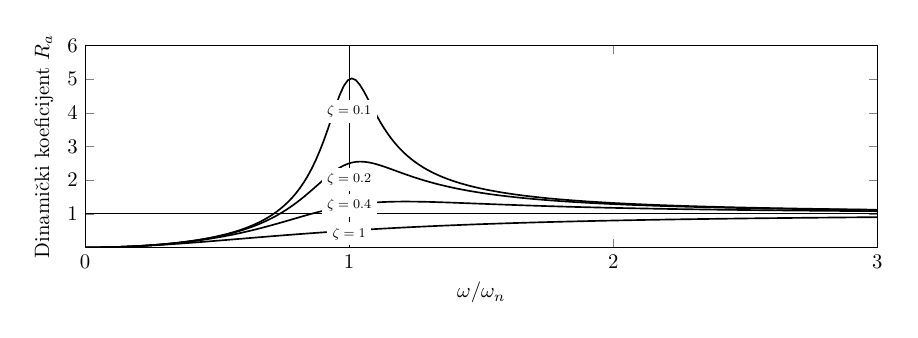
\begin{tikzpicture}[scale=0.75]
    \begin{axis} [
        height=5cm,
        ylabel = Dinamički koeficijent $R_a$,
        xlabel = $\omega/\omega_n$,
        xmin = 0, xmax = 3,
        ymin = 0, ymax = 6,
        xtick = {0, 1, 2, 3},
        ytick = {1, 2, 3, 4, 5, 6},
     ]

        \draw[thin] (1,0) -- (1,6);
        \draw[thin] (0,1) -- (3,1);
    \foreach \i in {1, 0.4, 0.2, 0.1}
        {
            \addplot [
                domain=0:3,
                samples=200,
                color=black,
                thick,
            ]{x^2/((1-x^2)^2+(2*\i*x)^2)^0.5};
        }
   \pgfplotsinvokeforeach{1, 0.2, 0.1}
        {
            \node[rectangle,fill=white,scale=0.8] at 
                (1,{(1-0.1)^2/(2*#1)}) {\footnotesize{$\zeta=#1$}};
        }
   \pgfplotsinvokeforeach{0.4}
        {
            \node[rectangle,fill=white,scale=0.8] at 
                (1,{1/(2*#1)}) {\footnotesize{$\zeta=#1$}};
        }
    \end{axis}
\end{tikzpicture}
\end{subfigure}

    \caption{Dinamički faktori pomaka, brzine i ubrzanja za različite vrijednosti
    $\zeta$}
    \label{fig:rd-rv-ra}
\end{figure}

%Sa slike \ref{fig:rd-rv-ra} vidljivo je da prigušenje na sva tri koeficijenta najviše
%utječe u okolini točke $\omega/\omega_n=1$. Isto tako vidljivo je da je maksimum
%dinamičkog faktora pomaka pomaknut u lijevo od vertikalnog pravca koji prolazi
%točkom $\omega/\omega_n=1$, a maksimum dinamičkog faktora ubrzanja u desno. 
%Maksimum dinamičkog faktora brzine pada na pravac $\omega/\omega_n=1$. Poslijedica
%toga je da se rezonantne frekvencije sustava na pomak, brzinu i ubrzanje razlikuju.
%Rezonantne frekvencije biti će razmatrane detaljnije u slijedećim poglavljima.

Iz \eqref{eq:R_v} i \eqref{eq:R_a} slijedi da su dinamički koeficijenti pomaka,
brzine i ubrzanja u odnosu. Navedeni odnos je prikazan je slijedećom jednadžbom.
\begin{equation}\label{eq:R_d-R_v-R_a}
    \frac{R_a}{\omega/\omega_n}=R_v=\frac{\omega}{\omega_n}R_d 
\end{equation}
Iz navedene jednadžbe slijedi da je poznavanjem jedne od veličina $R_d, R_v 
\text{ ili } R_a$ moguće dobiti preostale dvije. Zbog toga što postoji odnos
između dinamičkih koeficijenata pomaka, brzine i ubrzanja opisan jednadžbom 
\eqref{eq:R_d-R_v-R_a}, moguće je sve tri navedene veličine prikazati u jednom
grafu.

Takav graf se sastoji od četiri logaritamske skale:
\begin{enumerate}
    \item horizontalne logaritamske skale koja prikazuje omjer frekvencije pobude i 
        prirodne frekvencije sustava 
    \item vertikalne logaritamske skale koja prikazuje \textit{dinamički koeficijent brzine
        $R_d$}
    \item modificirane logaritamske skale nagnute pod kutem od $+45\degree$ koja prikazuje
        \textit{dinamički koeficijent ubrzanja $R_a$}
    \item modificirane logaritamske skale nagnute pod kutem od $-45\degree$ koja prikazuje
        \textit{dinamički koeficijent pomaka $R_d$}
\end{enumerate}

\begin{figure}[H]
    \pgfplotsset{
    every axis/.append style={
        line width=0.8pt,
        tick style={line width=0.8pt, color=black}
    }
}
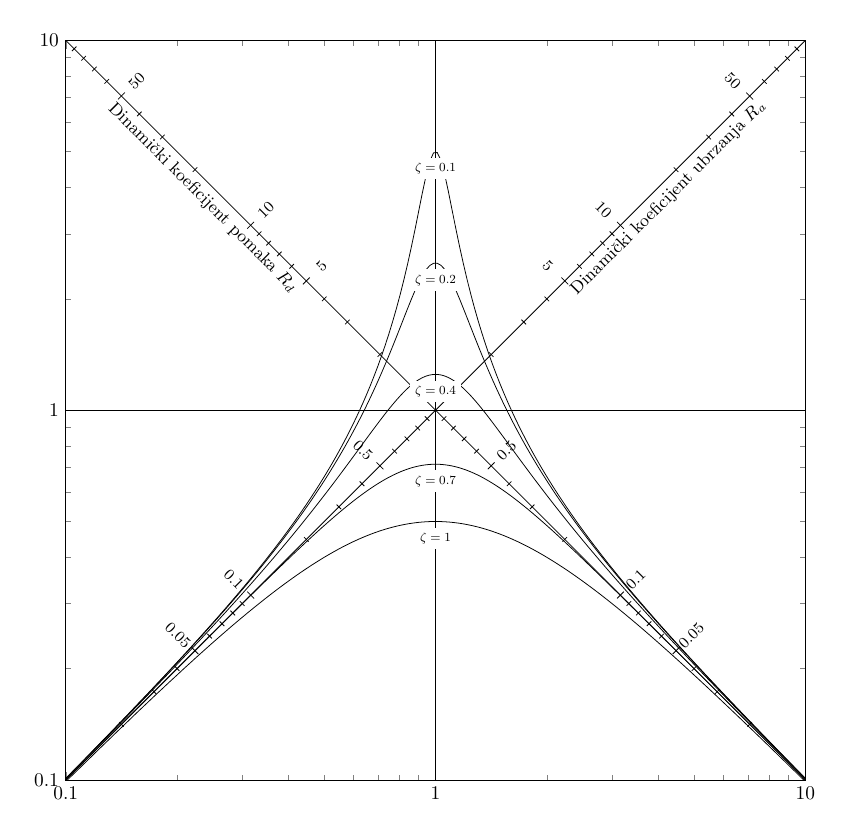
\begin{tikzpicture}[scale=0.7]
    \begin{loglogaxis} [
        width=15cm,height=15cm,
        xmin = 0.1, xmax = 10.0,
        ymin = 0.1, ymax = 10.0,
        log ticks with fixed point,
        ]
        \pgfplotsinvokeforeach{0.01,0.02,0.03,0.04,0.06,0.07,0.08,0.09,
                               0.2,0.3,0.4,0.6,0.7,0.8,0.9,
                               2,3,4,6,7,8,9,
                               20,30,40,60,70,80,90,100}
        {
            \draw[shift={(#1^0.5,#1^0.5)},rotate=45]
                    (1,1.02)--(1,0.98);

            \draw[shift={(1/#1^0.5,1/#1^-0.5)},rotate=135] 
                    (1,1.02)--(1,0.98);
        }

        \pgfplotsinvokeforeach{0.05,0.1,0.5,5,10,50}
        {
            \draw[shift={(#1^0.5,#1^0.5)},rotate=45]
                    (1,1.03)--(1,0.97);

            \draw[shift={(1/#1^0.5,1/#1^-0.5)},rotate=135] 
                    (1,1.03)--(1,0.97);

            %(sqrt(i)) + sqrt{i} * 0.1; sqrt{i} + sqrt{i}*0.1
            \node[shift={({#1^0.5-(#1^0.5)/10},{#1^0.5+(#1^0.5)/10})},rotate=-45]
                at(1, 1) {\footnotesize{$#1$}};

            %1/(sqrt(i)) + 1/(sqrt{i}) * 0.1; sqrt{i} + sqrt{i}*0.1
            \node[shift={({1/#1^0.5+1/#1^0.5*0.1},{#1^0.5+#1^0.5*0.1})},rotate=45]
                at(1, 1) {\footnotesize{$#1$}};
        }

        \node[rotate=45,anchor=north] at(4,4) {\small{Dinamički koeficijent ubrzanja $R_a$}};
        \node[rotate=-45,anchor=north] at(0.25,4) {\small{Dinamički koeficijent pomaka $R_d$}};
        \draw[thin](1,0.1)--(1,10);
        \draw[thin](0.1,1)--(10,1);
        \draw[thin](0.1,0.1) -- (10,10);
        \draw[thin](10.0,0.1)--(0.1,10);

        %graf
        \foreach \i in {1, 0.7, 0.4, 0.2, 0.1}
        {
            \addplot [
                domain=0.1:10.0,
                samples=200,
            ]
            {x/((1-x^2)^2 + (2*\i*x)^2)^(0.5)};
        }

        \pgfplotsinvokeforeach{1,0.7,0.4, 0.2, 0.1}
        {
            \node[rectangle,fill=white,scale=0.8] at(1,{(1-0.1)/(2*#1)})
            {\footnotesize{$\zeta=#1$}};
        }
%        \draw[thin] (1,5)--(1.5,5);
%        \draw node[rectangle, fill=white, scale=0.8] at(1.5,5){\footnotesize{$\zeta=0.1$}};
    \end{loglogaxis}
\end{tikzpicture}

    \label{fig:dva-spektar}
    \caption{Dinamički faktori pomaka, brzine i ubrzanja u logaritamskom mjerilu}
\end{figure}



    \newpage
    \section{Rezonanca}
Rezonanca je pojava koja se javlja prilikom pobude rezonantnom frekvencijom.
Rezonantna frekvencija je ona frekvencija pobude za koju će dinamički koeficijent
odziva biti maksimalan. 
\par

\subsection{Rezonanca sustava s prigušenjem}
Razmatranjem krivulja frekvencijskih funkcija odziva sa slike 
\ref{fig:rd-rv-ra}, možemo uočiti da jedino maksimumi krivulja $R_v$ padaju na 
vertikalni pravac $\omega/\omega_n=1$. Isto tako, vidljivo je da maksimalni $R_d$
pada ulijevo od navedenog pravca a maksimalni $R_a$ udesno. To znači da će se 
rezonantne frekvencije dinamičkih faktora ($R_d$, $R_v$ i $R_a$) međusobno razlikovati 
te da će rezonantne frekvencije dinamičkih faktora $R_d$ i $R_a$ biti različite od
prirodne frekvencije sustava.

Rezonantne frekvencije za pojedini spektar možemo odrediti deriviranjem frekvencijske 
funkcije odziva po $\omega/\omega_n$ te izjednačavanjem prve derivacije s
nulom.
\[
    R_d = \frac{1}{\sqrt{(1-(\omega/\omega_n)^2) + (2\zeta(\omega/\omega_n))^2}}
\]
Uvodi se supstitucija $x=\omega/\omega_n$
\[
    R_d = \frac{1}{\sqrt{(1-x^2)+(2\zeta x)^2}}
\]
Deriviranjem po x dobijemo:
\[
    \frac{dR_d}{dx}=-\frac{2x^3+(4\zeta^2-2)x}{\sqrt{((1-x^2)^2+(2\zeta x)^2)^3}}
\]
Lokalni ekstrem (maksimum) dobijemo izjednačavanjem prve derivacije s nulom,
odnosno:
\[
    -\frac{2x^3+(4\zeta^2-2)x}{\sqrt{((1-x^2)^2+(2\zeta x)^2)^3}} = 0
\]
Da bi razlomak bio jednak nula izraz u brojniku mora biti jednak nula.
Izjednačavanjem brojnika s nulom dobijemo slijedeću jednadžbu:
\[
    \begin{aligned}
        2x^3+(4\zeta^2-2)x &= 0\\
        x^2 &= 1-2\zeta^2\\
        x &= \sqrt{1-2\zeta^2} \quad \text{ Uz } \zeta < \frac{1}{\sqrt{2}}
    \end{aligned}
\]
Uvrštavanjem $\omega/\omega_n$ dobijemo izraz za rezonantnu frekvenciju pomaka:
\begin{equation}\label{eq:rezonantna_frekvencija_pomak}
    \omega=\omega_n\sqrt{1-2\zeta^2}
\end{equation}
Analogno tome dobiju se izrazi za rezonantne frekvencije brzine i ubrzanja.
\begin{align}
    \text{Rezonantna frekvencija pomaka}\quad & \omega = \omega_n\sqrt{1-\zeta^2}\label{eq:rd_rezonanca}\\
    \text{Rezonantna frekvencija brzine}\quad & \omega = \omega_n\label{eq:rv_rezonanca}\\
    \text{Rezonantna frekvencija ubrzanja}\quad & \omega = \frac{\omega_n}{\sqrt{1-2\zeta^2}}\label{eq:ra_rezonanca}
\end{align}

Zbog jednostavnosti, karakteristike odziva prigušenog sustava s jednim stupnjem
slobode u rezonanci, razmotriti ćemo za slučaj $\omega = \omega_n$ uz
homogene početne uvjete. Iako se rezonantna frekvencija pomaka ne podudara s 
prirodnom frekvencijom sustava, navedene vrijednosti su vrlo bliske za mali $\zeta$. 
Vremenska funkcija pomaka prigušenog sustava prikazana jednadžbom \eqref{eq:inverz_treci_korak}

Uz homogene početne uvjete i za $\omega=\omega_n$, koeficijenti $A,B,C,\text{ i }D$
glase:
\begin{align}
    C &= 0 \label{eq:rez_koef_C}\\
    D &= -\frac{(u_{st})_0}{2\zeta}\label{eq:rez_koef_D}\\
    A &= -D = \frac{(u_{st})_0}{2\zeta}\label{eq:rez_koef_A}\\
    B &= -\frac{D\sigma}{\omega_D}-\frac{C\omega}{\omega_D}=
          \frac{(u_{st})_0}{2\sqrt{1-\zeta^2}}\label{eq:rez_koef_B}
\end{align}
Uvrštavanjem \eqref{eq:rez_koef_A}, \eqref{eq:rez_koef_B}, \eqref{eq:rez_koef_C} i \eqref{eq:koef_D}
u \eqref{eq:inverz_treci_korak} te sređivanjem dobijemo:
\begin{equation}\label{eq:rezonancaPrigušenoPomak}
    u(t)=\frac{(u_{st})_0}{2\zeta}\left[
        e^{-\sigma t} \left(
            \cos(\omega_D t)+\frac{\zeta}{\sqrt{1-\zeta^2}}\sin(\omega_D t)
            \right)
        -\cos(\omega_n t)
        \right]
\end{equation}
Iz navedene jednadžbe proizlazi da je amplituda odziva ograničena na vrijednost
(uočimo da je odziv sustava kontroliran prigušenjem):
\begin{equation}\label{eq:rezonanca_amplituda}
    u_0=\frac{(u_{st})_0}{2\zeta}
\end{equation}
Za malu vrijednost $\zeta$, vrijedi $\omega_n\approx\omega_D$ te je član
$\sin(\omega_Dt) \approx 0$. Stoga jednadžba pod \eqref{eq:rezonancaPrigušenoPomak}
postaje:
\begin{equation}\label{eq:rezonancaOdzivAproksimacija}
    u(t)\simeq\underbrace{
        \frac{(u_{st})_0}{2\zeta}[(e^{-\sigma t}-1)
        }_{\text{Krivulja ovojnice}}
        \cos(\omega_nt)]
\end{equation}

Iz jednadžbe \eqref{eq:rezonancaOdzivAproksimacija} može se zaključiti da i za
slučaj rezonance postoji prolazni i prisilni dio odziva, a ukupni odziv je razlika
između prolaznog i prisilnog djela. Prolazni dio odziva opisan je jednadžbom
\[
    e^{-\sigma t} \cos(\omega_n t)
\]
a prisilni:
\[
    \cos(\omega_n t)
\]
Za $t=0$ prolazni dio je maksimalan te je ukupni odziv jednak nuli. U ovisnosti o
vremenu, prolazni dio se smanjuje eksponencijalno prema zakonu $e^{-\sigma t}$. Kako
se prolazni dio smanjuje a prisilni ostaje isti ($(u_{st})_0/2\zeta$) tako raste
njihova razlika. Rastom razlike dolazi do rasta amplitude odziva, te isčezavanjem
prolaznog dijela preostaje samo prisilni te se dostiže maksimalna amplituda koja je
jednaka ($(u_{st})_0/2\zeta$). Bitno je za naglasiti da u teoretskom modelu
prolazni dio odziva isčezava tek za $t=\infty$, tj. asimptotski se približava nuli,
ali u realnosti prolazni dio odziva je zanemariv nakon određenog vremena. Shematski
prikaz dostizanja prisilnog stanja prikazan je na slijedećoj slici:
\begin{figure}[H]
    \begin{subfigure}[c][][l]{0.45\textwidth}
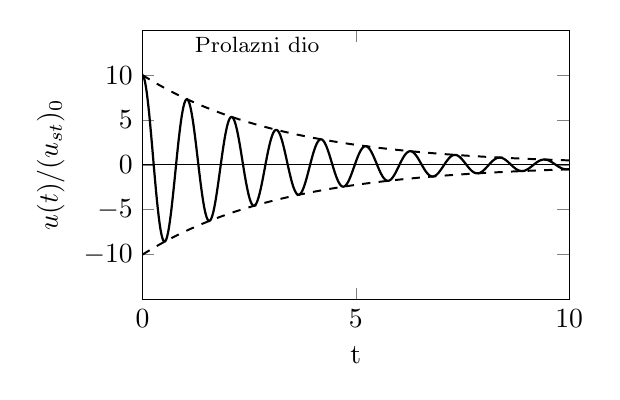
\begin{tikzpicture}
\begin{axis} [
    title={\footnotesize{Prolazni dio}},
    title style={at={(0.1,0.95)}, anchor=north west, draw=none, fill=none},
    height=5cm,
    width=7cm,
    xlabel=t,ylabel=$u(t)/(u_{st})_0$,
    ylabel near ticks, ylabel style={anchor=south},
    xmin = 0, xmax = 10,
    ymin = -15, ymax = 15,
    xtick = {0, 5, 10, 15, 20},
    ytick = {-10, -5, 0, 5, 10},
 ]
    \draw[thin] (0,0) -- (20,0);
    \addplot [
        domain=0:20,
        samples=200,
        color=black,
        dashed,line width=0.25mm,
    ] {10*exp(-0.05*6*x)};
    \addplot [
        domain=0:20,
        samples=200,
        color=black,
        dashed,line width=0.25mm,
    ] {-10*exp(-0.05*6*x)};
    \addplot [
        domain=0:20,
        samples=1000,
        color=black,
        thick,
    ] {10*exp(-0.05*6*x)*cos(6*deg(x))};
\end{axis}
\end{tikzpicture}
\end{subfigure}
\hfill
%
%
%
\begin{subfigure}[b][][r]{0.05\textwidth}
    \centering
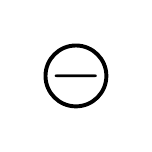
\begin{tikzpicture}[scale=5]
    \draw[thick, line width=0.5mm] (0,0) circle (2.2pt);
    \node[circle,fill=none,color=black] at (0,0) {\textbf{\Huge{$-$}}};
\end{tikzpicture}
\end{subfigure}
\hfill
%
%
%
\begin{subfigure}[c][][r]{0.45\textwidth}
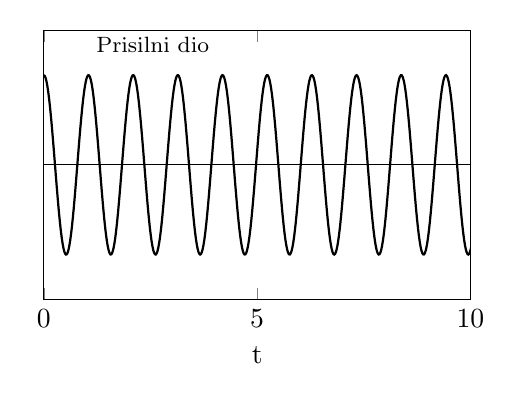
\begin{tikzpicture}
\begin{axis} [
    title={\footnotesize{Prisilni dio}},
    title style={at={(0.1,0.95)}, anchor=north west, draw=none, fill=none},
    height=5cm,
    width=7cm,
    xlabel=t,%ylabel=$u(t)/(u_{st})_0$,
%    ylabel near ticks, ylabel style={anchor=south},
    xmin = 0, xmax = 10,
    ymin = -15, ymax = 15,
    xtick = {0, 5, 10, 15, 20},
%    ytick = {-10, -5, 0, 5, 10},
    ytick=\empty,
 ]
    \draw[thin] (0,0) -- (20,0);
    \addplot [
        domain=0:20,
        samples=1000,
        color=black,
        thick,
    ] {10*cos(6*deg(x))};
\end{axis}
\end{tikzpicture}
\end{subfigure}
\vfill
%
%
%
\begin{subfigure}[b][3pt][c]{1\textwidth}
    \centering
    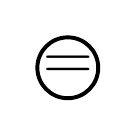
\begin{tikzpicture}[scale=5]
        \draw[thick, line width=0.5mm] (0,0) circle (2.2pt); 
        \node[circle,fill=none,color=black] at (0,0) {\textbf{\Huge{$=$}}};
    \end{tikzpicture}
\end{subfigure}
\vfill
%
%
%
\begin{subfigure}[t][][c]{1\textwidth}
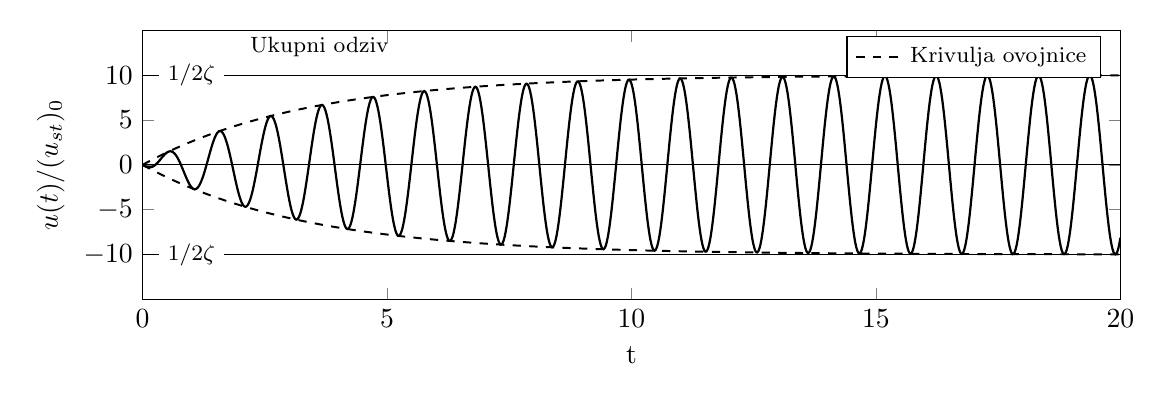
\begin{tikzpicture}
\begin{axis} [
    title={\footnotesize{Ukupni odziv}},
    title style={at={(0.1,0.95)}, anchor=north west, draw=none, fill=none},
    height=5cm,
    width=14cm,
    xlabel=t,ylabel=$u(t)/(u_{st})_0$,
    ylabel near ticks, ylabel style={anchor=south},
    xmin = 0, xmax = 20,
    ymin = -15, ymax = 15,
    xtick = {0, 5, 10, 15, 20},
    ytick = {-10, -5, 0, 5, 10},
 ]
    \draw[thin] (0,0) -- (20,0);

    \addplot [
        domain=0:20,
        samples=200,
        color=black,
        dashed,line width=0.25mm,
    ] {10*(exp(-0.05*6*x)-1)};

    \addplot [
        domain=0:20,
        samples=200,
        color=black,
        dashed,line width=0.25mm,
    ] {-10*(exp(-0.05*6*x)-1)};

    \addlegendentry{\footnotesize{Krivulja ovojnice}}

    \addplot [
        domain=0:20,
        samples=1000,
        color=black,
        thick,
    ] {10*exp(-0.05*6*x)*cos(6*deg(x))-10*cos(6*deg(x))};
%    \addlegendentry{\footnotesize{Ukupni odziv}}


    
    \draw[thin] (0,10) -- (20,10);
    \node[rectangle, fill=white] at (1,10) {\footnotesize{$1/2\zeta$}};
    \draw[thin] (0,-10) -- (20, -10);
    \node[rectangle, fill=white] at (1,-10) {\footnotesize{$1/2\zeta$}};

    \end{axis}
\end{tikzpicture}
\end{subfigure}

 
    \caption{Odziv prigušenog sustava na pobudu rezonantnom frekvencijom}
    \label{fig:rezonanca-priguseno}
\end{figure}

O prigušenju u rezonanci ovise slijedeći parametari odziva:
\begin{itemize}
    \item brzina dostizanje ustaljenog stanja (maksimalne amplitude) - brzina dostizanja 
        ustaljenog stanja raste proporcionalno s prigušenjem (veće prigušenje $\to$ strmija krivulja
        ovojnice $\to$ brže dostizanje ustaljenog stanja).

    \item vrijednost maksimalne amplitude - obrnuto proporcionalna od vrijednosti
        prigušenja, definirana izrazom \eqref{eq:rezonanca_amplituda}. 
        (veće prigušenje, manja maksimalna amplituda, vidljivo i u frekvencijskim funkcijama odziva)
\end{itemize}

Određivanje broja titraja koji je potreban za dostizanje ustaljenog stanja vrši
se pomoću funkcije koja opisuje krivulju ovojnice. Pretpostavka je da ekstrem
nastupa nakon $j$ titraja ($j$ je prirodni broj), a vrijeme nastupa minimuma je
$t=2\pi j/\omega$. 
\begin{equation}\label{eq:prirastEkstremaPriguseno}
    u\left(\frac{2\pi j}{\omega_n}\right) \approx
        u_0(e^{-\zeta\omega_n\frac{2\pi j}{\omega_n}}-1)\cos\left(\omega_n\frac{2\pi
        j}{\omega_n}\right)
\end{equation}
Gdje je:
\begin{table}[H]
    \begin{tabular}{c c}
        $j$ & redni broj titraja\\
        $u_0=(u_{st})_0/2\zeta$ & maksimalna amplituda\\
    \end{tabular}
\end{table}
Kako se radi o ekstremnoj vrijednosti, funkcija kosinus iznosi $\pm 1$ pa jednadžba
pod \eqref{eq:prirastEkstremaPriguseno} glasi:
\begin{equation}\label{eq:MiniMaxPriguseno}
     u\left(\frac{2\pi j}{\omega_n}\right) = u_j = 
        \pm u_0(e^{-2\pi\zeta j}-1)
\end{equation}

Za maksimume jednadžba pod \eqref{eq:MiniMaxPriguseno} postaje
\begin{equation}
    |u_j| = -u_0(e^{-2\pi\zeta j} -1) = u_0(1-e^{-2\pi\zeta j})
\end{equation}

Za relativne vrijednosti\footnote{Postotci od maksimalne amplitude}:
\begin{equation}
    u[j] = \frac{|u_j|}{u_0}=1-e^{-2j\zeta\pi}
\end{equation}
Izraz ima smisla samo za diskretne vrijednosti argumenta $j$, odnosno za $j \in
\mathbb{N}$.

\par
\begin{minipage}[b][][l]{0.1\textwidth}
\begin{table}[H]
    \begin{tabular}{c | c}
       \hline
        $\zeta$ & $j$\\
        \hline
        $0.01$ & $48$\\
        \hline
        $0.02$ & $24$\\
        \hline
        $0.05$ & $10$\\
        \hline
        $0.1$ & $5$\\
        \hline
        $0.2$ & $3$\\
        \hline
    \end{tabular}
    \caption{Očitanje s grafa}
    \label{table:prirast-rezonanca-priguseno}
\end{table}
\end{minipage}
\hfill
\begin{minipage}[b][][r]{0.8\textwidth}
\begin{figure}[H]
    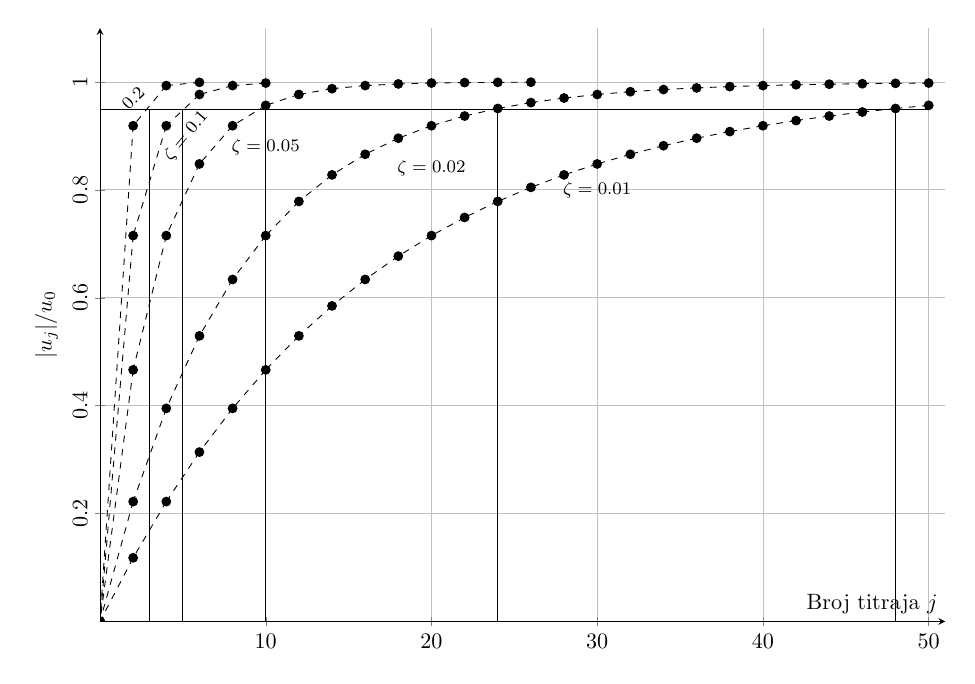
\begin{tikzpicture}[scale=0.8]
    \begin{axis} [
        height=11cm,
        axis lines=center,
        xlabel=Broj titraja $j$,
        ylabel={$|u_j|/u_0$},
        ylabel near ticks, ylabel style={anchor=south},
        xmin=0, xmax=51,
        ymin=0, ymax=1.1,
        xtick={0,10,20,30,40,50},
        ytick={0.2,0.4,0.6,0.8,1}, yticklabel style={rotate=90},
        grid=both,
    ]

        %zeta = 0.2
        \pgfplotsinvokeforeach{0, 2, 4, 6}
        {
            \filldraw( #1,{1 - exp(-2*pi*0.2*#1}) circle[radius=2pt, fill=black];
            \draw[dashed]( #1,{1 - exp(-2*pi*0.2*#1}) -- ( {#1-2}, {1-exp(-2*pi*0.2*(#1-2)});
        }

        %zeta = 0.1
        \pgfplotsinvokeforeach{0, 2, 4, ..., 10}
        {
            \filldraw( #1,{1 - exp(-2*pi*0.1*#1}) circle[radius=2pt, fill=black];
            \draw[dashed]( #1,{1 - exp(-2*pi*0.1*#1}) -- ( {#1-2}, {1-exp(-2*pi*0.1*(#1-2)});
        }

        %zeta = 0.05
        \pgfplotsinvokeforeach{0, 2, 4, ..., 26}
        {
            \filldraw( #1,{1 - exp(-2*pi*0.05*#1}) circle[radius=2pt, fill=black];
            \draw[dashed]( #1,{1 - exp(-2*pi*0.05*#1}) -- ( {#1-2}, {1-exp(-2*pi*0.05*(#1-2)});
        }

        %zeta = 0.02
        \pgfplotsinvokeforeach{0, 2, 4, ..., 50}
        {
            \filldraw( #1,{1 - exp(-2*pi*0.02*#1}) circle[radius=2pt, fill=black];
            \draw[dashed]( #1,{1 - exp(-2*pi*0.02*#1}) -- ( {#1-2}, {1-exp(-2*pi*0.02*(#1-2)});
        }

        %zeta = 0.01
        \pgfplotsinvokeforeach{0, 2, 4, ..., 50}
        {
            \filldraw( #1,{1 - exp(-2*pi*0.01*#1}) circle[radius=2pt, fill=black];
            \draw[dashed]( #1,{1 - exp(-2*pi*0.01*#1}) -- ( {#1-2}, {1-exp(-2*pi*0.01*(#1-2)});
        }

        %oznake
        \node at (30,0.80) {\footnotesize{$\zeta=0.01$}};
        \node at (20,0.84) {\footnotesize{$\zeta=0.02$}};
        \node at (10,0.88) {\footnotesize{$\zeta=0.05$}};
        \node[rotate=50] at (5.2, 0.9) {\footnotesize{$\zeta=0.1$}};
        \node[rotate=45] at (2, 0.97) {\footnotesize{$0.2$}};

        %ocitanja
        \draw[thin] (0,0.95) -- (50,0.95);
        %za 0.01
        \draw[thin] (48,0) -- (48,0.95);
        %za 0.02
        \draw[thin] (24,0) -- (24,0.95);
        %za 0.05
        \draw[thin] (10,0) -- (10,0.95);
        %za 0.1
        \draw[thin] (5,0) -- (5,0.95);
        %za 0.2
        \draw[thin] (3,0) -- (3,0.95);
    \end{axis}
\end{tikzpicture}

    \label{fig:prirast-rezonanca-priguseno}
    \caption{Ovisnost amplitude odziva o broju titraja u rezonanci}
\end{figure}
\end{minipage}
\vspace{6pt}

Uočimo da je uz slabije prigušenje potrebno više titraja za dostizanje ustaljenog
stanja odnosno maksimalne amplitude. Očitanja vrijednosti sa grafa prikazana su u
\ref{table:prirast-rezonanca-priguseno}.



    \newpage
    \subsection{Rezonanca sustava bez prigušenja}
Za sustav bez prigušenja, rezonantne frekvencije za $R_d$, $R_v$ i $R_a$ jednake su
prirodnoj frekvenciji sustava što se dobije uvrštavanjem $\zeta = 0$ u \eqref{eq:rd_rezonanca} i 
\eqref{eq:ra_rezonanca}. 
\par

Primjetimo da je maksimalni dinamički koeficijent $R_d$ (za $\omega/\omega_n = 1$) 
neograničen, tj $R_d\to \infty$ što se vidi i u jednadžbi \eqref{eq:fazniSpektarNepriguseno} 
te na grafu \ref{fig:frf-nepriguseno}. U slijedećoj jednadžbi prikazana je vremenska 
funkcija pomaka sustava za homogene početne uvjete:
\begin{equation}
    u(t)=\frac{p_0}{k}\frac{1}{1-(\omega/\omega_n)}
            \left(\sin(\omega t) - \frac{\omega}{\omega_n}\sin(\omega_n t)\right)
\end{equation}

Uočimo da za $\omega = \omega_n$ navedena jednadžba više ne vrijedi (djeljenje s
nulom). Novu jednadžbu možemo odrediti na slijedeći način:
\begin{equation}\label{eq:limes}
    \lim_{\omega\to\omega_n}{u(t)} = 
        \frac{p}{k}\frac{1}{1-(\omega/\omega_n)^2}
            \left(\sin(\omega t) - \frac{\omega}{\omega_n}\sin(\omega_n t)\right)
\end{equation}

Navedeni limes je oblika $\frac{0}{0}$, pa ga je moguće rješiti L'Hopitalovim
pravilom. Deriviranjem funkcije po $\omega$ dobijemo:
\begin{equation}\label{eq:lhopitalovo_limes}
    \lim_{\omega\to\omega_n}\frac{d}{d\omega}u(t)=
    \lim_{\omega\to\omega_n} \left[
        \frac{p_0}{k}\frac{1}{-2(\omega/\omega_n)}
            \left(t\cos(\omega t) - \frac{1}{\omega}\sin(\omega_n t)\right)
           \right]
\end{equation}
Uvrštavanjem $\omega=\omega_n$ dobijemo:
\begin{equation}\label{eq:odziv_rezonanca}
    u(t)=-\frac{1}{2}\frac{p_0}{k}(\omega_n\cos(\omega_n t)-\sin(\omega_nt))
\end{equation}

Iz navedene jednadžbe vidljivo je da usprkos neograničenom dinamičkom faktoru
neizmjerno velika amplituda ne nastupa trenutno, već dolazi do njezinog 
postupnog rasta. Djeljenjem izraza \eqref{eq:odziv_rezonanca} statičkim pomakom i
uvrštavanjem $\omega_n=\frac{2\pi}{T_n}$ dobijemo:
\begin{equation}\label{eq:rezonanca_period}
    \frac{u(t)}{(u_{st})_0}=-\frac{1}{2}
        \left(\frac{2\pi t}{T_n}
                \cos\left(\frac{2\pi t}{T_n}\right)
                -
                \sin\left(\frac{2\pi t}{T_n}\right)
        \right)
\end{equation}
Gdje je:
\begin{table}[H]
    \begin{tabular} {r l}
        $T_n$ & period titranja\\
    \end{tabular}
\end{table}

Iz prethodne jednadžbe slijedi da ekstremi nastupaju svaki poluperiod ($T_n/2$), pri
čemu prvo nastupa maksimum a zatim minimum. Vrijeme nastupa ekstrema za određeni
redni broj titraja prikazuju slijedeće jednadžbe:
\begin{itemize}
    \item za maksimum: $t=(i-\frac{1}{2})T_n$
    \item za minimum: $t=jT_n$
\end{itemize}
Gdje je:
\begin{table}[H]
    \begin{tabular} {r l}
        $t$ & vrijeme nastupa ekstrema\\
        $i$ & redni broj titraja\\
    \end{tabular}
\end{table}
Iznos ekstrema određujemo uvrštavanjem vremena nastupa ekstrema u jednadžbu
\eqref{eq:rezonanca_period} te slijedi:
\begin{enumerate}
    \item iznos maksimuma za j-ti titraj: $u_j=(u_{st})_0\pi(j-\frac{1}{2})$
    \item iznos minimuma za j-ti titraj: $u_j=-(u_{st})_0\pi\cdot j$ 
\end{enumerate}

Prirast maksimuma određujemo razlikom između iznosa maksimuma trenutnog i slijedećeg
titraja što prikazuje slijedeća jednadžba:
\begin{equation}\label{eq:prirast_maksimuma}
    \begin{split}
        |u_{j+1}|-|u_j| &=(u_{st})_0\pi((j+1)-\frac{1}{2})-(u_{st})_0\pi(j-\frac{1}{2})\\
        |u_{j+1}|-|u_j| &= \frac{p_0}{k}\pi
    \end{split}
\end{equation}

Analogno tome određuje se i prirast minimuma koji glasi:
\begin{equation}\label{eq:prirast_minimuma}
    \begin{split}
        u_{j+1}-u_j &= -(u_{st})_0\pi(j+1)-(-(u_{st})_0\pi j)\\
        u_{j+1}-u_j &= -\frac{p_0}{k}\pi
    \end{split}
\end{equation}

Uočimo da su prirasti ekstrema linearni, stoga krivulju ovojnice čine pravaci čiji
su koeficjenti smjera prikazani u nastavku:
\begin{equation}\label{eq:koef_smjera_envelopa}
    k_{1,2}=\pm\frac{1}{2}\frac{p_0}{k}\omega_n
\end{equation}

\begin{figure}[H]
    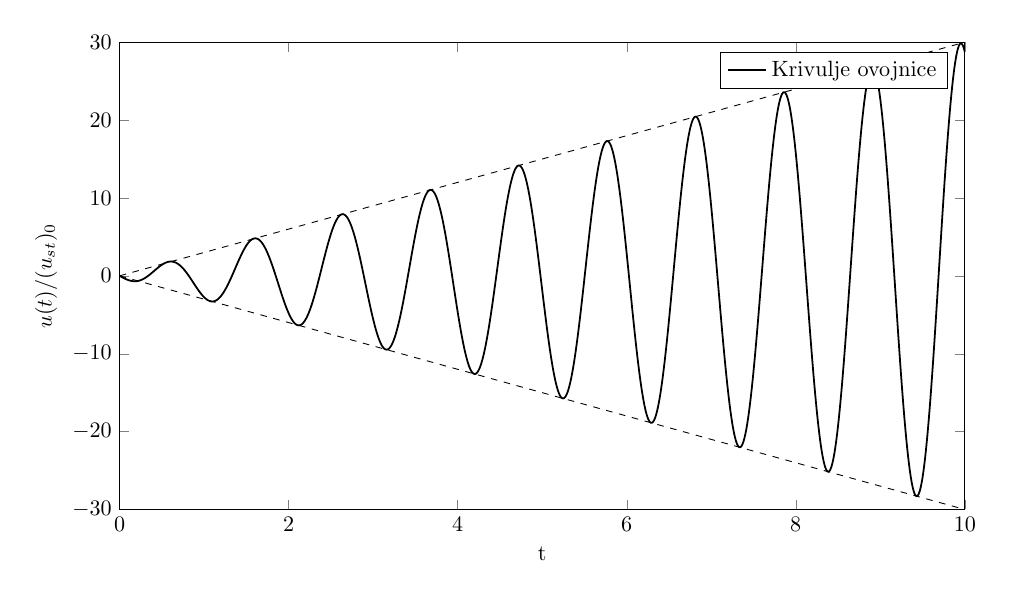
\begin{tikzpicture}[scale=0.8]
    \begin{axis} [
        height=9cm,
%        axis lines = center,
        xlabel=t,ylabel=$u(t)/(u_{st})_0$,
        ylabel near ticks, ylabel style={anchor=south},
        xmin = 0, xmax = 10,
        ymin = -30, ymax =30,
        xtick = {0, 2, 4, 6, 8, 10},
        ytick = {-30,-20,-10,0,10,20,30},
     ]
        \addplot [
            domain=0:10,
            samples=1000,
            color=black,
            thick,
        ] {-0.5*(6*x*cos(6*deg(x))+sin(6*deg(x))};

        \addplot [
            domain=0:10,
            samples=100,
            color=black,
            dashed,
        ] {0.5*6*x};

        \addplot [
            domain=0:10,
            samples=100,
            color=black,
            dashed,
        ] {-0.5*6*x};
        \addlegendentry{Krivulje ovojnice}
    \end{axis}
\end{tikzpicture}

    \label{rezonanca-nepriguseno}
    \caption{Rezonanca neprigusenog sustava}
\end{figure}



    \newpage
    \subsection{Analiza područja rezonance}
Osim rezonantne frekvencije potrebno je odrediti i pojas polovice snage vrha
frekvencijske funkcije odziva, koji je prikazan na slici \ref{fig:hpb}. Pojas polovice
snage vrha frekvencijske funkcije odziva bitan je iz dva razloga:
\begin{enumerate}
    \item osim pobude rezonantnom frekvencijom, opasne su i pobude frekvencijama iz
        njezinog okoliša. Navedeni okoliš definiran je pojasom polovice snage.
    \item Zbog praktične primjene - pojas polovice snage koristi se u pokusima
        za određivanje stupnja prigušenja konstrukcija
\end{enumerate}
\begin{figure}[H]
    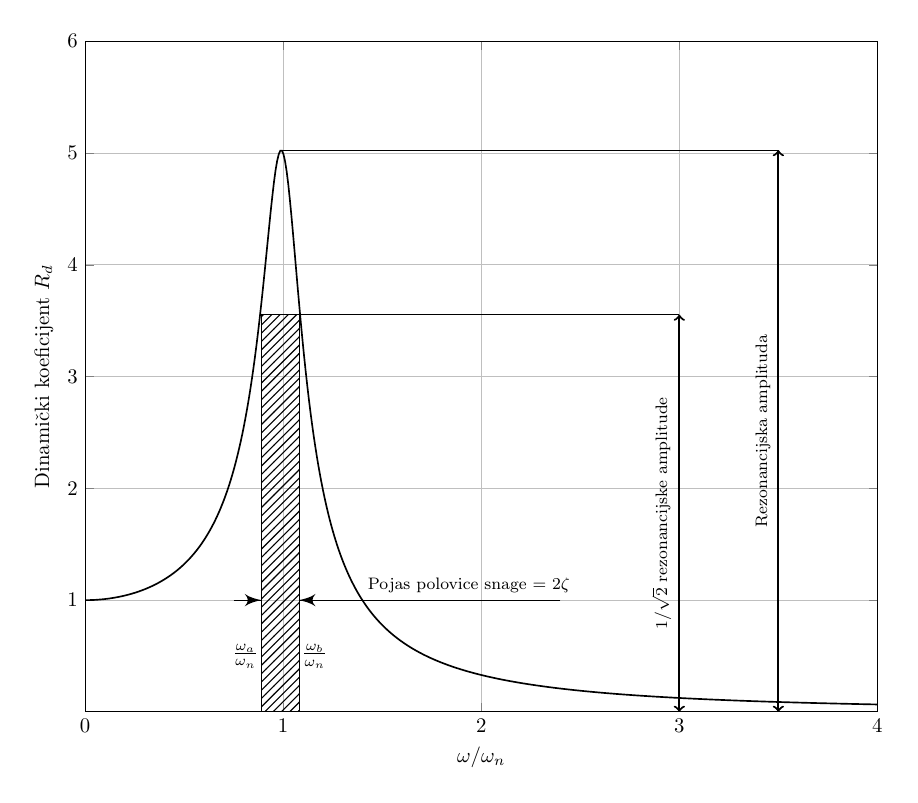
\begin{tikzpicture}[scale=0.75]
    \begin{axis} [
        ylabel = Dinamički koeficijent $R_d$,
        xlabel = $\omega/\omega_n$,
        xmin = 0, xmax = 4,
        ymin = 0, ymax = 6,
        xtick = {0, 1, 2, 3, 4},
        ytick = {1, 2, 3, 4, 5, 6},
        grid=both, %minor tick num=0.5,
     ]

    \addplot [
        domain=0:4,
        samples=500,
        color=black,
        thick,
    ]{1/((1-x^2)^2+(2*0.1*x)^2)^0.5};

    \draw[color=black,pattern=north east lines, pattern color=black] (0.89,0) 
        rectangle (1.08,3.555);
    \draw[strelica1] (0.75, 1) -- (0.89, 1);
    \draw[strelica1] (2.4, 1) -- (1.08,1)
        node[above,pos=0.35] {\footnotesize{Pojas polovice snage = $2\zeta$}};

    %kotiraj rezonancijsku amplitudu
    \draw[<->,line width=1pt] (3.5,0) -- (3.5, 5.027)
        node[pos=0.5,above,rotate=90]{\footnotesize{Rezonancijska amplituda}};
    \draw(0.995,5.027) -- (3.5,5.027);

    \node at (0.81, 0.5) {$\frac{\omega_a}{\omega_n}$};
    \node at (1.16, 0.5) {$\frac{\omega_b}{\omega_n}$};

    %kotiraj pojas polovice snage
    \draw[<->,line width=1pt] (3,0) -- (3,3.555)
        node[pos=0.5,above,rotate=90]{\footnotesize{$1/\sqrt{2}$ rezonancijske amplitude}};
    \draw(1,3.555) -- (3,3.555);

    \end{axis}
\end{tikzpicture}

    \caption{Definicija pojasa polovice snage}
    \label{fig:hpb}
\end{figure}
Dinamički faktor pomaka $R_d$ za odziv dvostruko manje snage od odziva maksimalnog
dinamičkog faktora računa se prema slijedećoj relaciji:
\begin{equation}\label{eq:hpb}
    R_d = \frac{1}{\sqrt{2}}R_d^{max}
\end{equation}

Sa slike je vidljivo da je dinamički faktor $R_d$ iz \eqref{eq:hpb} definiran za
dvije vrijednosti frekvencije pobude: $\omega_a$ i $\omega_b$. Raspisivanjem
jednadžbe pod \eqref{eq:hpb} dobijemo:

\begin{equation}\label{eq:hpb_izvod_1}
        \frac{1}{\sqrt{(1-(\omega/\omega_n)^2)^2+(2\zeta\omega/\omega_n)^2}}=
            \frac{1}{\sqrt{2}}\frac{1}{2\zeta\sqrt{1-\zeta^2}}\\
\end{equation}

Kvadriranjem \eqref{eq:hpb_izvod_1} dobijemo:
\begin{equation}\label{eq:hpb_izvod_2}
    \left(1-\left(\frac{\omega}{\omega_n}\right)^2\right)^2
    +\left(2\zeta\frac{\omega}{\omega_n}\right)^2 =
    8\zeta^2(1-\zeta^2)
\end{equation}

Raspisivanjem i grupiranjem po $\omega/\omega_n$ dobijemo:
\begin{equation}\label{eq:hpb_izvod_3}
    \left(\frac{\omega}{\omega_n}\right)^4
    -2(1-2\zeta^2)\left(\frac{\omega}{\omega_n}\right)^2
    +1-8\zeta^2(1-\zeta^2)=0
\end{equation}

Izraz \eqref{eq:hpb_izvod_3} je kvadratna jednadžba, a njezinim rješavanjem (po
$\omega/\omega_n$) dobijemo:
\begin{equation}\label{eq:hpb_kvadratna_1}
    \left(\frac{\omega}{\omega_n}\right)^2 = 
        (1-2\zeta^2)\pm 2\zeta\sqrt{1-\zeta^2}
\end{equation}

Za $\zeta^2 \approx 0$ izraz \eqref{eq:hpb_kvadratna_1} postaje:
\begin{equation}
    \left(\frac{\omega}{\omega_n}\right)^2 \approx
        1 \pm 2\zeta
\end{equation}

Odnosno:
\begin{equation}\label{eq:hpb_kvadratna_2}
    \left(\frac{\omega}{\omega_n}\right)\approx
        \sqrt{1 \pm 2\zeta}
\end{equation}
Jednadžba \eqref{hpb_kvadratna_2}, nakon aproksimacije korijena s prva dva člana Taylorovog
reda glasi:
\begin{equation}\label{eq:hpb_kvadratna_konacno}
    \frac{\omega}{\omega_n} = 1 \pm \zeta
\end{equation}

Frekvencije $\omega_a$ i $\omega_b$ dobiju se iz \eqref{eq:hpb_kvadratna_konacno}:
\begin{align}
    \omega_a &= (1-\zeta)\omega_n\\
    \omega_b &= (1+\zeta)\omega_n\\
\end{align}

Oduzimanjem $\omega_b-\omega_a$ dobijemo:
\begin{equation}\label{eq:hpb_zeta_omega}
        2\zeta = \frac{\omega_b-\omega_a}{\omega_n}
\end{equation}

Te konačno, dijeljenjem brojnika i nazivnika s $2\pi$:
\begin{equation}\label{eq:hpb_zeta_f}
    \zeta\approx\frac{f_b-f_a}{2f_n}
\end{equation}

Gdje je $f=\omega/2\pi$ kružna frekvencija. Jednadžbe pod \eqref{eq:hpb_zeta_omega}
i \eqref{eq:hpb_zeta_f} bitne su jer omogućuju određivanje koeficijenta relativnog prigušenja
$\zeta$ bez potrebe za poznavanjem intenziteta sile pobude. 



    \newpage
    \subsection{Praktična primjena matematičkog modela}
Definiranjem matematičkog modela prigušenog sustava s jednim stupnjem slobode,
pobuđenog sinusnom silom postavljeni su temelji za eksperimentalno određivanje
stupnja prigušenja i prirodne frekvencije. Stupnanj prigušenja jest veličina od
izuzetne praktične važnosti, a nije ga moguće odrediti teoretski iz projektnih
parametara, već se mora odrediti eksperimentalno. %Isto tako izmjerena vrijednost prirodne
%frekvencije jest stvarno svojstvo konstrukcije, s kojim se uspoređuje teoretski
%određena prirodna frekvencija. 
Ispitivanje koje će biti razmatrano u ovome radu naziva se \textit{rezonancijski
pokus}.

%Matematički model prigušenog sustava s jednim stupnjem slobode, pobuđen sinusnom
%silom koristi se priklikom određivanja stupnja prigušenja i prirodne frekvencije 
%realnih konstrukcija. Stupanj prigušenja je veličina od izuzetne važnosti koju nije
%moguće odrediti analitički, nego ju je potrebno odrediti ispitivanjima. 

Ispitivanja se provode \textit{vibracijskim uređajem}. Vibracijski uređaj se sastoji
od dvije košare sa utezima na uspravnoj osovini koje rotiraju u suprotnim smjerovima
konstantnom kutnom brzinom $\omega$. Osovina je pričvršćena za metalnu ploču koja se
kruto povezuje s građevinom. 

\begin{figure}[H]
        \begin{subfigure}[b][][l]{0.45\textwidth}
        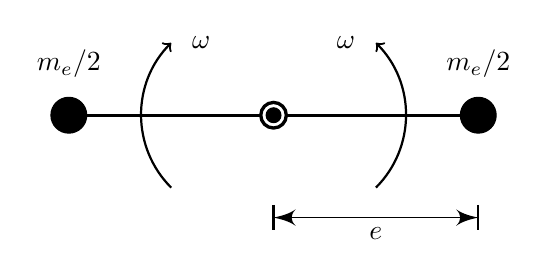
\begin{tikzpicture}[scale=0.65][>=latex']

    %lezaj
    \draw[very thick] (0,0) circle (0.25);
    \filldraw[fill=black] (0,0) circle (0.145);

    %stapovi
    \draw[very thick] (0.25,0) -- (4,0);
    \draw[very thick] (-0.25,0)--(-4,0);

    %utezi
    \filldraw[fill=black] (4,0) circle (0.35);
    \filldraw[fill=black] (-4,0)circle (0.35);

    %oznake
    \draw[strelica1](0,-2) -- (4,-2)
        node[pos=0.5,below] {\textbf{{$e$}}};
    \draw[strelica1](4,-2) -- (0,-2);

    \draw[thick] (0,-1.75) -- (0,-2.25);
    \draw[thick] (4,-1.75) -- (4,-2.25);

    \draw[->,thick] (2,-1.414) arc [start angle=-45, end angle=45, radius=2];

    %namjesti lijevu strelicu (za ovo mora postojat laksi nacin ali ne da mi se istrazivat trenutno)
    \draw[<-,thick,shift={(-2,1.414)},rotate=180] (0,0)arc [start angle=-45, end angle=45, radius=2];
    \node at (1.414,1.414) {\textbf{{$\omega$}}};
    \node at (-1.414,1.414) {\textbf{{$\omega$}}};

    %za mase
    \node at (4,1) {\textbf{{$m_e/2$}}};
    \node at (-4,1) {\textbf{{$m_e/2$}}};
\end{tikzpicture}


        \caption{}
        \label{fig:vibracijski-t0}
    \end{subfigure}
    \hfill
    \begin{subfigure}[b][][r]{0.45\textwidth}
        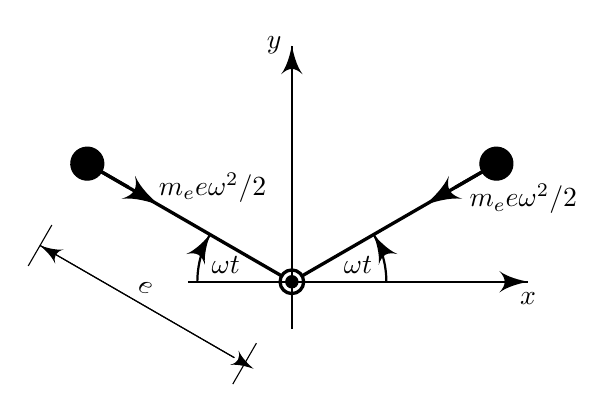
\begin{tikzpicture}[scale=0.6,>=latex']

    %koordinatni sustav
    \draw[thick,strelica1] (-2.2,0) -- (5,0)
        node[pos=1,below]{{$x$}};
    \draw[thick,strelica1] (0,-1) -- (0,5)
        node[pos=1,left]{{$y$}};

    %lezaj
    \draw[very thick] (0,0) circle (0.25);
    \filldraw[fill=black] (0,0) circle (0.130);

    %stapovi
    \draw[very thick, rotate=-30] (-0.25,0) -- (-5,0);
    \draw[very thick, rotate=30]  (0.25,0) -- (5,0);

    %mase
    \filldraw[fill=black,rotate=30] (5,0) circle (0.35);
    \filldraw[fill=black,rotate=-30] (-5,0)circle (0.35);

    %oznake
    \draw[strelica1,shift={(-1,-1.732)},rotate=60] (0,0.25) -- (0,5)
        node[pos=0.5, above,rotate=-30]{{$e$}};
    \draw[strelica0,shift={(-1,-1.732)},rotate=60] (0,0.25) -- (0,5);

    \draw[shift={(-1,-1.732)},rotate=-30] (0,-0.5) -- (0,0.5);
    \draw[shift={(-1,-1.732)},shift={(-4.33,2.5)},rotate=-30] (0,-0.5) -- (0,0.5);

    %kut
    \draw[thick, strelica1] (2,0) arc[start angle=0, end angle=30, radius=2];
    \draw[thick, strelica1, shift={(-2,0)}, rotate=180] (0,0) arc[start angle=0, end angle=-30, radius=2];
    \node at (1.4,0.35) {{$\omega t$}};
    \node at (-1.4,0.35){{$\omega t$}};

    %sile
    \draw[strelica0,very thick,shift={(-3.46,2)},rotate=60] (0,0)--(0,1)
        node[pos=0,right=2.5mm] {{$m_ee\omega^2/2$}};

    \draw[strelica0,very thick,shift={(4.33,2.5)},rotate=30] (-1,0)--(0,0)
        node[pos=-0.5,right=3mm] {{$m_ee\omega^2/2$}};
\end{tikzpicture}


        \caption{}
        \label{fig:vibracijski-t}
    \end{subfigure}
    \caption{Shematski prikaz vibracijskog uređaja: 
            (\subref{fig:vibracijski-t0}) u inicijalnom položaju;
            (\subref{fig:vibracijski-t}) položaj nakon vremena t}
    \label{fig:vibracijski}
\end{figure}

Sila pobude građevine jest ukupna centrifugalna sila vibracijskog uređaja, koja je 
jednaka je sumi centrifugalnih sila pojedinih masa.
Horizontalne komponente su jednakog intenziteta ali suprotnog smjera pa se
poništavaju, stoga sila pobude je jednaka sumi vertikalnih komponenti, odnosno:
\begin{equation}
    p(t)=(m_ee\omega^2)\sin(\omega t)
\end{equation}

Odziv sustava s jednim stupnjem slobode na pobudu vibracijskim uređajem opisan je
slijedećom diferencijalnom jednadžbom:
\begin{equation}
    m\ddot{u}+c\dot{u}+ku=(m_ee\omega^2)\sin(\omega t)
\end{equation}

Amplituda prisilnog pomaka glasi (iz \eqref{eq:prisilni_alternativno_rjesenje_Rd}):
\begin{equation}
    u_0=\frac{m_ee}{k}\omega^2R_d = \frac{m_ee}{m}\left(\frac{\omega}{\omega_n}\right)^2R_d
\end{equation}

Amplituda prisilnog ubrzanja (iz \eqref{eq:R_a}
\begin{equation}
    \ddot{u}_0=\frac{m_ee}{m}\omega^2R_a=\frac{m_ee\omega_n^2}{m}\left(\frac{\omega}{\omega_n}\right)^2R_a
\end{equation}

\begin{figure}[H]
    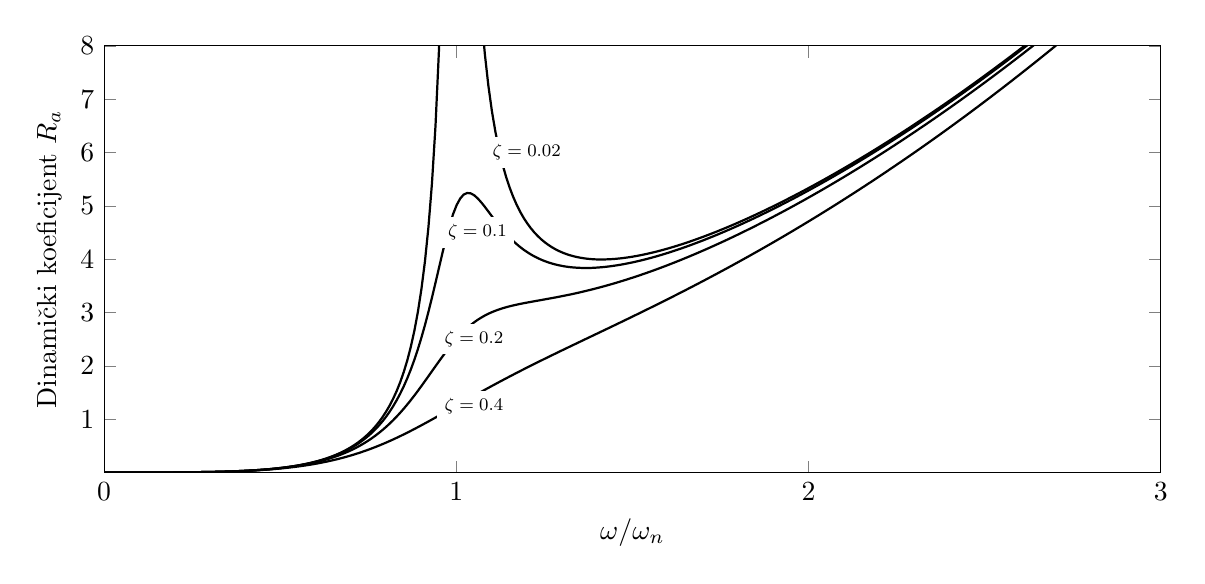
\begin{tikzpicture}
    \begin{axis} [
        height=7cm,
        ylabel = Dinamički koeficijent $R_a$,
        xlabel = $\omega/\omega_n$,
        xmin = 0, xmax = 3,
        ymin = 0, ymax = 8,
        xtick = {0, 1, 2, 3},
        ytick = {1, 2, 3, 4, 5, 6, 7, 8},
     ]

    \foreach \i in {0.4, 0.2, 0.1, 0.02}
        {
            \addplot [
                domain=0:10,
                samples=1000,
                color=black,
                thick,
            ]{x^4/((1-x^2)^2+(2*\i*x)^2)^0.5};
        }
   \pgfplotsinvokeforeach{0.4,0.2}
        {
            \node[rectangle,fill=white,scale=0.8] at 
                (1.05,{1/(2*#1)}) {\footnotesize{$\zeta=#1$}};
        }
    \node[rectangle,fill=white,scale=0.8] at 
        (1.06,4.5) {\footnotesize{$\zeta=0.1$}};

    \node[rectangle,fill=white,scale=0.8] at 
        (1.2,6) {\footnotesize{$\zeta=0.02$}};
    \end{axis}

\end{tikzpicture}

    \caption{Amplituda ubrzanja u ovisnosti o omjeru frekvencija}
    \label{fig:ra-vibracijski}
\end{figure}

Na grafu sa slike \ref{fig:ra-vibracijski} vidljivo je da daljnjim porastom frekvencije pobude (iznad prirodne
frekvencije) amplituda prisilnog ubrzanja raste. Navedeni rast se događa jer je
amplituda pobude proporcionalna s $\omega^2$. 
\par

Za određivanje stupnja prigušenja i prirodne frekvencije vrši se
\textit{rezonancijski pokus}, a temelji se na slijedećoj relaciji (iz \eqref{eq:frf_rezonanca})
\begin{equation}\label{eq:rezonancijski_pokus}
    \zeta = \frac{1}{2}\frac{(u_{st})_0}{(u_0)_{\omega=\omega_n}}
\end{equation}
Potrebno je eksperimentalno odrediti amplitudu statičkog pomaka i prirodnu frekvenciju. 
%U eksperimentima se redovito mjeri amplituda ubrzanja a amplitudu pomaka možemo
%dobiti slijedećom relacijom:
%\begin{equation}
%    u_0=\frac{\ddot{u}_0}{\omega^2}
%\end{equation}

Prirodna frekvencija se određuje na slijedeći način:
\begin{enumerate}
    \item pobuđivanje konstrukcije vibracijskim uređajem namještenim na
        određenu frekvenciju $\omega$.
    \item očitavanje faznog kuta. Ako je fazni kut $\phi = 90\degree$, tada je
        prirodna frekvencija $\omega_n$ jednaka frekvenciji pobude $\omega$.
    \item nakon što isčezne prolazni dio odziva, očitava se amplituda prisilnog ubrzanja
\end{enumerate}

Amplitudu prisilnog pomaka možemo dobiti iz amplitude prisilnog ubrzanja korištenjem
slijedeće formule:
\begin{equation}
    u_0=\frac{(\ddot{u}_0)_{\omega=\omega_n}}{(\omega^2)_{\omega=\omega_n}} \quad
    \text{ jer je } \quad
    \ddot{u}(t) = -u_0\omega\sin(\omega t -\phi), \quad
\end{equation}

Da bi bilo moguće odrediti prigušenje sustava prema formuli \eqref{eq:rezonancijski_pokus} 
potrebno je odrediti amplitudu statičkog pomaka $(u_{st})_0=p_{0,max}/k$, gdje je
$p_{0,max}$ amplituda pobude u rezonanci. Amplituda statičkog pomaka se
\textbf{mora} odrediti pokusom, a ne izračunati prema relaciji $p_0/k$ zato što $k$
nije eksperimentalno određen.Vibracijskim uređajem je vrlo teško (ili
nemoguće) prouzročiti veliku \textbf{statičku} silu pobude. Dva su pristupa rješavanju
navedenog problema:
\begin{enumerate}
    \item Sporim rotiranjem velikih masa - Nije najbolje rješenje jer je sila pobude
        proporcionalna s kvadratom kutne brzine rotacije utega. Stoga i za velike mase 
        utega amplituda sile pobude je relativno mala.
    \item Povlačenjem konstrukcije užetom silom koja je jednaka amplitudi sile
        pobude vibracijskim uređajem $p_{0,max}$.
\end{enumerate}

Osim rezonancijskim pokusom, prigušenje i prirodnu frekvenciju moguće je
odrediti \textbf{frekvencijskim krivuljama odziva}. Postupak je slijedeći:
\begin{enumerate}
    \item pobuđivanje konstrukcije vibracijskim uređajem namještenim na određenu
        frekvenciju
    \item određivanje amplitude \textbf{prisilnog} dijela 
    \item namještanje vibracijskog uređaja na drugu frekvenciju, te ponavljanje
        postupka%\footnote{Frekvencije vibracijskog uređaja nalaze se u širem spektru 
%        frekvencija, koji uključuje rezonantnu frekvenciju i frekvencije iz njezine 
%        okoline (i lijevo i desno).} 
\end{enumerate}

Frekvencijska krivulja odziva iscrtava se iz izmjerenih podataka. Frekvencijske
funkcije odziva mogu prikazivati slijedeće ovisnosti:
\begin{enumerate}
    \item ovisnost amplituda ubrzanja o frekvencijskom omjeru - izravno iz
        izmjerenih podataka. Bitno je za naglasiti da je navedena krivulja
        proporcionalna s $\omega^2$.

    \item ovisnost dinamičkog faktora ubrzanja o frekvencijskom omjeru (konstantna
        amplituda pobude) - dijeljenjem izmjerenih podataka s $\omega^2$ 

    \item ovisnost dinamičkog faktora pomaka o frekvencijskom omjeru (konstantna
        amplituda pobude) - dijeljenjem izmjerenih podataka s $\omega^4$.
\end{enumerate}

Stupanj prigušenja i prirodna frekvencija može se odrediti iz bilo koje od navedenih
krivulja. Prirodna frekvencija jednaka je frekvenciji sile pobude u rezonanci.
Stupanj prigušenja određuje se iz \textit{pojasa polovice snage} jednadžbom
\eqref{eq:hpb_zeta_f}, što znači da je potrebno odrediti amplitudu odziva pri
rezonanci te frekvencije za koje je amplituda odziva jednaka $r_{res}/\sqrt{2}$.
\begin{figure}[H]
    \begin{tikzpicture}[scale=0.75]
    \begin{axis} [
        ylabel = Amplituda odziva,
        xlabel = {Frekvencija pobude $f$ $[Hz]$},
        xmin = 3, xmax = 4,
        ymin = 4, ymax = 14,
        xtick = {3.0, 3.25, 3.5, 3.75, 4.0},
%        grid=both,
     ]
        \draw (3.35, 7)  circle[radius=2pt,fill=none,color=black]; 
        \draw (3.45, 9) circle[radius=2pt,fill=none,color=black];
        \draw (3.49, 10) circle[radius=2pt,fill=none,color=black];
        \draw (3.55,12.2) circle[radius=2pt,fill=none,color=black];
        \draw (3.59,12.8) circle[radius=2pt,fill=none,color=black];
        \draw (3.61,12.7) circle[radius=2pt,fill=none,color=black];
        \draw (3.63,12.2) circle[radius=2pt,fill=none,color=black];
        \draw (3.65,11.4) circle[radius=2pt,fill=none,color=black];
        \draw (3.7,10) circle[radius=2pt,fill=none,color=black];
        \draw (3.8,7.2) circle[radius=2pt,fill=none,color=black];
        
        \draw plot [smooth] coordinates{
            (3.35, 7)
            (3.45, 9) 
            (3.49, 10) 
            (3.55,12.2) 
            (3.59,12.8) 
            (3.61,12.7) 
            (3.63,12.2) 
            (3.65,11.4) 
            (3.7,10) 
            (3.8,7.2) 
        };

        %amplituda rezonance
        \draw[thin] (0, 12.8) -- (3.59, 12.8);
        \draw[thin] (3.59, 0) -- (3.59, 12.8);

        %amplituda pojasa polovice snage
        \draw[thin] (0, 9.05) -- (3.735,9.05);
        \draw[thin] (3.45, 0) -- (3.45, 9.05);
        \draw[thin] (3.73, 0) -- (3.735,9.05);

        %oznake frekvencija
        \node[rectangle,fill=white] at (3.59,6) {$f_n=3,590$};
        \node[rectangle,fill=white] at (3.45,5) {$f_a=3,450$};
        \node[rectangle,fill=white] at (3.735,5) {$f_a=3,735$};

        %oznake amplituda
        \node[rectangle,fill=white] at (3.2,12.8) {$12.80$};
        \node[rectangle,fill=white] at (3.2,9.05) {$9.05$};

    \end{axis}
\end{tikzpicture}

    \caption{Frekvencijska funkcija odziva konstruirana pomoću mjerenih podataka}
    \label{fig:frf-poku}
\end{figure}

    \newpage
\chapter{Sustavi s više stupnjeva slobode}
    \section{Jednadžba gibanja slobodnih oscilacija}\label{slobodne_oscilacije}
Jedan od modela sustava s više stupnjeva slobode su $N$ etažni posmični
okviri. Takvi sustavi se sastoje od $N$ koncentriranih masa, što znači da je potrebno 
odrediti $N$ različitih pomaka. Drugim riječima, jednadžba gibanja takvog sustava biti će
zadana kao sustav od N diferencijalnih jednadžbi drugog reda.
\par

Sustav s više stupnjeva slobode, koji će biti razmatran u ovom radu, je dvoetažni
posmični okvir bez prigušenja prikazan na sljedećoj slici, a osnovni pojmovi biti će 
objašnjeni pomoću slobodnih oscilacija navedenog modela.
\begin{figure}[H]
    \begin{subfigure}[b]{0.5\textwidth}
        \centering
        \input{skice/mdf/nepriguseni-sustav-mdf}
        \caption{}
        \label{fig:nepriguseni_sustav_okvir-2dof}
    \end{subfigure}
    \hfill
    \begin{subfigure}[b]{0.5\textwidth}
        \centering
        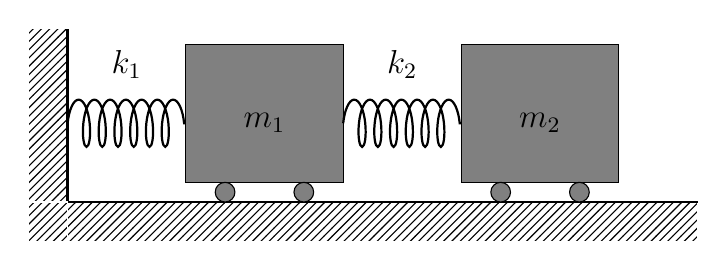
\begin{tikzpicture}
	%podloga
	\draw[white, pattern=north east lines, pattern color=black] (0, 0)
	rectangle (-0.5, 2.2);
	\draw[thick] (0,0) -- (0, 2.2);

	\draw[white, pattern=north east lines, pattern color=black] (0, 0) 
	rectangle (8, -0.5);
	\draw[thick] (0,0) -- (8,0);
	
	\draw[white, pattern=north east lines, pattern color=black] (0, 0)
	rectangle (-0.5, -0.5);

	%uteg
	\filldraw[fill=gray] (1.5, 2) rectangle (3.5, 0.25);
        \filldraw[fill=gray] (5, 2) rectangle (7, 0.25);

	%kotaci
	\filldraw[fill=gray] (2, 0.125) circle (0.125);
	\filldraw[fill=gray] (3, 0.125) circle (0.125);

        \filldraw[fill=gray] (5.5, 0.125) circle (0.125);
        \filldraw[fill=gray] (6.5, 0.125) circle (0.125);

	%opruga
	\draw[thick, decoration={aspect=0.3, segment length=2mm,amplitude=3mm,coil},decorate] (0,1) -- (1.5, 1);
        \draw[thick, decoration={aspect=0.3, segment length=2mm,amplitude=3mm,coil},decorate] (3.5, 1) -- (5, 1);

        \node[draw=none, fill=none] at (0.75, 1.75) {\large{$k_1$}}; 
        \node[draw=none, fill=none] at (2.5,   1) {\large{$m_1$}};

        \node[draw=none, fill=none] at (4.25, 1.75) {\large{$k_2$}};
        \node[draw=none, fill=none] at (6, 1) {\large{$m_2$}};

\end{tikzpicture}

        \caption{}
        \label{fig:nepriguseni_ekvivalentni_sustav-2dof}
    \end{subfigure}
    \vfill
    \vspace{0.5cm}
    \begin{subfigure}[b]{1\textwidth}
        \centering
        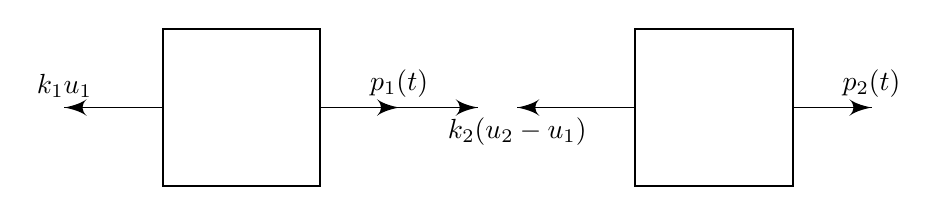
\begin{tikzpicture}
	%uteg_1
	\draw[black,thick] (1.5, 2) rectangle (3.5, 0);

	%sile
	\draw[strelica1] (1.5, 1) -- (0.25, 1) 
		node[pos=1, above]{$k_1u_1$};
	\draw[strelica1] (3.5, 1) -- ( 4.5, 1) 
		node[pos=1, above]{$p_1(t)$};
        \draw[strelica1] (3.5, 1) -- (5.5, 1);
%                node[pos=1, below]{$k_2(u_2-u_1)$};
            
        %uteg_2
        \draw[black,thick] (7.5, 2) rectangle (9.5, 0);

        %sile
        \draw[strelica1] (7.5, 1) -- (6, 1)
                node[pos=1, below]{$k_2(u_2-u_1)$};
        \draw[strelica1] (9.5, 1) -- (10.5, 1)
                node[pos=1, above]{$p_2(t)$};

\end{tikzpicture}

        \caption{}
        \label{fig:sile_nepriguseni_ekvivalentni_sustav-2dof}
    \end{subfigure}
    \caption{Idealizirani sustav s dva stupnja slobode: 
        (\subref{fig:nepriguseni_sustav_okvir-2dof}) dvoetažni posmični okvir;
        (\subref{fig:nepriguseni_ekvivalentni_sustav-2dof}) ekvivalentni model;
        (\subref{fig:sile_nepriguseni_ekvivalentni_sustav-2dof}) prikaz sila}
    \label{fig:nepriguseni_sustav-2dof}
\end{figure}

Sustavi sa slike imaju dva dinamička stupnja slobode jer su moguće dvije translacije
masa, pa jednadžbu gibanja opisuje sustav od dvije diferencijelne
jednadžbe drugog reda.
\begin{equation}\label{eq:sustav_diferencijalnih}
    \begin{dcases}
        m_1\ddot{u}_1 + (k_1+k_2)u_1 -k_2u_2 = 0\\
        m_1\ddot{u}_2 - k_2u_1 + k_2 u_2 = 0
    \end{dcases}
\end{equation}

Zapisano u matričnoj formi:
\begin{equation}\label{eq:sustav_diferencijalnih_matricno}
    \begin{bmatrix}
        m_1 & 0 \\
        0   & m_2
    \end{bmatrix}
    \begin{Bmatrix}
        \ddot{u}_1\\
        \ddot{u}_2
    \end{Bmatrix}
    +
    \begin{bmatrix}
        k_1+k_2 & -k_2\\
        -k_2 & k_2
    \end{bmatrix}
    \begin{Bmatrix}
        u_1\\
        u_2
    \end{Bmatrix}
    =
    \begin{Bmatrix}
        0\\
        0
    \end{Bmatrix}
\end{equation}

Odnosno
\begin{equation}\label{eq:sustav_diferencijalnih_matricni_kratko}
    \mm\vtor{u}{:}+\kk\vtor{u}{}=\vtor{0}{}
\end{equation}
Iz \eqref{eq:sustav_diferencijalnih} i \eqref{eq:sustav_diferencijalnih_matricno}
vidi se da je sustav diferencijalnih jednadžbi povezan preko krutosti odnosno
matrice krutosti. Opći oblik rješenja sustava je slijedeći:
\begin{equation}\label{eq:rjesenje_opcenitog_sustava}
    \vtor{u(t)}{} = \vtor{\psi}{}q(t)
\end{equation}

Vektor $\psi$ nije ovisan o vremenu pa ga u nekom smislu možemo smatrati konstantom
integracije (~\cite{diferencijalne}), a funkcija $q(t)$ je jednostavna harmonijska 
funkcija\footnotemark slijedećeg oblika: \begin{equation}\label{eq:jednostavna_harmonijska_funkcija}
    q(t)=A\cos(\omega t) + B\sin(\omega t)
\end{equation}

\footnotetext{Uočimo da je harmonijska funkcija $q(t)$ rješenje za jedan stupanj slobode}

Druga derivacija \eqref{eq:jednostavna_harmonijska_funkcija} jest:
\begin{equation}\label{eq:jednostavna_harmonijska_funkcija_dd}
    \ddot{q}(t)=-\omega^2(
    \underbrace{
        A\cos(\omega t) + B\sin(\omega t)
    }_{\text{$q(t)$}}
    )
    =-\omega^2q(t)
\end{equation}

Stoga, druga derivacija od \eqref{eq:rjesenje_opcenitog_sustava} glasi:
\begin{equation}\label{eq:rjesenje_opcenitog_sustava_dd}
    \vtor{u}{:}=-\omega^2q(t)\vtor{\psi}{}
\end{equation}

Uvrštavanjem \eqref{eq:rjesenje_opcenitog_sustava} i \eqref{eq:rjesenje_opcenitog_sustava_dd}
u \eqref{eq:sustav_diferencijalnih_matricni_kratko} dobijemo:
\begin{equation}
    (\vtor{\psi}{}\kk-\omega^2\vtor{\psi}{}\mm)q(t)=\vtor{0}{}
\end{equation}
Prvo trivijalno rješenje je za $q(t)=0$ što implicira da je $u(t)=0$ (sustav
miruje). Netrivijalno rješenje se dobije izjednačavanjem zagrade s nulom:

\begin{equation}\label{eq:vlastite_vrijednosti}
    \kk\{\psi\}=\omega^2\mm\{\psi\}
\end{equation}
Izraz \eqref{eq:vlastite_vrijednosti} predstavlja realni problem vlastitih
vrijednosti odnosno matrični problem vlastitih vrijednosti. Potrebno je odrediti
dvije nepoznanice: 
\begin{enumerate}
    \item vlastite vektore $\psi$
    \item vlastite vrijednosti $\omega^2$
\end{enumerate}

Prebacivanjem nepoznanica na jednu stranu dobijemo homogeni sustav:
\begin{equation}\label{eq:vlastite_vrijednosti_homogeno}
    (\kk-\omega^2\mm)\vtor{\psi}{}=\vtor{0}{}
\end{equation}

koji u općem slučaju predstavlja sustav od N algebarskih jednadžbi s N nepoznanica. 
Trivijalno rješenje sustava je za $\{\psi\}={0}$, a netrivijalno se određuje raspisom 
determinante matrice $\kk-\omega^2\mm$. Raspisom determinante navedene matrice, 
dobije se polinom N-tog stupnja kojeg nazivamo \textit{karakterističnim polinomom}. 
Nultočke polinoma predstavljaju vlastite vrijednosti $\omega^2$, odnosno kvadrirane 
prirodne frekvencije. Da bi nultočke polinoma bile realne pozitivne vrijednosti, 
matrice $\mm$ i $\kk$ moraju biti simetrične i pozitivno definitne (~\cite{dk_skripta}).
Uvijeti za pozitivnu definitnost u građevinarstvu su slijedeći:
\begin{enumerate}
    \item za matricu $\kk$ - broj i raspored ležajeva u ispravnoj mreži mora biti
        takav da se spriječe pomaci krutog tijela (~\cite{dk_skripta}).
    \item za matricu $\mm$ - moraju se ukloniti stupnjevi slobode bez pridružene
        koncentrirane mase. Uklanjanje stupnjeva slobode bez mase, vrši se
        statičkom kondenzacijom (~\cite{dk_skripta}). 
\end{enumerate}

Vlastiti vektori $\psi$ se određuju uvrštavanjem vrijednosti $\omega^2$ u matricu
$\kk-\omega^2\mm$, stoga je očito da vektori $\psi$ nisu jednoznačni jer i njihovi
višektratnici zadovoljavaju jednadžbu \eqref{eq:vlastite_vrijednosti_homogeno}.
Vektori $\psi$ nazivaju se \textit{oblicima titranja (osciliranja) sustava}, 
a definiraju oblik titranja
sustava na frekvenciji $\omega$. Prvi vlastiti vektor $\psi_1$, naziva se temeljnim
(osnovnim) oblikom osciliranja, a frekvencija $\omega_1$ na kojoj sustav titra navedenim
oblikom naziva se \textit{vlastitom frekvencijom temeljnog oblika}.
\par

Ako su sve prirodne frekvencije različite od nule i međusobno različite, tada su svi
vlastiti vektori linearno nezavisni. Skup od n linearno nezavisnih vektora čini bazu
n-dimenzionalnog vektorskog prostora, pa je ukupno rješenje sustava diferencijalnih
jednadžbi linearna kombinacija svih pojedinačnih rješenja.
\begin{equation}\label{eq:opce_rjesenje_sustava}
    \vtor{u(t)}{}=\sum_{n=1}^N\vtor{\psi}{}_nq_n 
\end{equation}
Pri čemu je $q_n$:
\begin{equation}
    q_n=A_n\cos(\omega_n t) + B_n\sin(\omega_n t)
\end{equation}

Raspisivanjem \eqref{eq:opce_rjesenje_sustava} dobivamo:
\[
	\begin{Bmatrix}
		u_1\\
		u_2\\
		\vdots\\
		u_n
	\end{Bmatrix}
	=
	q_1(t)
	\begin{Bmatrix}
		\psi_{1,1}\\
		\psi_{2,1}\\
		\vdots\\
		\psi_{N,1}
	\end{Bmatrix}
	+
	q_2(t)
	\begin{Bmatrix}
		\psi_{1,2}\\
		\psi_{2,2}\\
		\vdots\\
		\psi_{N,2}
	\end{Bmatrix}
		+
		\cdots
		+
	q_N(t)
	\begin{Bmatrix}
		\psi_{1,N}\\
		\psi_{2,N}\\
		\vdots\\
		\psi_{N,N}
	\end{Bmatrix}
	\]
\[
	=
	\begin{bmatrix}
		q_1(t) \psi_{1,1} + q_2(t) \psi_{1,2} + q_N(t) \psi_{1,N} \\
		q_1(t) \psi_{2,1} + q_2(t) \psi_{2,2} + q_N(t) \psi_{2,N} \\
		\vdots \\
		q_1(t) \psi_{N,1} + q_2(t) \psi_{N,2} + q_N(t) \psi_{N,N}
	\end{bmatrix}
	=
	\underbrace{
	\begin{bmatrix}
		\psi_{1,1} & \psi_{1,2} & \cdots & \psi_{1_N} \\
		\psi_{2,1} & \psi_{2,2} & \cdots & \psi_{2_N} \\
		\vdots & \vdots & \ddots & \vdots \\
		\psi_{N,1} & \psi_{N,2} & \cdots & \psi_{N,N} 
	\end{bmatrix}
	}_{\text{\large{$\ppsi$}}}
	\underbrace{
	\begin{Bmatrix}
		q_1(t) \\
		q_2(t) \\
		\vdots \\
		q_n(t)
	\end{Bmatrix}
        }_{\text{\large{$\vtor{q}{}$}}}
\]

Matricu $\ppsi$ nazivamo modalna matrica, a komponente vektora $q$ nazivaju se
modalne koordinate. Opće rješenje pod \eqref{eq:opce_rjesenje_sustava} sada možemo 
zapisati matrično kao:
\begin{equation}
    \vtor{u(t)}{} = \ppsi \vtor{q}{}
\end{equation}


Osim modalne matrice postoji i spektralna matrica ($N$x$N$) koja se sastoji od N
svojstvenih vrijednosti $\omega^2$ na glavnoj dijagonali.
\[
	\oomega^2 
	= 
	\begin{bmatrix}
		\omega_1^2 & 0 & 0 & \cdots & 0 \\
		0 & \omega_2^2 & 0 & \cdots & 0 \\
		0 & 0 & \omega_3^2 & \cdots & 0 \\
		\vdots  & \vdots  & \vdots  & \ddots &  0 \\
		0 & 0 & 0 & \cdots &  \omega_N^2 
	\end{bmatrix}
\]


Za slučaj sustava s dva stupnja slobode, definiranog sustavom diferencijalnih
jednadžbi pod \eqref{eq:sustav_diferencijalnih_matricno}, prirodne frekvencije 
$\omega_1^2$ i $\omega_2^2$ dobivene su rješavanjem kvadratne jednadžbe karakterističnog
polinoma za $\omega^2$. Vlastite vektore možemo zapisati kao:
\begin{align}
    \vtor{\psi}{}_1=
    \begin{Bmatrix}
        \psi_1\\
        \psi_2
    \end{Bmatrix}
    &=
    \begin{Bmatrix}
        \ffrac{k_1+k_2-\omega_1^2m_1}{k_2}\\
        1
    \end{Bmatrix}\\
    \vtor{\psi}{}_2=
    \begin{Bmatrix}
        \psi_1\\
        \psi_2
    \end{Bmatrix}
    &=
    \begin{Bmatrix}
        \ffrac{k_1+k_2-\omega_1^2m_1}{k_2}\\
        1
    \end{Bmatrix}
\end{align}

Ukupno rješenje sustava jest linearna kombinacija slijedećih vektora:
\begin{equation}
    \begin{dcases}
        \vtor{u_1}{}(t) = \vtor{\psi}{}_1 q_1(t) = \vtor{\psi}{}_1 (A_1\cos(\omega_1 t) + B_1\sin(\omega_1 t))\\
        \vtor{u_2}{}(t) = \vtor{\psi}{}_2 q_2(t) = \vtor{\psi}{}_2 (A_2\cos(\omega_2 t) + B_2\sin(\omega_2 t))
    \end{dcases}
\end{equation}

Stoga, ukupno opće rješenje glasi:
\begin{equation}\label{eq:ukupno_opce_rjesenje_2dof}
    \vtor{u}{}(t)=\vtor{u_1}{}(t)+\vtor{u_2}{}(t) 
\end{equation}

Općenitiji zapis jednadžbe pod \eqref{eq:ukupno_opce_rjesenje_2dof} glasi:
\begin{equation}\label{eq:ukupno_opce_rjesenje_mdof}
    \vtor{u}{}(t)=\sum_{n=1}^N \vtor{\psi}{}_n (A_n\cos(\omega_nt) + B_n\sin(\omega_nt)
\end{equation}

\newpage
Bitno je za napomenuti da vlastiti vektor $\psi$ ne određuje maksimalne iznose
ordinata već samo njihov relativni odnos, tj. oblik titranja. Da
bismo dobili amplitude $A_n$ i $B_n$, potrebno je uzeti u obzir početne uvjete:
\begin{equation}
    \vtor{u}{}(0)  = \begin{Bmatrix} u_1(0)\\ u_2(0)\\ \vdots\\ u_N(0) \end{Bmatrix}
    \qquad \text{i} \qquad
    \vtor{u}{.}(0) = \begin{Bmatrix} \dot{u}_1(0)\\ \dot{u}_2(0)\\ \vdots\\ \dot{u}_N(0) \end{Bmatrix}
\end{equation}

Za slučaj slobodnog titranja, konstante $A_n$ i $B_n$ glase:
\begin{align}
    A_n&=q_n(0)\\
    B_n&=\frac{\dot{q}_n(0)}{\omega_n}
\end{align}

pri čemu je:
\begin{align*}
    q_n(0) &= \frac{\vtor{\psi}{}_n^T \mm \vtor{u}{}(0)}{\vtor{\psi}{}_n^T \mm \vtor{\psi}{}_n}\\
    \dot{q}_n(0) &= \frac{\vtor{\psi}{}_n^T \mm \vtor{u}{.}(0)}{\vtor{\psi}{}_n^T \mm \vtor{\psi}{}_n}
\end{align*}
Shematski prikaz oblika titranja sustava s dva stupnja slobode prikazan je na slijedećoj
slici.
\begin{figure}[H]
    \centering
    \begin{subfigure}[b]{0.4\textwidth}
        \centering
        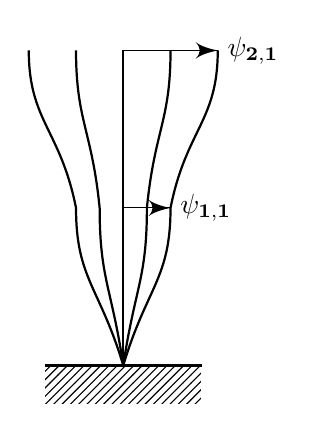
\begin{tikzpicture}
    %podloga
    \draw[white, pattern=north east lines, pattern color=black] (-1, 0)
        rectangle (1, -0.5);
    \draw[thick] (-1, 0) -- (1, 0);

    %centar
    \draw[thick] (0, 0) -- (0, 4);

    %prva
    \draw[thick] (0,0) ..controls (0.3, 1) and (0.6, 1.1).. (0.6, 2);
    \draw[thick] (0.6, 2) ..controls (0.8, 3) and (1.2, 3.1).. (1.2, 4);

    %simetricno
    \draw[thick] (0,0) ..controls (-0.3, 1) and (-0.6, 1.1).. (-0.6, 2);
    \draw[thick] (-0.6, 2) ..controls (-0.8, 3) and (-1.2, 3.1).. (-1.2, 4);

    %druga
    \draw[thick] (0,0) ..controls(0.15, 1) and (0.3, 1.1) .. (0.3, 2);
    \draw[thick] (0.3, 2) ..controls (0.4, 3) and (0.6, 3.1) .. (0.6, 4);

    %simetricno
    \draw[thick] (0,0) ..controls(-0.15, 1) and (-0.3, 1.1) .. (-0.3, 2);
    \draw[thick] (-0.3, 2) ..controls (-0.4, 3) and (-0.6, 3.1) .. (-0.6, 4);

    %vektori
    \draw[strelica1] (0, 2) -- (0.6, 2) node[pos=1,right] {$\mathbf{\psi_{1,1}}$};
    \draw[strelica1] (0, 4) -- (1.2, 4) node[pos=1,right] {$\mathbf{\psi_{2,1}}$};

\end{tikzpicture}

        \caption{Prvi vlastiti oblik titranja}
    \end{subfigure}
    \begin{subfigure}[b]{0.4\textwidth}
        \centering
        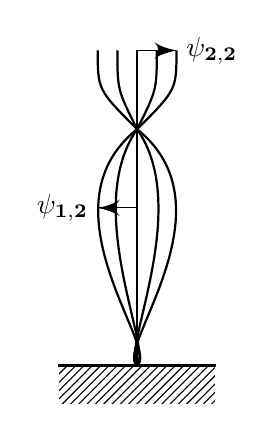
\begin{tikzpicture}
    %podloga
    \draw[white, pattern=north east lines, pattern color=black] (-1, 0)
        rectangle (1, -0.5);
    \draw[thick] (-1, 0) -- (1, 0);

    %centar
    \draw[thick] (0, 0) -- (0, 4);

    %bezier #1
%    \draw[thick] (0,0) ..controls(1.5, 2) and (-0.3,3).. (-0.5, 4);
%    \draw[thick] (0,0) ..controls(-1.5, 2) and (0.3,3).. (0.5, 4);

    \draw[thick] (0, 0) ..controls (0.3, 0.2) and (-1.25, 2) .. (0, 3);
    \draw[thick] (0, 3) ..controls (0.5, 3.5) .. (0.5, 4);

    %simietricno
    \draw[thick] (0, 0) ..controls (-0.3, 0.2) and (1.25, 2) .. (0, 3);
    \draw[thick] (0, 3) ..controls (-0.5, 3.5) .. (-0.5, 4);


    %dvica
    \draw[thick] (0, 0) ..controls (0.2, 0.2) and (-0.7, 2) .. (0, 3);
    \draw[thick] (0, 3) ..controls (0.25, 3.5) .. (0.25, 4);

    %simetricno
    \draw[thick] (0, 0) ..controls (-0.2, 0.2) and (0.7, 2) .. (0, 3);
    \draw[thick] (0, 3) ..controls (-0.25, 3.5) .. (-0.25, 4);

    %vektori
    \draw[strelica1] (0, 2) -- (-0.5, 2) node[pos=1, left] {$\mathbf{\psi_{1,2}}$};
    \draw[strelica1] (0, 4) -- (0.5, 4) node[pos=1, right] {$\mathbf{\psi_{2,2}}$};
\end{tikzpicture}

        \caption{Drugi vlastiti oblik titranja}
    \end{subfigure}
    \caption{Shematski prikaz vlastitih oblika titranja sustava s dva stupnja slobode}
\end{figure}

    \newpage
    \section{Ortogonalnost vlastitih vektora}
Kao što je već pokazano, oblike osciliranja definiraju vlastiti vektori. Dva vektora su
međusobno ortogonalna (okomita) ukoliko je njihov skalarni produkt jednak nuli.
Razmotrimo li $r$-ti i $n$-ti vlastiti vektor sustava, dobijemo slijedeći sustav jednadžbi 
(iz \eqref{eq:sustav_diferencijalnih_matricni_kratko}):
\begin{equation}\label{eq:pocetni_sustav_ortogonalnost}
    \begin{dcases}
        (\kk-\omega_r^2\mm)\vtor{\psi}{}_r=\vtor{0}{}\\
        (\kk-\omega_n^2\mm)\vtor{\psi}{}_n=\vtor{0}{}
    \end{dcases}
\end{equation}

Donju jednadžbu pomnožimo s $\vtor{\psi}{}_r^T$. U gornjoj jednadžbi prvo
transponiramo $\vtor{\psi}{}_r$ te ju pomnožimo s $\vtor{\psi}{}_n$. Sustav jednadžbi
\eqref{eq:pocetni_sustav_ortogonalnost} postaje:
\begin{equation}\label{eq:konacni_sustav_ortogonalnost}
    \begin{dcases}
        \vtor{\psi}{}_r^T(\kk-\omega_r^2\mm)\vtor{\psi}{}_n=0\\
        \vtor{\psi}{}_r^T(\kk-\omega_n^2\mm)\vtor{\psi}{}_n=0
    \end{dcases}
\end{equation}

Oduzimanjem gornje i donje jednadžbe dobijemo:
\begin{equation}
    (\omega_n^2-\omega_r^2)\vtor{\psi}{}_r^T\mm\vtor{\psi}{}_n=0
\end{equation}

Za $\omega_n\neq\omega_r$ vrijedi:
\begin{equation}\label{eq:ortogonalnost_masa}
    \vtor{\psi}{}_r^T\mm\vtor{\psi}{}_n=0
\end{equation}

Uvrštavanjem $\vtor{\psi}{}_r^T\mm\vtor{\psi}{}_n=0$ u bilo koju od jednadžbi iz
\eqref{eq:konacni_sustav_ortogonalnost} dobijemo:
\begin{equation}\label{eq:ortogonalnost_krutost}
    \vtor{\psi}{}_r^T\kk\vtor{\psi}{}_n=0
\end{equation}

Jednadžbe pod \eqref{eq:ortogonalnost_masa} i \eqref{eq:ortogonalnost_krutost}
govore da su vlastiti vektori m-ortogonalni i k-ortogonalni. Odnosno, kažemo da su
vlastiti vektori međusobno ortogonalni s obzirom na matricu mase ili matricu
krutosti. 
\par

Poslijedica ortogonalnosti su slijedeće dijagonalne pravokutne matrice:
\begin{alignat}{2}
    &\text{Modalna krutost}\quad & \mathbf{K}&=\ppsi^T\kk\ppsi\label{eq:modalna_krutost_matrica}\\
    &\text{Modalna masa}\quad &\mathbf{M}&=\ppsi^T\mm\ppsi\label{eq:modalna_masa_matrica}
\end{alignat}

Članovi na dijagonali računaju se prema slijedećim formulama:
\begin{alignat}{2}
    &\text{Za modalnu krutost}\quad & K_{n,n}&=\vtor{\psi}{}_n^Tk\vtor{\psi}{}_n\label{eq:modalna_krutost}\\
    &\text{Za modalnu masu}\quad &M_{n,n}&=\vtor{\psi}{}_n^Tm\vtor{\psi}{}_n\label{eq:modalna_masa}
\end{alignat}

Između elemenata matrica vrijedi slijedeći odnos:
\begin{equation}
    \omega_n^2=\frac{K_n}{M_n}
\end{equation}
U matričnoj formi:
\begin{equation}
    \oomega^2=\mathbf{K}\mathbf{M}^{-1}
\end{equation}


    \newpage
    \section{Normiranje vlastitih vektora}\label{sec:normiranje}
Vlastiti vektori nisu jednoznačni jer su jednako predstavljeni vektorima dobivenim
rješenjem problema vlastitih vrijednosti i njihovim višekratnicima. Drugim riječima,
vlastiti vektor predstavljen je familijom kolinearnih vektora jer vrijedi slijedeća
jednakost (~\cite{hefangfu2001})(iz \eqref{eq:vlastite_vrijednosti})
\[
    \begin{aligned}
        \kk(a\vtor{\psi}{}_n)&=\omega_n^2(a\vtor{\psi}{}_n)\mm\\
        a\kk\vtor{\psi}{}_n&=a\omega_n^2\vtor{\psi}{}_n\mm\\
        \kk\vtor{\psi}{}_n&=\omega_n^2\vtor{\psi}{}_n\mm
    \end{aligned}
\]

Množenje vlastitog vektora skalarom, s ciljem postizanja željenog oblika vlastitog
vektora, naziva se normiranje. Primjerice, željeni oblik modalnog vektora može biti 
vektor čiji je najveći element jedan:
\[
    \vtor{\psi}{}=
        \begin{Bmatrix}
            \ffrac{1}{2}\\[8pt]
            \ffrac{3}{4}
        \end{Bmatrix}
\]
Množenjem vektora s $4/3$ dobijemo:
\[
    \vtor{\psi}{}=
        \begin{Bmatrix}
            \ffrac{2}{3}\\[6pt]
            1
        \end{Bmatrix}
\]

Od posebnog značaja je normiranje modalne mase na jediničnu vrijednost. Kako je
$\vtor{\psi}{}_n^T\mm\vtor{\psi}{}_n=\mathbf{M}_{n,n}$, vlastiti vektor $\vtor{\psi}{}_n$
potrebno je množiti sa $(M_{n,n})^{-1/2}$, odnosno:
\begin{equation}\label{eq:normiranje_masa}
    \vtor{\psi}{}_n^N=\frac{1}{\sqrt{M_{n,n}}}\vtor{\psi}{}_n
\end{equation}

Gdje je $\vtor{\psi}{}_n^N$ normirani $n$-ti vlastiti vektor. Jednadžba
\eqref{eq:normiranje_masa} zapisana u matričnoj formi glasi:
\begin{equation}\label{eq:normiranje_masa_matricno}
    \ppsi_n^N=\ppsi\,\mathbf{M}^{-\frac{1}{2}}
\end{equation}

Normiranje na jediničnu vrijednost jest u biti:
\begin{equation}\label{eq:relacija_normirani}
        M_{n,n}=\left(\vtor{\psi}{}_n^N\right)^T\mm\vtor{\psi}{}_n^N=1
\end{equation}

Odnosno u matričnom obliku:
\begin{equation}\label{eq:relacija_normirani_matricno}
    \left(\ppsi^N\right)^T\mm\ppsi^N=\text{I}
\end{equation}

Gdje je I jedinična matrica. Iz \eqref{eq:modalna_krutost} slijedi:
\begin{equation}
    \begin{split}
        \left(\ppsi^N\right)^T\K\ppsi^N=\oomega^2\underbrace{\left(\ppsi^N\right)^T\M\ppsi^N}_{\text{I}} \notag\\
        \left(\ppsi^N\right)^T\K\ppsi^N=\oomega^2\label{eq:normirana_krutost}
    \end{split}
\end{equation}



    \newpage
    \section{Odziv sustava s više stupnjeva slobode na pobudu sinusnom
silom}\label{mdof_prisilne}
Kao što je pokazano u poglavlju \ref{slobodne_oscilacije}, jednadžba gibanja sustava
s $N$ stupnjeva slobode zadana je kao sustav od $N$ diferencijalnih jednadži drugog
reda. U slučaju pobude harmonijskom silom, navedeni sustav će se sastojati od $N$
nehomogenih diferencijalnih jednadžbi drugog reda, koje će biti povezane preko
matrice krutosti i/ili matrice mase. 
\par
Općenito, rješenje jedne proizvoljne nehomogene diferencijalne jednadžbe drugog reda
oblika $\alpha\ddot{y}+\beta\dot{y}+\gamma y= f(t)$ jest suma komplementarnog
rješenja $y_c$ i partikularnog rješenja $Y_p$.
\begin{equation}
    y(t)=y_c(t)+U_p(t)
\end{equation}

Komplementarno rješenje dobijemo izjednačavanjem diferencijalne jednadžbe s nulom
odnosno:
\begin{equation}\label{eq:opce_komplementarno_rjesenje}
    \alpha\ddot{y}+\beta\dot{y}+\gamma y=0
\end{equation}

Primjetimo da je komplementarno rješenje (rješenje jednadžbe \eqref{eq:opce_komplementarno_rjesenje}) 
zapravo rješenje homogene diferencijalne jednadžbe, a jednako je i za slobodne 
oscilacije i za prisilne oscilacije. Kod prisilnih oscilacija, komplementarno 
rješenje predstavlja prolazni dio odziva. Partikularno riješenje možemo pronaći 
koristeći se metodom neodređenih koeficijenata, a predstavlja prolazni dio odziva.
\par

Analogno tome, komplementarno rješenje sustava diferencijalnih jednadžbi dato je u
\eqref{eq:opce_rjesenje_sustava} te predstavlja prolazni dio odziva, pa u slučaju
prisilnih oscilacija preostaje nam odrediti još partikularno rješenje koje
predstavlja prisilni dio odziva. 
\par

Zadana je jednadžba gibanja sustava s dva stupnja slobode prikazanog na slijedećoj
slici

\textbf{UBACI SLIKU SUSTAVA}

\begin{equation}\label{eq:jednadzba_gibanja_matricno}
    \begin{bmatrix}
        m_1 & 0 \\
        0   & m_2
    \end{bmatrix}
    \begin{Bmatrix}
        \ddot{u}_1\\
        \ddot{u}_2
    \end{Bmatrix}
    +
    \begin{bmatrix}
        k_1+k_2 & -k_2\\
        -k_2 & k_2
    \end{bmatrix}
    \begin{Bmatrix}
        u_1\\
        u_2
    \end{Bmatrix}
    =
    \begin{Bmatrix}
        p_0\\
        0 
    \end{Bmatrix}
    \sin(\omega t)
\end{equation}

Odnosno:
\begin{equation}\label{eq:jednadzba_gibanja_matricno_kratko}
    \mm\vtor{u}{:}+k\vtor{u}{}=\vtor{p_n}{}\sin(\omega t)
\end{equation}

Gdje je $\vtor{p_n}{}$ vektor amplituda harmonijskih sila. Odziv sustava biti će
harmonijski, jednake frekvencije, pa partikularno rješenje možemo pretpostaviti:
\begin{equation}\label{eq:partikularno_pretpostavka}
    \vtor{u_p(t)}{}=\vtor{U_n}{}\sin(\omega t)
\end{equation}
Gdje je $\vtor{U_n}{}$ vektor koeficijenata.
Druga derivacija \eqref{eq:partikularno_pretpostavka} glasi:
\begin{equation}\label{eq:partikularno_pretpostavka_dd}
    \{\ddot{u}(t)\}=-\omega^2\vtor{U_n}{}\sin(\omega t)
\end{equation}

Uvrštavanjem \eqref{eq:partikularno_pretpostavka} i \eqref{eq:partikularno_pretpostavka_dd}
u \eqref{eq:jednadzba_gibanja_matricno_kratko} dobijemo:
\begin{equation}\label{eq:neodredjeni_koeficijenti_1}
    -\omega^2\vtor{U_n}{}\mm\sin(\omega t) 
    +
    \vtor{U_n}{}\kk\sin(\omega t)
    =
    \vtor{p}{}\sin(\omega t)
\end{equation}

Nakon sređivanja, jednadžba \eqref{eq:neodredjeni_koeficijenti_1} poprima oblik:
\begin{equation}\label{eq:neodredjeni_koeficijenti_2}
    [\kk-\omega^2\mm]\vtor{U_n}{}=\vtor{p}{}
\end{equation}

%Matrica $[\kk-\omega^2\mm]$ predstavlja matricu dinamičke krutosti sustava s više stupnjeva
%slobode, a označava se kao $[Z(\omega)]$. Jednadžbu pod \eqref{eq:neodredjeni_koeficijenti_2}
%možemo zapisati kao:
%\begin{equation}\label{eq:neodredjeni_koeficijenti_z}
%    [Z(\omega)]\vtor{U_n}{}=\vtor{p_n}{}
%\end{equation}
%
%Konačno, vektor koeficijenata dobijemo množenjem izraza \eqref{eq:neodredjeni_koeficijenti_z}
%inversom matrice dinamičke krutosti, te dobijemo:
%\begin{equation}
%    \vtor{U_n}{}=\vtor{p_n}{}\,[Z(\omega)]^{-1}
%\end{equation}

Množenjem jednadžbe \eqref{eq:neodredjeni_koeficijenti_2} s $[\kk-\omega^2\mm]^{-1}$
dobijemo:
\begin{equation}
    \begin{split}
        \vtor{U_n}{}=[\kk-\omega^2\mm]^{-1}\vtor{p_n}{} \notag\\
        \vtor{U_n}{}=\frac{1}{det[\kk-\omega^2\mm]}adj[\kk-\omega^2\mm]\vtor{p_n}{}\label{eqneodredjeni_koeficijenti_3}
    \end{split}
\end{equation}

Odnosno u matričnom obliku:
\begin{equation}
    \begin{Bmatrix}
        U_1\\
        U_2
    \end{Bmatrix}
    =
    \frac{1}{det[\kk-\omega^2\mm]}
        \begin{bmatrix}
            k_2-m_2\omega^2 & k_2\\
            k_2 & k_1+k_2-m_1\omega^2
        \end{bmatrix}
        \begin{Bmatrix}
            p_0\\
            0
        \end{Bmatrix}
\end{equation}

Komponente vektora $\vtor{U_n}{}$ glase:
\begin{align}
    U_1=\frac{p_0(k_2-m_2\omega^2)}{m_1m_2(\omega^2-\omega_1^2)(\omega^2-\omega_2^2)} \label{eq:vtor_1_opce}\\
    U_2=\frac{p_0k_2}{m_1m_2(\omega^2-\omega_1^2)(\omega^2-\omega_2^2)}\label{eq:vtor_2_opce}
\end{align}

Za $m_1=2m$, $m_2=m$, $k_1=2k$ i $k_2=k$ vektori glase:
\begin{align}
    U_1=\frac{p_0(k-m\omega^2)}{2m^2(\omega^2-\omega_1^2)(\omega^2-\omega_2^2)}\label{eq:vtor_1}\\
    U_2=\frac{p_0k}{2m^2(\omega^2-\omega_1^2)(\omega^2-\omega_2^2)}\label{eq:vtor_2}
\end{align}

Uz $\omega_1=\sqrt{k/2m}$ i $\omega_2=\sqrt{2k/m}$ te dijeljenjem \eqref{eq:vtor_1} i \eqref{eq:vtor_2}
dobijemo vektor dinamičkog koeficijenta pomaka (bez dimenzija), koji ovisi o
omjerima frekvencija $\omega/\omega_1$ te $\omega/\omega_2$. Vektor je prikazan u nastavku
\begin{equation}
    \frac{2k}{p_0}\vtor{U}{}
    =
    \begin{Bmatrix}
        \ffrac{1-0.5(\omega/\omega_1)^2}
              {[1-(\omega/\omega_1)^2][1-(\omega/\omega_2)^2]}\\[12pt]
        \ffrac{1}
              {[1-(\omega/\omega_1)^2][1-(\omega/\omega_2)^2]}
    \end{Bmatrix}
\end{equation}

Prisilni dio odziva glasi:
\begin{equation}
    \vtor{u(t)}{} = \vtor{U}{}\sin(\omega t) = 
    \begin{Bmatrix}
        \ffrac{1-0.5(\omega/\omega_1)^2}
              {[1-(\omega/\omega_1)^2][1-(\omega/\omega_2)^2]}\\[12pt]
        \ffrac{1}
              {[1-(\omega/\omega_1)^2][1-(\omega/\omega_2)^2]}
    \end{Bmatrix}
    \sin(\omega t)
\end{equation}

Komponente vektora $\vtor{U}{}$ možemo iscrtati kao graf funkcije dinamičkog faktora
$U_1/p_0/2k$ i $U_2/p_0/2k$ u ovisnosti o frekvencijskom omjeru $\omega/\omega_1$.

\section{Interesantan postupak za rješavanje 2dof}
Zadana je jednadžba gibanja prisilnog titranja sustava s dva stupnja slobode.
\begin{equation}\label{eq:jdn_gibanja_osnovno}
    \mm\vtor{u}{:}+\kk\vtor{u}{}=\vtor{p}{}\sin(\omega t)
\end{equation}

Odziv sustava će biti sinusni, iste frekvencije kao i pobuda, pa rješenje
pretpostavljamo u slijedećem obliku:
\begin{equation}\label{eq:pretpostavljeno}
    \vtor{U_p}{}=\vtor{U}{}\sin(\omega t)
\end{equation}

Druga derivacija pretpostavljenog rješenja glasi:
\begin{equation}\label{eq:pretpostavljeno_dd}
    \vtor{U_p}{}=-\omega^2\vtor{U}{}\sin(\omega t)
\end{equation}

Uvrštavanjem \eqref{eq:pretpostavljeno} i \eqref{eq:pretpostavljeno_dd} u
\eqref{eq:jdn_gibanja_osnovno} dobijemo:
\begin{equation}
    -\omega^2\vtor{U}{}\mm\sin(\omega t) + \mm\vtor{U}{}\sin(\omega t) = \vtor{p}{}\sin(\omega t)
\end{equation}

Te nakon sređivanja:
\begin{equation}\label{eq:jdn_gibanja_part_1}
    [\kk-\omega^2\mm]\vtor{U}{}=\vtor{p}{}
\end{equation}

Matrica $[\kk-\omega^2\mm]$ predstavlja matricu dinamičke krutosti.
\begin{equation}\label{eq:mat_din_krutost}
    [\kk-\omega^2\mm]=\mathbf{Z}
\end{equation}

Da bismo rješili \eqref{eq:jdn_gibanja_part_1} potrebno je pronaći invers matrice
dinamičke krutosti. Invers matrice dinamičke krutosti predstavlja matrica
frekvencijskih funkcija odziva, a označavamo ju s $\mathbf{H}$. Jednadžba pod 
\eqref{eq:mat_din_krutost} može poprimiti slijedeći oblik:
\begin{equation}
    \left(\ppsi^N\right)^T[\kk-\omega^2\mm]\ppsi^N
    =
    \left(\ppsi^N\right)^T\mathbf{Z}\;\ppsi^T
\end{equation}
Odnosno
\begin{equation}
     \left(\ppsi^N\right)^T[\kk-\omega^2\mm]\ppsi^N
    =
    \left(\ppsi^N\right)^T\mathbf{H}^{-1}\;\ppsi^T
\end{equation}

Iz \eqref{eq:relacija_normirani_matricno} i \eqref{eq:normirana_krutost} slijedi:
\begin{equation}
    [\omega_n^2 - \omega^2] = \left(\ppsi^N\right)^T\mathbf{H}^{-1}\;\ppsi^T
\end{equation}

Nakon sređivanja, dobijemo:
\begin{equation}
    \mathbf{H}=\left(\ppsi^N\right)^T[\omega_n^2 - \omega^2]^{-1}\;\ppsi^T
\end{equation}

Član $H_{j,k}$ matrice $\mathbf{H}$ možemo dobiti preko slijedeće jednadžbe:
\begin{equation}\label{eq:clan_frf_matrice}
    H_{j,k}=\frac{\psi^N_{j,1}\psi^N_{k,1}}{\omega_1^2-\omega^2}
            +
            \frac{\psi^N_{j,2}\psi^N_{k,2}}{\omega_2^2-\omega^2}
            +
            \frac{\psi^N_{j,3}\psi^N_{k,3}}{\omega_3^2-\omega^2}
            +
            \cdots
            +
            \frac{\psi^N_{j,n}\psi^N_{k,n}}{\omega_n^2-\omega^2}
\end{equation}

Jednadžbu \eqref{eq:clan_frf_matrice} možemo zapisati kao skalarni umnožak vektora:
\begin{equation}\label{eq:clan_frf_matrica_vektorski}
    H_{j,k}
    =
    \begin{Bmatrix}
        \psi_{j,1}\psi_{k,1} &
        \psi_{j,2}\psi_{k,2} &
        \psi_{j,3}\psi_{k,3} &
        \cdots
        \psi_{j,n}\psi_{k,n}
    \end{Bmatrix}
    \begin{Bmatrix}
        \ffrac{1}{\omega_1^2-\omega^2}\\[6pt]
        \ffrac{1}{\omega_2^2-\omega^2}\\[6pt]
        \ffrac{1}{\omega_3^2-\omega^2}\\[6pt]
        \vdots\\[6pt]
        \ffrac{1}{\omega_n^2-\omega^2}
    \end{Bmatrix}
\end{equation}

Za zadani sustav, matrica modova normiranih s obzirom na masu $\ppsi^N$ glasi:
\[
    \ppsi^N
    =
    \begin{Bmatrix}
        \ffrac{\sqrt{6m}}{6m} & -\ffrac{\sqrt{3m}}{3m}\\[12pt]
        \ffrac{\sqrt{6m}}{6m} & \ffrac{\sqrt{3m}}{3m}
    \end{Bmatrix}
\]

Izračun matrice frekvencijske funkcije odziva $H_{1,1}$ prikazan je u nastavku:
\[
\begin{aligned}
    H_{1,1} &=
    \frac{\psi^N_{1,1}}{\omega_1^2-\omega^2}+\frac{\psi^N_{1,1}}{\omega_2^2-\omega^2}
    =
    \frac{\ffrac{\sqrt{6m}}{6m}\ffrac{\sqrt{6m}}{6m}}{\omega_1^2-\omega^2}
    +
    \frac{\ffrac{\sqrt{3m}}{3m}\ffrac{\sqrt{3m}}{3m}}{\omega_2^2-\omega^2}\\
    %
    H_{1,1} &=
    \frac{1}{3m} 
        \left(
            \frac{\ffrac{1}{2}}{(\omega_1^2-\omega^2}
            +
            \frac{1}{(\omega_2^2-\omega^2)}
        \right)
    =
    \frac{1}{3m}
        \left(
            \frac{\ffrac{1}{2}(\omega_2^2-\omega^2)+(\omega_1^2-\omega^2)}
                {\omega_1^2\omega_2^2(1-(\omega/\omega_1)^2)(1-(\omega/\omega_2)^2}
        \right)\\
\end{aligned}
\]

U brojniku, $\omega_2$ izrazimo kao $\omega_1$ pomoću relacije $\omega_2=\sqrt{2k/m}$
i $\omega_1=\sqrt{k/2m}$.
\[
    \begin{aligned}
        H_{1,1}=
        \frac{1}{3m}
            \left(
                \frac{3-\ffrac{3}{2}(\omega/\omega_1)^2}
                    {\omega_2^2(1-(\omega/\omega_1)^2)(1-(\omega/\omega_2)^2)}
            \right)
    \end{aligned}
\]
Nakon sređivanja:
\begin{equation}\label{eq:frf_11}
    H_{1,1}=\frac{1-\ffrac{1}{2}(\omega/\omega_1)^2}{2k(1-(\omega_1/\omega)^2)(1-(\omega_2/\omega)^2)}
\end{equation}

Analogno tome, dobiju se ostali članovi matrice te glase:
\begin{align}
    H_{1,2} &= \frac{1}{2k(1-(\omega_1/\omega)^2)(1-(\omega_2/\omega)^2)}\label{eq:frf_12}\\
    H_{2,1} &= \frac{1}{2k(1-(\omega_1/\omega)^2)(1-(\omega_2/\omega)^2)}\label{eq:frf_21}\\
    H_{2,2} &= \frac{1-2(\omega/\omega_2)^2}{2k(1-(\omega_1/\omega)^2)(1-(\omega_2/\omega)^2)}\label{eq:frf_22}\\
\end{align}

Matrica $\mathbf{H}$ glasi:
\begin{equation}\label{eq:matrica_frf}
    \mathbf{H}=\frac{1}{2k(1-(\omega/\omega_1)^2(1-(\omega/\omega_2)^2)}
    \begin{bmatrix}
        1-\ffrac{1}{2}\left(\ffrac{\omega}{\omega_1}\right)^2 & 1 \\
        1 & 1-2\left(\ffrac{\omega}{\omega_2}\right)^2
    \end{bmatrix}
\end{equation}

Uvrštavanjem \eqref{eq:matrica_frf} u \eqref{eq:jdn_gibanja_part_1} dobijemo:
\begin{equation}
    \mathbf{H}^{-1}\vtor{U}{}=\vtor{p}{}
\end{equation}

Množenjem prethodnog izraza s $\mathbf{H}$:
\begin{equation}
    \vtor{U}{} = \mathbf{H}\vtor{p}{}
\end{equation}

Raspisivanjem prethodne jednadžbe:
\begin{equation}
    \begin{Bmatrix}
        U_1\\
        U_2
    \end{Bmatrix}
    =
    \frac{1}{2k\left(1-\left(\ffrac{\omega_1}{\omega}\right)^2\right)\left(1-\left(\ffrac{\omega_2}{\omega}\right)^2\right)}
    %
    \begin{bmatrix}
        1-\ffrac{1}{2}\left(\ffrac{\omega}{\omega_1}\right)^2 & 1 \\
        1 & 1-2\left(\ffrac{\omega}{\omega_2}\right)^2
    \end{bmatrix}
    % 
    \begin{Bmatrix}
        p_0\\
        0
    \end{Bmatrix}
\end{equation}

Te konačno, vektor $\vtor{U}{}$ glasi:
\begin{equation}\label{eq:vektor_u_konacno}
    \begin{Bmatrix}
        U_1\\
        U_2
    \end{Bmatrix}
    =
    \frac{1}{2k\left(1-\left(\ffrac{\omega_1}{\omega}\right)^2\right)\left(1-\left(\ffrac{\omega_2}{\omega}\right)^2\right)}
    \begin{Bmatrix}
        p_0\left(1-\ffrac{1}{2}\left(\ffrac{\omega}{\omega_1}\right)^2\right)\\
        p_0 
    \end{Bmatrix}
\end{equation}

Dijeljenjem vektora $\vtor{U}{}$ s $p_0/2k$ dobijemo slijedeće:
\begin{equation}
    \begin{Bmatrix}
        U_1\\
        U_2
    \end{Bmatrix}
    =
    \frac{1}{\left(1-\left(\ffrac{\omega_1}{\omega}\right)^2\right)\left(1-\left(\ffrac{\omega_2}{\omega}\right)^2\right)}
    \begin{Bmatrix}
        1-\ffrac{1}{2}\left(\ffrac{\omega}{\omega_1}\right)^2\\
        1 
    \end{Bmatrix}
\end{equation}

%Komponente vektora zapisane posebno:
%\begin{align}
%    U_1&=\frac{1-\ffrac{1}{2}\left(\ffrac{\omega}{\omega_1}\right)^2}
%        {\left(1-\left(\ffrac{\omega_1}{\omega}\right)^2\right)\left(1-\left(\ffrac{\omega_2}{\omega}\right)^2\right)}\\
%    U_2&=\frac{1}{\left(1-\left(\ffrac{\omega_1}{\omega}\right)^2\right)\left(1-\left(\ffrac{\omega_2}{\omega}\right)^2\right)}
%\end{align}

Komponente vektora $U$ predstavljaju funkcije ovisnosti dinamičkog faktora o 
frekvencijskim omjerima $\omega/\omega_1$ i $\omega/\omega_2$. Njihovi grafovi
prikazani su u nastavku.

\textbf{UBACI GRAFOVE}

Prisilni dio odziva glasi:
\begin{equation}
    \begin{split}
        \vtor{u(t)}{} = \vtor{U}{}\; sin(\omega t)
        %\vtor{u(t)}{}=
        =
        \frac{1}{\left(1-\left(\ffrac{\omega_1}{\omega}\right)^2\right)\left(1-\left(\ffrac{\omega_2}{\omega}\right)^2\right)}
    \begin{Bmatrix}
        1-\ffrac{1}{2}\left(\ffrac{\omega}{\omega_1}\right)^2\\
        1 
    \end{Bmatrix}
    \sin(\omega t)
    \end{split}
\end{equation}


    \newpage
    \section{Modalna analiza}\label{sec:modalnaAnalizaNepriguseniSustav}
Modalna analiza je postupak određivanja osnovnih dinamičkih parametara linearnog
sustava s ciljem definiranja matematičkog modela ponašanja sustava pod utjecajem
dinamičkih sila. Modalna analiza temelji se na \textit{principu superpozicije},
odnosno na činjenici da se ukupni odziv sustava može zapisati kao linearna
kombinacija odziva pojedinih oblika titranja.
\par

Razmotrimo jednadžbu gibanja sustava s više stupnjeva slobode pobuđenog proizvoljnom
silom:
\begin{equation}\label{eq:mdof_jdn_gibanja_opca_pobuda}
    \mm\vtor{u}{:} + \kk\vtor{u}{} = \vtor{p(t)}{}
\end{equation}

Klasično rješenje jednadžbe gibanja \eqref{eq:mdof_jdn_gibanja_opca_pobuda}
prikazano je u poglavlju ~\ref{mdof_prisilne} na primjeru sustava s dva stupnja 
slobode pobuđenog harmonijskom silom. Za sustave s više od dva stupnja slobode ili
za složenije sile pobude, rješavanje jednadžbe gibanja na klasični način može biti
izuzetno teško ili nemoguće. U takvim slučajevima, jednadžba gibanja se rješava
postupcima modalne analize.
\par

Iz poglavlja ~\ref{slobodne_oscilacije} znamo da je rješenje jednadžbe gibanja
slobodnog titranja sustava s više stupnjeva slobode linearna kombinacija
odziva svih pojedinih oblika titranja odnosno:
\begin{equation}\label{eq:mdf_ukupno_rjesenje}
    u(t)=\sum_{r=1}^N\psi_rq_r(t)
\end{equation}

Uvrštavanjem \eqref{eq:mdf_ukupno_rjesenje} u \eqref{eq:mdof_jdn_gibanja_opca_pobuda} 
dobijemo:
\begin{equation}\label{eq:mdf_modalna_1}
    \sum_{r=1}^N\mm\psi_r\ddot{q}_r(t) + \sum_{r=1}^N\kk\psi_rq_r(t)=p(t)
\end{equation}

Množenjem jednadžbe \eqref{eq:mdf_modalna_1} s $\psi_n^T$ dobijemo:
\begin{equation}\label{eq:mdf_modalna_2}
    \sum_{r=1}^N\psi_n^T\mm\psi_r\ddot{q}_r(t)+\sum_{r=1}^N\psi_n^T\kk\psi_rq_r(t)=\psi_n^Tp(t)
\end{equation}

Zbog svojstva ortogonalnosti, isčezavaju svi članovi sumacija osim $n$-tog člana, pa
preostaje:
\begin{equation}\label{eq:mdf_modalna_jednadzba_nesredjeno}
    \psi_n^T\,\mm\,\psi_n\,\ddot{q}_n(t)\;+\;\psi_n^T\,\kk\,\psi_n\,q_r(t)=\psi_n^T\,p(t)
\end{equation}

Koristeći relacije iz \eqref{eq:modalna_masa} i \eqref{eq:modalna_krutost} jednadžba
\eqref{eq:mdf_modalna_jednadzba_nesredjeno} poprima slijedeći oblik:
\begin{equation}\label{eq:mdf_modalna_jednadzba_sredjeno}
    M_n\ddot{q}_n(t)+K_nq_n(t)=P_n(t)
\end{equation}

Gdje su $M_n$, $K_n$ i $P_n$ poopćena masa, krutost i opterećenje $n$-tog modalnog
oblika.

Postupkom, prikazanim u jednadžbama \eqref{eq:mdf_ukupno_rjesenje},
\eqref{eq:mdf_modalna_1}, \eqref{eq:mdf_modalna_2},
\eqref{eq:mdf_modalna_jednadzba_nesredjeno}, jednadžbu gibanja sustava predstavljenu
sustavom diferencijalnih jednadžbi sveli smo na skup međusobno neovisnih
diferencijalnih jednadžbi. Drugim riječima, sustav od $N$ stupnjeva slobode razložen
je na $N$ međusobno neovisnih podsustava s jednim stupnjem slobode (princip superpozicije), 
pri čemu $n$-ti podsustav prikazuje odziv sustava u $n$-tom modu. Podsustave 
nazivamo \textit{poopćeni sustav za n-ti oblik titranja}. "Jednadžba gibanja" 
poopćenog sustava za $n$-ti oblik titranja predstavljena je diferencijalnom jednadžbom
\eqref{eq:mdf_modalna_jednadzba_sredjeno} čije rješenje predstavlja modalnu 
koordinatu $n$-tog oblika titranja $q_n(t)$.
\par

Odziv $n$-tog oblika titranja je:
\begin{equation}\label{eq:mdf_odziv_ntog_moda}
    \vtor{u_n(t)}{}=\vtor{\psi}{}_nq_n(t)
\end{equation}

Da bismo odredili ukupni odziv sustava s $N$-stupnjeva slobode, potrebno je riješiti
$N$ modalnih jednadžbi, oblika definiranog pod \eqref{eq:mdf_modalna_jednadzba_sredjeno}.
Matrični zapis sustava modalnih jednadžbi prikazan je u nastavku.
\begin{equation}\label{eq:sustav_modalnih_jednadzbi}
    \M\vtor{q}{:} + \K\vtor{q}{}=\vtor{P(t)}{}
\end{equation}

Gdje je $\M$ matrica modalnih masa, $\K$ matrica modalnih krutosti, $\vtor{P(t)}{}$
vektor poopćenih opterećenja. Iz \eqref{eq:modalna_masa_matrica} i
\eqref{eq:modalna_krutost_matrica} znamo da su matrice $\M$ i $\K$ dijagonalne što
znači da je \eqref{eq:sustav_modalnih_jednadzbi} sustav međusobno neovisnih jednadžbi.
Rješenjem navedenog sustava, dobijemo funkcije modalnih koordinata za sve 
oblike titranja sustava, a ukupni odziv definiran je linearnom kombinacijom 
(princip superpozicije) odziva svakog pojedinog oblika titranja. Odziv pojedinog oblika
osciliranje definiran je
\eqref{eq:mdf_odziv_ntog_moda}, a ukupni odziv je:

\begin{equation}\label{eq:mdf_modalna_ukupno_rjesenje}
    \vtor{u(t)}{}=\sum_{n=1}^N\vtor{u_n(t)}{}=\sum_{n=1}^N\vtor{\psi}{}_nq_n(t)
\end{equation}

    \newpage
    \section{Prigušenje u sustavu s više stupnjeva slobode}
Model prigušenog sustava s više stupnjeva slobode prikazan je na slijedećoj slici.
\par
\begin{figure}[H]
    \begin{subfigure}[b]{0.5\textwidth}
        \centering
        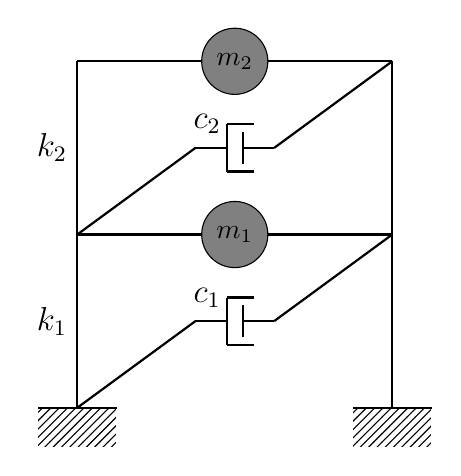
\begin{tikzpicture}
%štapovi
    %prvi (donji) okvir
	\draw[thick] (0,0) -- (0,2.2)
                node[pos=0.5,left]{\large{$k_1$}};
	\draw[thick] (0,2.2) -- (4,2.2);
	\draw[thick] (4,0) -- (4,2.2);

    %drugi (gornji) okvir
        \draw[thick] (0,2.2) -- (0, 4.4)
                node[pos=0.5,left]{\large{$k_2$}};
        \draw[thick] (0, 4.4) -- (4, 4.4);
        \draw[thick] (4, 2.2) -- (4, 4.4);
	
%mase
        %donja
	\filldraw[color=black, fill=gray] (2,2.2) circle (0.42);
	\node[draw=none, fill=none] at(2,2.2) 
        {$m_1$};

        %gornja
        \filldraw[color=black, fill=gray] (2,4.4) circle (0.42);
        \node[draw=none, fill=none] at (2,4.4)
        {$m_2$};

        %dolje
        \prigusivac{0}{0}{4}{2.2}
        \node[draw=none, fill=none] at (1.65, 1.4) {\large{$c_1$}};
        %gore
        \prigusivac{0}{2.2}{4}{4.4} 
        \node[draw=none, fill=none] at (1.65, 3.6) {\large{$c_2$}};


%podloga
	\draw[white, pattern=north east lines, pattern color=black] (-0.5, 0) 
	rectangle (0.5, -0.5);
	\draw[thick] (-0.5, 0) -- (0.5, 0);

	\draw[white, pattern=north east lines, pattern color=black] (3.5, 0)
	rectangle (4.5, -0.5);
	\draw[thick] (3.5, 0) -- (4.5, 0);
\end{tikzpicture}

        \caption{}
        \label{fig:priguseni_sustav_okvir-2dof}
    \end{subfigure}
    \hfill
    \begin{subfigure}[b]{0.5\textwidth}
        \centering
        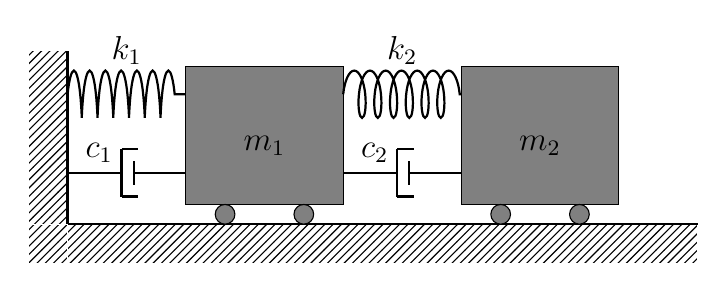
\begin{tikzpicture}
	%podloga
	\draw[white, pattern=north east lines, pattern color=black] (0, 0)
	rectangle (-0.5, 2.2);
	\draw[thick] (0,0) -- (0, 2.2);

	\draw[white, pattern=north east lines, pattern color=black] (0, 0) 
	rectangle (8, -0.5);
	\draw[thick] (0,0) -- (8,0);
	
	\draw[white, pattern=north east lines, pattern color=black] (0, 0)
	rectangle (-0.5, -0.5);

	%uteg
	\filldraw[fill=gray] (1.5, 2) rectangle (3.5, 0.25);
        \filldraw[fill=gray] (5, 2) rectangle (7, 0.25);

	%kotaci
	\filldraw[fill=gray] (2, 0.125) circle (0.125);
	\filldraw[fill=gray] (3, 0.125) circle (0.125);

        \filldraw[fill=gray] (5.5, 0.125) circle (0.125);
        \filldraw[fill=gray] (6.5, 0.125) circle (0.125);

	%opruga
	\draw[thick, decoration={aspect=0.1, segment length=2mm,amplitude=3mm,coil},decorate] (0,1.65) -- (1.5, 1.65);
        \draw[thick, decoration={aspect=0.3, segment length=2mm,amplitude=3mm,coil},decorate] (3.5, 1.65) -- (5, 1.65);

        %prigusivac 1
	\draw[thick] (0, 0.65) -- (0.685, 0.65);
	\draw[thick] (0.84, 0.65) -- (1.5, 0.65);

	\draw[thick] (0.685, 0.35) -- (0.685, 0.95);
	\draw[thick] (0.685, 0.95) -- (0.9, 0.95);
	\draw[thick] (0.685, 0.35) -- (0.9, 0.35);

	\draw[thick] (0.84, 0.5) -- (0.84, 0.8);

        %prigusivac 2 
	\draw[thick] (3.5, 0.65) -- (4.185, 0.65);
	\draw[thick] (4.34, 0.65) -- (5, 0.65);

	\draw[thick] (4.185, 0.35) -- (4.185, 0.95);
	\draw[thick] (4.185, 0.95) -- (4.4, 0.95);
	\draw[thick] (4.185, 0.35) -- (4.4, 0.35);

	\draw[thick] (4.34, 0.5) -- (4.34, 0.8);

        \node[draw=none, fill=none] at (0.75, 2.2) {\large{$k_1$}}; 
        \node[draw=none, fill=none] at (2.5,   1) {\large{$m_1$}};
        \node[draw=none, fill=none] at (0.4,  0.9) {\large{$c_1$}};

        \node[draw=none, fill=none] at (4.25, 2.2) {\large{$k_2$}};
        \node[draw=none, fill=none] at (6, 1) {\large{$m_2$}};
        \node[draw=none, fill=none] at (3.9, 0.9) {\large{$c_2$}};

\end{tikzpicture}

        \caption{}
        \label{fig:priguseni_ekvivalentni_sustav-2dof}
    \end{subfigure}
    \vfill
    \vspace{0.5cm}
    \begin{subfigure}[b]{1\textwidth}
        \centering
        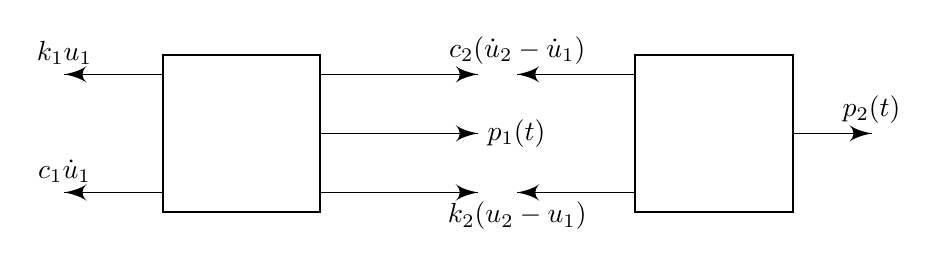
\begin{tikzpicture}
	%uteg_1
	\draw[black,thick] (1.5, 2) rectangle (3.5, 0);

	%sile
	\draw[strelica1] (1.5, 1.75) -- (0.25, 1.75) 
		node[pos=1, above]{$k_1u_1$};
        \draw[strelica1] (1.5, 0.25) -- (0.25, 0.25)
                node[pos=1, above]{$c_1\dot{u}_1$};

	\draw[strelica1] (3.5, 1) -- ( 5.5, 1) 
		node[pos=1, right]{$p_1(t)$};
        \draw[strelica1] (3.5, 1.75) -- (5.5, 1.75);
%                node[pos=1, below]{$k_2(u_2-u_1)$};
        \draw[strelica1] (3.5, 0.25) -- (5.5, 0.25);
%                 node[pos=1, below]{$c_2(\dot{u}_2-\dot{u}_1)$}
                 
            
        %uteg_2
        \draw[black,thick] (7.5, 2) rectangle (9.5, 0);

        %sile
        \draw[strelica1] (7.5, 1.75) -- (6, 1.75)
                node[pos=1, above] {$c_2(\dot{u}_2-\dot{u}_1)$};
        \draw[strelica1] (7.5, 0.25) -- (6, 0.25)
                node[pos=1, below]{$k_2(u_2-u_1)$};
        \draw[strelica1] (9.5, 1) -- (10.5, 1)
                node[pos=1, above]{$p_2(t)$};

\end{tikzpicture}

        \caption{}
        \label{fig:priguseni_sustav_okvir_sile-2dof}
    \end{subfigure}
    \caption{Idealizirani sustav s dva stupnja slobode i prigušenjem:
    (\subref{fig:priguseni_sustav_okvir-2dof}) dvoetažni posmični okvir s prigušenjem;
    (\subref{fig:priguseni_ekvivalentni_sustav-2dof}) ekvivalentni prigušeni model;
    (\subref{fig:priguseni_sustav_okvir_sile-2dof}) prikaz sila; } 
    \label{fig:priguseni_sustav-2dof}
\end{figure}

Jednadžba gibanja sa slike \ref{fig:priguseni_sustav-2dof} glasi:
\begin{equation}\label{eq:JednadzbaGibanjaPriguseniMDF}
    \begin{dcases}
        m_1\ddot{u}_1+\dot{u}_1(c_1+c_2)-c_2\dot{u}_2+u_1(k_1+k_2)-k_2u_2=p_1(t)\\
        m_2\ddot{u}_2+c_2\dot{u}_2-c_2\dot{u}_1+k_2u_2-k_2u_1=p_2(t)
    \end{dcases}
\end{equation}

Sustav \eqref{eq:JednadzbaGibanjaPriguseniMDF} možemo zapisati u matričnom obliku:
\begin{equation}\label{eq:JednadzbaGibanjaPriguseniMDF-matrice}
    \begin{bmatrix}
        m_1 & 0 \\
        0   & m_2
    \end{bmatrix}
    \begin{Bmatrix}
        \ddot{u}_1\\
        \ddot{u}_2
    \end{Bmatrix}
    +
    \begin{bmatrix}
        c_1 + c_2 & -c_2\\
        -c_2 & c_2
    \end{bmatrix}
    +
    \begin{bmatrix}
        k_1+k_2 & -k_2\\
        -k_2 & k_2
    \end{bmatrix}
    \begin{Bmatrix}
        u_1\\
        u_2
    \end{Bmatrix}
    =
    \begin{Bmatrix}
        p_1\\
        p_2 
    \end{Bmatrix}
\end{equation}

Kompaktniji zapis jednadžbe pod \eqref{eq:JednadzbaGibanjaPriguseniMDF-matrice} 
prikazan je u nastavku:
\begin{equation}\label{eq:JednadzbaGibanjaPrigusenoMDF-matricni}
    \mm\vtor{u}{:}+\cc\vtor{u}{.}+\kk\vtor{u}{} = \vtor{p}{}
\end{equation}

Uvodi se $u=\ppsi\vtor{q}{}$ te jednadzba \eqref{eq:JednadzbaGibanjaPrigusenoMDF-matricni}
poprima slijedeći oblik:
\begin{equation}
    \mm\ppsi\vtor{q}{:}+\cc\ppsi\vtor{q}{.}+\kk\ppsi\vtor{q}{}=\vtor{p(t)}{}\qquad 
\end{equation}

Množenjem s $\ppsi^T$ dobijemo:
\begin{equation}\label{eq:JednadzbaGibanjaPrigusenoMDF-svedi}
    \ppsi^T\mm\ppsi\vtor{q}{:}+\ppsi^T\cc\ppsi\vtor{q}{.}+\ppsi^T\kk\ppsi\vtor{q}{}=\ppsi^T\vtor{p(t)}{}\\
\end{equation}

Iz poglavlja \ref{sec:normiranje} poznato je da vrijedi:
\begin{align*}
    \M &= \ppsi^T\mm\ppsi\\
    \K &= \ppsi^T\kk\ppsi
\end{align*}
Gdje su matrice $\M$ i $\K$ dijagonalne matrice modalne mase odnosno krutosti. Osim
matrica $\M$ i $\K$ uvodi se i matrica $\C$ koju nazivamo matricom modalnog
prigušenja, pa je jednadžbu \eqref{eq:JednadzbaGibanjaPrigusenoMDF-svedi} moguće
zapisati na slijedeći način:

\begin{equation}\label{eq:ModalneJednadzbe}
    \M\vtor{q}{:} + \C\vtor{q}{.} + \K\vtor{q}{} = \vtor{P}{}
\end{equation}

Gdje je $\vtor{P}{}$ vektor modalnog opterećenja. Matrica modalnog prigušenja $\C$ može 
i ne mora biti dijagonalna pa je potrebno razmotriti dva različita slučaja.
    \begin{enumerate}
        \item Ukoliko je matrica $\C$ dijagonalna, jednadžba
            \eqref{eq:ModalneJednadzbe} predstavlja skup međusobno neovisnih
            jednadžbi pa je na takvome sustavu primjenjiva klasična modalna analiza.
            Takav oblik prigušenja naziva se \textit{klasični oblik prigušenja}.
            
        \item Ukoliko matrica $\C$ nije dijagonalna, jednadžba
            \eqref{eq:ModalneJednadzbe} predstavlja sustav međusobno povezanih
            diferencijalnih jednadžbi, te na takav sustav nije primjenjiva klasična
            modalna analiza. Takav oblik prigušenja naziva se \textit{općim oblikom
            prigušenja}.
    \end{enumerate}

Matrica modalnog prigušenja zadana je slijedećim izrazom:
\begin{equation}\label{eq:ModalnoPrigusenje}
    C = \ppsi^T \cc \ppsi
\end{equation}

Za sustav s dva stupnja slobode, matrica $\C$ glasi:
\begin{equation}
    \begin{bmatrix}
        I & II\\
        III & IV
    \end{bmatrix}
\end{equation}

Gdje je:
\begin{align*}
    I  &= \psi_{1,1}^2c_1+\psi_{1,1}^2c_2+\psi_{2,1}c_2\psi_{1,1}+\psi_{2,1}^2c_2-\psi_{1,1}c_2\psi_{2,1}\\
    II &= \psi_{1,1}c_1\psi_{1,2}+\psi_{1,1}c_2\psi_{1,2}-\psi_{2,1}c_2\psi_{1,2}+\psi_{2,1}c_2\psi_{2,2}-\psi_{1,1}c_2\psi_{2,2}\\
    III&= \psi_{1,1}c_1\psi_{1,2}+\psi_{1,1}c_2\psi_{1,2}-\psi_{2,1}c_2\psi_{1,2}+\psi_{2,1}c_2\psi_{2,2}-\psi_{1,1}c_2\psi_{2,2}\\
    IV &= \psi_{1,2}^2c_1+\psi_{1,2}^2c_2i-\psi_{2,2}c_2\psi_{1,2}+\psi_{2,2}^2c_2-\psi_{1,2}c_2\psi_{2,2}
\end{align*}

Matrica $\C$ biti će dijagonalna ukoliko su elementi iznad i ispod glavne dijagonale
jednaki nuli, što znači da je potrebno riješiti slijedeći sustav jednadžbi:
\begin{equation}
    \begin{dcases}
        II=0\\
        III=0
    \end{dcases}
\end{equation}

Zbog toga što je matrica $\C$ simetrična s obzirom na glavnu dijagonalu (u ovom
slučaju), preostaje jedna jednadžba s dvije nepoznanice $c_1$ i $c_2$, odnosno:
\begin{equation}\label{eq:JednadzbaRazdiobaPrigusenja}
    \psi_{1,1}c_1\psi_{1,2}+\psi_{1,1}c_2\psi_{1,2}-\psi_{2,1}c_2\psi_{1,2}+\psi_{2,1}c_2\psi{2,2}-\psi_{1,1}c_2\psi_{2,2}=0
\end{equation}

Navedena jednadžba ima beskonačno mnogo rješenja slijedećeg oblika:
\begin{equation}\label{eq:JednadzbaRazdiobaPrigusenja-rjesenje}
    \frac{c_1}{c_2} = -\frac{\psi_{1,2}\psi_{1,1}-\psi_{2,2}\psi_{1,1}+\psi_{2,2}\psi_{2,1}-\psi_{1,2}\psi_{2,1}}
                            {\psi_{1,2}\psi_{1,1}}
\end{equation}

Rješenja jednadžbe \eqref{eq:JednadzbaRazdiobaPrigusenja}
predstavljaju svaki $c_1$ i $c_2$, čiji je međusobni omjer jednak razlomku s desne
strane izraza \eqref{eq:JednadzbaRazdiobaPrigusenja-rjesenje}. Iz jednadžbi
\eqref{eq:JednadzbaRazdiobaPrigusenja} i \eqref{eq:JednadzbaRazdiobaPrigusenja-rjesenje} 
slijedi da će matrica $\C$ biti dijagonalna samo ako omjer koeficijenata prigušenja $c_1/c_2$ 
zadovoljava jednakost pod \eqref{eq:JednadzbaRazdiobaPrigusenja-rjesenje}. U
protivnom, matrica $\C$ nije dijagonalna a u sustavu vlada opći oblik prigušenja.
Omjer prigušenja nazivamo \textit{razdiobom prigušenja u sustavu}. Zaključno, oblik
matrice $\C$ ovisi o razdiobi prigušenja u sustavu.
\par

Bitno je za napomenuti da u slučaju općeg prigušenja, oblici titranja sustava
su različiti od oblika titranja neprigušenog sustava, a iz jednadžbe pod
\eqref{eq:JednadzbaGibanjaPriguseniMDF-matrice} dobije se kompleksni problem
vlastitih vrijednosti čija rješenja su kompleksni vlastiti vektori $\psi$ i
kompleksne vlastite vrijednosti $\omega$. Zbog svoje dugotrajnosti i matematičke složenosti,
navedeni slučaj neće biti razmatran u ovome radu.
\par

Dakle, jednadžbu \eqref{eq:ModalneJednadzbe} moguće je riješiti ukoliko je sustav
prigušen klasičnim oblikom prigušenja (matrica $\C$ je dijagonalna), pri čemu je
postupak analogan postupku iz poglavlja ~\ref{sec:modalnaAnalizaNepriguseniSustav}. Modalna
jednadžba n-tog oblika titranja glasi:
\begin{equation}\label{eq:ModalnaJednadzba_n}
    M_n\ddot{q}_n + C_n\dot{q}_n  + K_nq = P_n(t)
\end{equation}
Gdje je $M_n$, $C_n$, $K_n$ i $P_n$ modalna masa, modalno prigušenje, modalna
krutost i modalno opterećenje n-tog oblika titranja.
Dijeljenjem jednadžbe \eqref{eq:ModalnaJednadzba_n} s modalnom masom $M_n$ dobijemo:
\begin{equation}\label{eq:modalnaPriguseno-konacno}
    \ddot{q}_n + 2\omega_n\zeta_n\ddot{q}_n + \omega_n^2q = \frac{P_n}{M_n}
\end{equation}

Gdje je $\zeta_n$ relativni faktor prigušenja n-tog oblika titranja a $\omega_n$
prirodna frekvencija n-tog oblika titranja. Forma rješenja diferencijalne jednadžbe 
\eqref{eq:modalnaPriguseno-konacno} prikazana je pod \eqref{eq:modalnaPriguseno-rjesenje} 
a predstavlja odziv n-tog oblika titranja sustava s više stupnjeva slobode. 

\begin{equation}\label{eq:modalnaPriguseno-rjesenje}
    u_n = \psi_n q_n(t)
\end{equation}

Ukupni odziv dobijemo superpozicijom odziva svih modalnih oblika, odnosno:
\begin{equation} 
    u(t) = \sum_{n=1}^Nu_n(t) = \sum_{n=1}^N\psi_nq_n(t)
\end{equation}

\chapter{Zaljučak}
    Razvojem računala i računalne tehnologije otvara se prostor za razvitak dinamike
konstrukcija. Za razumijevanje osnovnih teoretskih principa i pojmova dinamike
konstrukcija potrebno je kvalitetno poznavanje najjednostavnijeg sustava, tj.
sustava s jednim stupnjem slobode. Osim didaktičke svrhe, sustav s jednim stupnjem
slobode može poslužiti i kao model za razvitak eksperimentalnih metoda kao što je
rezonancijski pokus. 
\par

U inženjerskoj praksi vrlo često se susreću sustavi s više stupnjeva slobode koji
mogu biti izrazito složeni. U graditeljstvu sustav s više stupnjeva slobode pojavljuje
se kod visokih građevina, primjerice nebodera. Visoke građevine posebno su osjetljive
na horizontalna dinamička opterećenja, poput vjetara i potresa. 
Poznavanjem dinamičkih parametara konstrukcije, moguće je efekte dinamičkog
opterećenja svesti na minimum odnosno učinkovito dimenzionirati konstrukciju na
dinamičko opterećenje. Primjerice, dinamički parametri konstrukcije mogu se 
iskoristiti za projektiranje posebnih prigušivača koji se zatim ugrađuju na pogodna 
mjesta u konstrukciju. Dinamički parametri konstrukcija najšešće se određuju
modalnom analizom.
\par

U rudarstvu postupci modalne analize primjenjivi su na analizu odziva konzole
rotornog bagera, u separacijskim postrojenjima na analizu vibracijskih sita i sl. 
\par

Osim u graditeljstvu i rudarstvu, postupci modalne analize koriste se u brojnim tehničkim i
znanstvenim disciplinama, kao što su strojarstvo, zrakoplovno inženjerstvo, autoindustrija
i sl.
\par

Jedna od meni osobno interesantnijih primjena modalne analize je u akustici. U
akustici, modalna analiza se može koristiti za određivanje projektnih parametara
zvučnika te za otkrivanje „malih tajni velikih majstora”, na primjer zašto
Stradivarijeva violina  zvuči bolje od prosječnih.



\chapter{Popis literature}
    BABIĆ H., 1996. \textit{Signali i sustavi}. Zagreb: Fakultet elektrotehnike i računarstva 
Sveučilišta u Zagrebu.\\[6pt]
%
CHOPRA A.K. 2011. \textit{Dynamics of structures: Theory and Application to Earthquake 
Engineering}. 4. izdanje, New Jersey: Presence Hall.\\[6pt]
%
DAWKINS P., 2018. \textit{Differential equations}. Beaumont: Lamar University
Texas.\\[6pt]
%
HE J., FU Z., 2001. \textit{Modal Analysis}. Oxford: Butterworth-Heinmann.\\[6pt]
%
KOŠĆAK J. TURKALJ G. 2012. \textit{Modalna analiza modela konstrukcije i ispitivanje 
utjecaja njihala i spremnika s vodom kao prigušivača}. Zagreb: Građevinski fakultet 
Sveučilišta u Zagrebu.\\[6pt]
%
LAZAREVIĆ D., ŠAVOR NOVAK M., UROŠ M. 2018. \textit{Dinamika konstrukcija s uvodom u
potresno inženjerstvo}. Zagreb: Građevinski fakultet Sveučilišta u Zagrebu.\\

%\printbibliography[title=Popis literature]
\end{document}
